% !Mode:: "TeX:UTF-8"
\chapter{模板介绍与注意事项}
\section{模板说明}
HUNNUThesis是为了帮助湖南师范大学研究生撰写毕业论文而编写的\LaTeX~论文模板,其前提是用户已经能处理一般的\LaTeX~文档,并对BibTeX有一定了解,如果你从来没有接触过\LaTeX~,建议先学习相关基础知识,磨刀不误砍柴工,能有助你更好使用模板。文字内容参照了湖南大学学位论文模版的部分内容,在此感谢!!!

由于个人水平有限,虽然现在的这个版本基本上满足了学校的要求,但难免存在不足之处,欢迎大家积极反馈,更希望湖南师范大学\LaTeX~爱好者能一同完善此模板,让更多同学受益。

如有模板的疑问或有意向加入模板的维护和编写队伍中来,请给作者: Li Jianmin (ljmdzyx@163.com)写信。
\section{下载安装}
HUNNUThesis主页:\url{https://github.com/ljmdzyx1985/HUNNU_Thesis}。除此之外,不再维护任何镜像。
\section{目录内容}
本\LaTeX{}模板的源文件即为研究生毕业设计论文中使用的模板,用户可以通过修改这些文件来编辑自己的毕业论文。
\begin{itemize}
	\item{HUNNUthesis.cls}:包含论文所使用的宏包和全文格式的定义。(非必要请不要修改其中的内容)
	\item{HUNNUThesis.tex}:主文件,包含封面、扉页和其他章节的引用信息。
	\item{preface}: 包含毕业设计论文的中英文摘要。
	\item{images}: 包含封面用到的湖南师范大学Logo。
	\item{figures}: 包含正文中所用到的图片。
	\item{body}: 包含正文的所有章节。
	      \begin{itemize}
		      \item{chapter1.tex}: 包括本\LaTeX{}模板的介绍,编译方法和使用方法。
		      \item{chapter2.tex}: 包含论文中图片的插入和引用方法。
		      \item{chapter3.tex}: 包含论文中表格的插入和引用方法。
		      \item{chapter4.tex}: 包含论文中数学符号、公式的书写和排版方法。
		      \item{chapter5.tex}: 包含论文中使用的罗列环境,定理环境等其他环境的排版方法。
		      \item{conclusion.tex}: 包含本文的总结。
	      \end{itemize}
	\item{appendix}:附件相关内容
	      \begin{itemize}
		      \item{appendix.tex}:存放作者的发表论文和参加科研情况说明
		      \item{acknowledgements.tex}:致谢文件
		      \item{statement.tex}:原创性说明和版权使用授权说明书。
	      \end{itemize}
	\item{references/reference.bib}:存放论文所引用的全部参考文献信息。
	\item{official\_documents}:湖南师范大学研究生学位论文的撰写格式和湖南师范大学研究生学位论文开题报告实施管理办法。
	\item{clean.bat}:双击此文件,可以用来清理HUNNUThesis.tex在编译之后生成的所有附属文件,如后缀名为.aux,.log,.bak的文件。
\end{itemize}

需要说明的是,以上文件名并不是固定的,各位同学可以新建一个tex文件,例如algorithm.tex,放在body目录下,并且在HUNNUThesis.tex中调用:
\begin{verbatim}
	\include{body/algorithm.tex}
\end{verbatim}
来引用之。当然你也可以重命名这些文件,只要include中的文件名是存在且合法,\LaTeX~总能找到这些文件的。

在你写作某一章节的时候,你可能需要随时预览排版效果并Debug,这时你可以在其他章节的\verb|\include|命令前加上一个\%,这代表注释掉本行,例如:

\vspace{1em}\noindent\hrule

\begin{verbatim}
%%!======文章主体部分========
\mainmatter%开启章节序号计数,重置页码,页码使用阿拉伯数字;
%%*各个章节内容单独分开撰写,方便编译和组织;
%%*确保每一章都从奇数页开始翻页
% !Mode:: "TeX:UTF-8"
\chapter{模板介绍与注意事项}
\section{模板说明}
HUNNUThesis是为了帮助湖南师范大学研究生撰写毕业论文而编写的\LaTeX~论文模板,其前提是用户已经能处理一般的\LaTeX~文档,并对BibTeX有一定了解,如果你从来没有接触过\LaTeX~,建议先学习相关基础知识,磨刀不误砍柴工,能有助你更好使用模板。文字内容参照了湖南大学学位论文模版的部分内容,在此感谢!!!

由于个人水平有限,虽然现在的这个版本基本上满足了学校的要求,但难免存在不足之处,欢迎大家积极反馈,更希望湖南师范大学\LaTeX~爱好者能一同完善此模板,让更多同学受益。

如有模板的疑问或有意向加入模板的维护和编写队伍中来,请给作者: Li Jianmin (ljmdzyx@163.com)写信。
\section{下载安装}
HUNNUThesis主页:\url{https://github.com/ljmdzyx1985/HUNNU_Thesis}。除此之外,不再维护任何镜像。
\section{目录内容}
本\LaTeX{}模板的源文件即为研究生毕业设计论文中使用的模板,用户可以通过修改这些文件来编辑自己的毕业论文。
\begin{itemize}
	\item{HUNNUthesis.cls}:包含论文所使用的宏包和全文格式的定义。(非必要请不要修改其中的内容)
	\item{HUNNUThesis.tex}:主文件,包含封面、扉页和其他章节的引用信息。
	\item{preface}: 包含毕业设计论文的中英文摘要。
	\item{images}: 包含封面用到的湖南师范大学Logo。
	\item{figures}: 包含正文中所用到的图片。
	\item{body}: 包含正文的所有章节。
	      \begin{itemize}
		      \item{chapter1.tex}: 包括本\LaTeX{}模板的介绍,编译方法和使用方法。
		      \item{chapter2.tex}: 包含论文中图片的插入和引用方法。
		      \item{chapter3.tex}: 包含论文中表格的插入和引用方法。
		      \item{chapter4.tex}: 包含论文中数学符号、公式的书写和排版方法。
		      \item{chapter5.tex}: 包含论文中使用的罗列环境,定理环境等其他环境的排版方法。
		      \item{conclusion.tex}: 包含本文的总结。
	      \end{itemize}
	\item{appendix}:附件相关内容
	      \begin{itemize}
		      \item{appendix.tex}:存放作者的发表论文和参加科研情况说明
		      \item{acknowledgements.tex}:致谢文件
		      \item{statement.tex}:原创性说明和版权使用授权说明书。
	      \end{itemize}
	\item{references/reference.bib}:存放论文所引用的全部参考文献信息。
	\item{official\_documents}:湖南师范大学研究生学位论文的撰写格式和湖南师范大学研究生学位论文开题报告实施管理办法。
	\item{clean.bat}:双击此文件,可以用来清理HUNNUThesis.tex在编译之后生成的所有附属文件,如后缀名为.aux,.log,.bak的文件。
\end{itemize}

需要说明的是,以上文件名并不是固定的,各位同学可以新建一个tex文件,例如algorithm.tex,放在body目录下,并且在HUNNUThesis.tex中调用:
\begin{verbatim}
	\include{body/algorithm.tex}
\end{verbatim}
来引用之。当然你也可以重命名这些文件,只要include中的文件名是存在且合法,\LaTeX~总能找到这些文件的。

在你写作某一章节的时候,你可能需要随时预览排版效果并Debug,这时你可以在其他章节的\verb|\include|命令前加上一个\%,这代表注释掉本行,例如:

\vspace{1em}\noindent\hrule

\begin{verbatim}
%%!======文章主体部分========
\mainmatter%开启章节序号计数,重置页码,页码使用阿拉伯数字;
%%*各个章节内容单独分开撰写,方便编译和组织;
%%*确保每一章都从奇数页开始翻页
% !Mode:: "TeX:UTF-8"
\chapter{模板介绍与注意事项}
\section{模板说明}
HUNNUThesis是为了帮助湖南师范大学研究生撰写毕业论文而编写的\LaTeX~论文模板,其前提是用户已经能处理一般的\LaTeX~文档,并对BibTeX有一定了解,如果你从来没有接触过\LaTeX~,建议先学习相关基础知识,磨刀不误砍柴工,能有助你更好使用模板。文字内容参照了湖南大学学位论文模版的部分内容,在此感谢!!!

由于个人水平有限,虽然现在的这个版本基本上满足了学校的要求,但难免存在不足之处,欢迎大家积极反馈,更希望湖南师范大学\LaTeX~爱好者能一同完善此模板,让更多同学受益。

如有模板的疑问或有意向加入模板的维护和编写队伍中来,请给作者: Li Jianmin (ljmdzyx@163.com)写信。
\section{下载安装}
HUNNUThesis主页:\url{https://github.com/ljmdzyx1985/HUNNU_Thesis}。除此之外,不再维护任何镜像。
\section{目录内容}
本\LaTeX{}模板的源文件即为研究生毕业设计论文中使用的模板,用户可以通过修改这些文件来编辑自己的毕业论文。
\begin{itemize}
	\item{HUNNUthesis.cls}:包含论文所使用的宏包和全文格式的定义。(非必要请不要修改其中的内容)
	\item{HUNNUThesis.tex}:主文件,包含封面、扉页和其他章节的引用信息。
	\item{preface}: 包含毕业设计论文的中英文摘要。
	\item{images}: 包含封面用到的湖南师范大学Logo。
	\item{figures}: 包含正文中所用到的图片。
	\item{body}: 包含正文的所有章节。
	      \begin{itemize}
		      \item{chapter1.tex}: 包括本\LaTeX{}模板的介绍,编译方法和使用方法。
		      \item{chapter2.tex}: 包含论文中图片的插入和引用方法。
		      \item{chapter3.tex}: 包含论文中表格的插入和引用方法。
		      \item{chapter4.tex}: 包含论文中数学符号、公式的书写和排版方法。
		      \item{chapter5.tex}: 包含论文中使用的罗列环境,定理环境等其他环境的排版方法。
		      \item{conclusion.tex}: 包含本文的总结。
	      \end{itemize}
	\item{appendix}:附件相关内容
	      \begin{itemize}
		      \item{appendix.tex}:存放作者的发表论文和参加科研情况说明
		      \item{acknowledgements.tex}:致谢文件
		      \item{statement.tex}:原创性说明和版权使用授权说明书。
	      \end{itemize}
	\item{references/reference.bib}:存放论文所引用的全部参考文献信息。
	\item{official\_documents}:湖南师范大学研究生学位论文的撰写格式和湖南师范大学研究生学位论文开题报告实施管理办法。
	\item{clean.bat}:双击此文件,可以用来清理HUNNUThesis.tex在编译之后生成的所有附属文件,如后缀名为.aux,.log,.bak的文件。
\end{itemize}

需要说明的是,以上文件名并不是固定的,各位同学可以新建一个tex文件,例如algorithm.tex,放在body目录下,并且在HUNNUThesis.tex中调用:
\begin{verbatim}
	\include{body/algorithm.tex}
\end{verbatim}
来引用之。当然你也可以重命名这些文件,只要include中的文件名是存在且合法,\LaTeX~总能找到这些文件的。

在你写作某一章节的时候,你可能需要随时预览排版效果并Debug,这时你可以在其他章节的\verb|\include|命令前加上一个\%,这代表注释掉本行,例如:

\vspace{1em}\noindent\hrule

\begin{verbatim}
%%!======文章主体部分========
\mainmatter%开启章节序号计数,重置页码,页码使用阿拉伯数字;
%%*各个章节内容单独分开撰写,方便编译和组织;
%%*确保每一章都从奇数页开始翻页
% !Mode:: "TeX:UTF-8"
\chapter{模板介绍与注意事项}
\section{模板说明}
HUNNUThesis是为了帮助湖南师范大学研究生撰写毕业论文而编写的\LaTeX~论文模板,其前提是用户已经能处理一般的\LaTeX~文档,并对BibTeX有一定了解,如果你从来没有接触过\LaTeX~,建议先学习相关基础知识,磨刀不误砍柴工,能有助你更好使用模板。文字内容参照了湖南大学学位论文模版的部分内容,在此感谢!!!

由于个人水平有限,虽然现在的这个版本基本上满足了学校的要求,但难免存在不足之处,欢迎大家积极反馈,更希望湖南师范大学\LaTeX~爱好者能一同完善此模板,让更多同学受益。

如有模板的疑问或有意向加入模板的维护和编写队伍中来,请给作者: Li Jianmin (ljmdzyx@163.com)写信。
\section{下载安装}
HUNNUThesis主页:\url{https://github.com/ljmdzyx1985/HUNNU_Thesis}。除此之外,不再维护任何镜像。
\section{目录内容}
本\LaTeX{}模板的源文件即为研究生毕业设计论文中使用的模板,用户可以通过修改这些文件来编辑自己的毕业论文。
\begin{itemize}
	\item{HUNNUthesis.cls}:包含论文所使用的宏包和全文格式的定义。(非必要请不要修改其中的内容)
	\item{HUNNUThesis.tex}:主文件,包含封面、扉页和其他章节的引用信息。
	\item{preface}: 包含毕业设计论文的中英文摘要。
	\item{images}: 包含封面用到的湖南师范大学Logo。
	\item{figures}: 包含正文中所用到的图片。
	\item{body}: 包含正文的所有章节。
	      \begin{itemize}
		      \item{chapter1.tex}: 包括本\LaTeX{}模板的介绍,编译方法和使用方法。
		      \item{chapter2.tex}: 包含论文中图片的插入和引用方法。
		      \item{chapter3.tex}: 包含论文中表格的插入和引用方法。
		      \item{chapter4.tex}: 包含论文中数学符号、公式的书写和排版方法。
		      \item{chapter5.tex}: 包含论文中使用的罗列环境,定理环境等其他环境的排版方法。
		      \item{conclusion.tex}: 包含本文的总结。
	      \end{itemize}
	\item{appendix}:附件相关内容
	      \begin{itemize}
		      \item{appendix.tex}:存放作者的发表论文和参加科研情况说明
		      \item{acknowledgements.tex}:致谢文件
		      \item{statement.tex}:原创性说明和版权使用授权说明书。
	      \end{itemize}
	\item{references/reference.bib}:存放论文所引用的全部参考文献信息。
	\item{official\_documents}:湖南师范大学研究生学位论文的撰写格式和湖南师范大学研究生学位论文开题报告实施管理办法。
	\item{clean.bat}:双击此文件,可以用来清理HUNNUThesis.tex在编译之后生成的所有附属文件,如后缀名为.aux,.log,.bak的文件。
\end{itemize}

需要说明的是,以上文件名并不是固定的,各位同学可以新建一个tex文件,例如algorithm.tex,放在body目录下,并且在HUNNUThesis.tex中调用:
\begin{verbatim}
	\include{body/algorithm.tex}
\end{verbatim}
来引用之。当然你也可以重命名这些文件,只要include中的文件名是存在且合法,\LaTeX~总能找到这些文件的。

在你写作某一章节的时候,你可能需要随时预览排版效果并Debug,这时你可以在其他章节的\verb|\include|命令前加上一个\%,这代表注释掉本行,例如:

\vspace{1em}\noindent\hrule

\begin{verbatim}
%%!======文章主体部分========
\mainmatter%开启章节序号计数,重置页码,页码使用阿拉伯数字;
%%*各个章节内容单独分开撰写,方便编译和组织;
%%*确保每一章都从奇数页开始翻页
\include{body/chapter1}
%%\include{body/chapter2}
%%\include{body/chapter3}
%%\include{body/chapter4}
%%\include{body/chapter5}
%%\include{body/conclusion}
\end{verbatim}

\noindent\hrule\vspace{1em}

那么,编译的时候就只编译未加\%的一章,在这个例子中,即本章chapter1。

理论上,并不一定要把每章放在不同的文件中。但是这种自顶向下,分章节写作、编译的方法有利于提高效率,大大减少Debug过程中的编译时间,同时减小风险。
\section{参考文献生成方法}
\LaTeX~具有插入参考文献的能力。Google Scholar网站上存在兼容BibTeX的参考文献信息,通过以下几个步骤,可以轻松完成参考文献的生成。
\begin{itemize}
	\item 在\href{http://scholar.google.com/}{谷歌学术搜索}中,
	      点击\href{http://scholar.google.com/scholar_preferences?hl=en&as_sdt=0,5}{学术搜索设置}。
	\item 页面打开之后,在{\bf 文献管理软件}选项中选择{\bf 显示导入BibTeX的链接},单击保存设置,退出。
	\item 在谷歌学术搜索中检索到文献后,在文献条目区域单击导入BibTeX选项,页面中出现文献的引用信息。
	\item 将文献引用信息的内容复制之后,添加到references文件夹下的reference.bib中。
\end{itemize}
\section{编译注意事项}
\begin{enumerate}
	\item 由于模板使用UTF-8编码,所以源文件应该保存成UTF-8格式,否则可能出现中文字符无法识别的错误。
	      本模板中每一个.tex文件的文件的开头已经加上一行:\\
	      \verb|% !Mode:: "TeX:UTF-8"|\\
	      这样可以确保.tex文件默认使用UTF-8的格式打开。读者如果删去此行,很有可能会导致中文字符显示乱码。
	\item 建议采用以下编译方式:

	{\color{red}\heiti\bfseries XeLaTeX --> BibTeX --> XeLaTeX --> XeLaTeX}
\end{enumerate}
\section{系统要求}
TeX Live 2019或以上版本。使用推荐的TexStudio编辑器,可以完成文件的编辑和编译工作。
\section{\TeX~简介}
以下内容是milksea@bbs.ctex.org撰写的关于\TeX~的简单介绍,略有改动。
注意这不是一个入门教程,不讲\TeX~系统的配置安装,也不讲具体的\LaTeX~代码。
这里仅仅试图以一些只言片语来解释:
进入这个门槛之前新手应该知道的注意事项,以及遇到问题以后该去如何解决问题。
\subsection{什么是 \TeX/\LaTeX~,我是否应该选择它?}
\TeX~是最早由高德纳(Donald Knuth)教授创建的一门标记式宏语言,
用来排版科技文章,尤其擅长处理复杂的数学公式。\TeX~同时也是处理这一语言的排版软件。
\LaTeX~是 Leslie Lamport 在\TeX~基础上按内容/格式分离和模块化等思想建立的一集\TeX~上的格式。

\TeX~本身的领域是专业排版领域
但现在TeX/LaTeX也被广泛用于生成电子文档甚至幻灯片等,\TeX~语言的数学部分
偶尔也在其他一些地方使用。但注意\TeX~并不适用于文书处理(Microsoft Office 的领域,以前和现在都不是)。

选择使用\TeX/\LaTeX~的理由包括:
\begin{itemize}
	\item 免费软件;
	\item 专业的排版效果;
	\item 是事实上的专业数学排版标准;
	\item 广泛的西文期刊接收甚或只接收 LaTeX 格式的投稿;
	\item[] ……
\end{itemize}
不选择使用\TeX/\LaTeX~的理由包括:
\begin{itemize}
	\item 需要相当精力学习;
	\item 图文混合排版能力不够强;
	\item 仅在数学、物理、计算机等领域流行;
	\item 中文期刊的支持较差;
	\item[] ……
\end{itemize}

请尽量清醒看待网上经常见到的关于\TeX~与其他软件的优劣比较和口水战。在选择使用或离开之前,请先考虑
\TeX~的应用领域,想想它是否适合你的需要。
\subsection{我该用什么编辑器?}
编辑器功能有简有繁,特色不一,从简单的纯文本编辑器到繁复的 Emacs,因人而易。基本功能有语法高亮、方便编译预览就很好了,扩充功能和定制有无限的可能。初学者可以使用功能简单、使用方便的专用编辑器,如TexStudio、TeXWorks、Kile、WinEdt等,或者类似所见即所得功能的LyX;熟悉的人可以使用定制性更强的Notepad++、SciTE、Vim、Emacs 等。这方面的介绍很多,一开始不妨多试几种,找到最适合自己的才是最好的。

另外提醒一句,编辑器只是工作的助手,不必把它看得太重。
\subsection{我应该看什么\LaTeX~读物?}
这不是一个容易回答的问题,因为有许多选择,也同样有许多不合适的选择。
这里只是选出一个比较好的答案。更多更详细的介绍可以在版面和网上寻找(注意时效)。

近两年\TeX~的中文处理发展很快,目前没有哪本书在中文处理方面给出一个最新进展的合适综述,
因而下面的介绍也不主要考虑中文处理。

\begin{enumerate}
	\item 我能阅读英文。
	      \begin{enumerate}
		      \item 迅速入门:ltxprimer.pdf (LaTeX Tutorials: A Primer, India TUG)
		      \item 系统学习:A Guide to LaTeX, 4th Edition, Addison-Wesley
		            有机械工业出版社的影印版(《\LaTeX{}实用教程》)
		      \item 深入学习:要读许多书和文档,TeXbook 是必读的
		      \item 细节学习:去读你使用的每一个宏包的说明文档
		      \item 专题学习:阅读讲数学公式、图形、表格、字体等的专题文档
	      \end{enumerate}
	\item 我更愿意阅读中文。
	      \begin{enumerate}
		      \item 迅速入门:lnotes.pdf (LaTeX Notes, 1.20, Alpha Huang)
		      \item 系统学习:《\LaTeXe{}科技排版指南》,邓建松(电子版)
		            如果不好找,可以阅读《\LaTeXe~入门与提高》第二版,陈志杰等,或者 《\LaTeXe~完全学习手册》,胡伟
		      \item 深入学习:TeXbook0.pdf(特可爱原本,TeXbook 的中译,xianxian)
		      \item 具体问题释疑:CTeX-FAQ.pdf,\\
		            吴凌云,\url{http://www.ctex.org/CTeXFAQ}
	      \end{enumerate}
\end{enumerate}

遇见问题和解决问题的过程可以快速提高自己的技能,建议此时:
\begin{itemize}
	\item 利用Google搜索。
	\item 清楚,扼要地提出你的问题。
\end{itemize}

\subsection{什么知识会过时?什么不会?}
\TeX~是排版语言,也是广泛使用的软件,并且不断在发展中;
因此,总有一些东西会很快过时。作为学习\TeX~的人,
免不了要看各种各样的书籍、电子文档和网络论坛上的只言片语,
因此了解什么知识会迅速过时,什么知识不会是十分重要的。

最稳定的是关于Primitive \TeX~和Plain \TeX~的知识,也就是 Knuth
在他的《The TeXbook》中介绍的内容。因为\TeX~系统开发的初衷就是稳定性,要求今天的文档到很久以后仍可以得到完全相同的结果,
因此 Knuth 限定了他的\TeX~语言和相关实现的命令、语法。这些内容许多年来就没有多少变化,
在未来的一些年里也不会有什么变化。
Primitive \TeX~和 Plain \TeX~的知识主要包括 \TeX~排版的基本算法和原理,
盒子的原理,底层的 \TeX~命令等。其中技巧性的东西大多在宏包设计中,
初学者一般不会接触到很多;而基本原理则是常常被提到的,
譬如,\TeX~把一切排版内容作为盒子(box)处理。

相对稳定的是关于基本\LaTeXe~的知识,也包括围绕\LaTeXe~的一些核心宏包的知识。\LaTeXe~是自1993年以来的一个稳定的\LaTeX~版本,直到最近的一次修订(2005 年)都没有大的变动。\LaTeX~的下一个计划中的版本\LaTeX 3遥遥无期,在可预见的将来,\LaTeXe~不会过时。\LaTeXe~的知识是目前大部分\LaTeX~书籍的主体内容。关于\LaTeX~的标准文档类(article、report、book、letter、slide等),关于基本数学公式的输入,文档的章节层次,表格和矩阵,图表浮动体,LR 盒子与段落盒子……这些\LaTeX~的核心内容都是最常用的,相对稳定的。与\LaTeXe~相匹配的核心宏包,如graphics(x)、ifthen、fontenc、doc等,也同样是相对稳定的。还有一些被非常广泛应用的宏包,如amsmath系列,也可以看作是相对稳定的。

简单地说,关于基本\TeX/\LaTeX~的语言,都是比较稳定的。与之对应,实现或者支持\TeX/\LaTeX~语言的软件,包括在\TeX/\LaTeX~基础上建立的新的宏,都不大稳定。

容易过时的是关于第三方\LaTeX~宏包的知识、第三方\TeX~工具的知识,以及新兴\TeX~相关软件的知识等。\TeX~和\LaTeX~语言是追求稳定的;但无论是宏包还是工具,作为不断更新软件,它们是不稳定的。容易过时的技术很多,而且现在广泛地出现在几乎所有\LaTeX~文档之中,因此需要特别引起注意:宏包的过时的原因可能是宏包本身的升级换代带来了新功能或不兼容,也可能是同一功能的更新更好的宏包代替了旧的宏包。前者的典型例子比如绘图宏包PGF/TikZ,现在的2.00版功能十分强大,和旧的1.1x版相差很大,和更旧的0.x版本则几乎完全不同;后者的典型例子比如caption宏包先是被更新的caption2宏包代替,后来caption宏包更新又使得caption2 宏包完全过时。——安装更新的发行版可以避免使用过旧的宏包;认真阅读宏包自带的文档而不是搜索得到的陈旧片断可以避免采用过时的代码。

工具过时的主要原因也是升级换代和被其他工具替换。前者的典型例子是编辑器WinEdt在5.5以后的版本支持UTF-8编码,而旧版本不支持;后者的典型例子是中文字体安装工具从GBKFonts到xGBKFonts到FontsGen不断被取代。图形插入是一个在\TeX~实现、宏包与外围工具方面都更新很快的东西。在过去,最常用的输出格式是PS(PostScript)格式,因此插入的图像以EPS为主流。使用Dvips为主要输出工具,外围工具有GhostScript、bmeps等等,相关宏包有graphics等,相关文档如《\LaTeXe{} 插图指南》。

但凡提及“\LaTeX~只支持EPS图形”的,就是这个过时的时代的产物。事实上\TeX/\LaTeX~并不限定任何图形格式,只不过是当时的输出格式(PS)和工具(Dvips)对EPS情有独钟而已。后来 PDF 格式成为主流。pdf\TeX~、DVIPDFM、DVIPDFMx、XeTeX工具则主要支持PDF、PNG、JPG格式的图形,涉及一系列工具如ImageMagick、ebb等。

值得特别提出注意的就是,中文处理也一起是更新迅速、容易过时的部分。而且因为中文处理一直没有一个“官方”的“标准”做法,软件、工具、文档以及网上纷繁的笔记也就显得相当混乱。从八十年代开始的CCT系统、天元系统,到后来的CJK方式,到近来的XeTeX和LuaTeX 方式,中文处理的原理、软件、宏包、配置方式等都在不断变化中。
\section{免责声明}
本模板依据《湖南师范大学研究生学位论文的撰写格式》编写,适用于所有博士、硕士生的学位论文编写。然而,作者不保证本模板完全符合学校要求,也不对由此带来的风险和损失承担任何责任。
%%% !Mode:: "TeX:UTF-8"
\chapter{图片的插入方法}
\section{研究生毕业论文的插图规范}
图应有自明性。插图应与文字紧密配合,文图相符,内容正确。选图要力求精练,插图、照片应完整清晰。图中文字和数字等字号用宋体五号字。

机械工程图:采用第一角投影法,严格按照GB4457---GB131-83《机械制图》标准规定。

数据流程图、程序流程图、系统流程图等按GB1526-89标准规定。

电气图:图形符号、文字符号等应符合有关标准的规定。

流程图:必须采用结构化程序并正确运用流程框图。

对无规定符号的图形应采用该行业的常用画法。

坐标图的坐标线均用细实线,粗细不得超过图中曲线,有数字标注的坐标图,必须注明坐标单位。

照片图要求主题和主要显示部分的轮廓鲜明,便于制版。如用放大或缩小的复制品,必须清晰,反差适中。照片上应有表示目的物尺寸的标度。

引用文献图表必须标注出处。

\subsection{图题及图中说明}
每个图均应有图题(由图序和图名组成),图名在图序之后空两格排写。图序按章编排,如第1章第一个插图的图号为“图1-1”等。
图题置于图下,要求中文用宋体五号字,位置居中。有图注或其它说明时应置于图题之上。引用图应注明出处,在图题右上角加引用文献号。
图中若有分图时,分图题置于分图之下或图题之下,分图号用a)、b)等表示。

图中各部分说明应采用中文(引用的外文图除外)或数字项号,各项文字说明置于图题之上(有分图题者,置于分图题之上)。

\subsection{插图编排}
插图之前,文中必须有关于本插图的提示,如“见图1-1”、“如图1-1所示”等。插图与其图题为一个整体,不得拆开排写于两页。
插图处的该页空白不够排写该图整体时,则可将其后文字部分提前排写,将图移到次页。

\section{\LaTeX~中推荐使用的图片格式}
在\LaTeX~中应用最多的图片格式是EPS(Encapsulated PostScript)格式,它是一种专用的打印机描述语言,常用于印刷或打印输出。
EPS格式图片可通过多种方式生成,这里介绍一款功能强大的免费图片处理软件———\href{http://www.imagemagick.org/}{ImageMagick},
此软件可将其它格式图片转换为EPS格式图片,同时还可以锐化图片,使图片的局部清晰一些。

此软件对图片的格式转换操作都是在命令提示符(cmd.exe)中实现的,可以通过“开始$\to$运行$\to$输入cmd$\to$回车”或
“开始$\to$程序$\to$附件$\to$命令提示符”找到它。在命令提示符下,首先采用“盘符命令”或“cd命令”将当前目录改为待处理图片所在的目录,
在此目录下就可通过convert命令将图片转换为EPS格式,其命令的语法格式为

\indent\verb|convert [可选参数] 原文件名.原扩展名 新文件名.eps|.

若convert命令中无可选参数,则将原来的图片格式直接转换为EPS格式,对图片不进行任何处理,这也是最常用的方法。
也可以选用可选参数,可选参数有很多选择,但最常用的有如下两个:

\verb|-sharpen radius{xsigma}|———此参数用来锐化图片,一般用在图片像素不高,需要提高图片清晰度的情况下。其中radius只能为整数,
它用来确定转换命令采取哪一种锐化算法,我们可以只取radius为0;sigma为所采取算法的锐化度,它的取值为$0.1 - 3$之间的任意一个浮点数,
数值越大,锐化程度也越大,通常取为$0.1 - 3$之间;x在参数中为分隔符。
\verb|-resize geometry|———此参数用来改变图片的大小,若图片的存储空间过大,可通过此命令缩小图片尺寸,但同时也将导致图片像素降低,
其具体用法请参见\href{http://www.imagemagick.org/script/command-line-options.php#resize}{-resize geometry的官方说明}。

除此之外,一些文字处理软件和科学计算软件也支持生成EPS格式的文件,请使用“另存为”功能查看某款软件是否能够将图片以EPS格式的形式保存。

\section{单张图片的插入方法}
单张图片独自占一行的插入形式如图\ref{fig:xml}所示。
\begin{figure}[htbp]
	\centering
	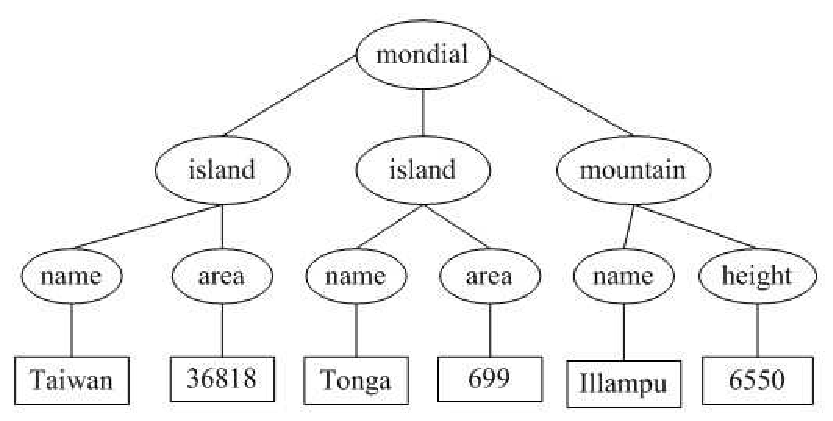
\includegraphics[width=0.4\textwidth]{XML}
	\caption{树状结构}\label{fig:xml}
	\vspace{\baselineskip}
\end{figure}


其插入图片的代码及其说明如下。
\vspace{1em}\noindent\hrule
\begin{verbatim}
	\begin{figure}[htbp]
		\centering
		\includegraphics[width=0.4\textwidth]{文件名(.eps)}
		\caption{标题}\label{标签名(通常为 fig:labelname)}
		\vspace{\baselineskip} %表示图与正文空一行
	\end{figure}
\end{verbatim}

\noindent\hrule

\begin{verbatim}
figure环境的可选参数[htbp]表示浮动图形所放置的位置,h (here)
表示当前位置,t (top)表示页芯顶部,b (bottom)表示页芯底部,
p (page)表示单独一页。在Word等软件中,图片通常插入到当前位置,
如果当前页的剩余空间不够,图片将被移动到下一页,当前页就会出现
很大的空白,其人工调整工作非常不便。由LaTeX提供的浮动图片功能,
总是会按h->t->b->p的次序处理选项中的字母,自动调整图片的位置,
大大减轻了工作量。\centering命令将后续内容转换成每行皆居中的格式。
"\includegraphics"的可选参数用来设置图片插入文中的水平宽度,
一般表示为正文宽度(\textwidth)的倍数。	\caption命令可选
参数“标签名”为英文形式,一般不以图片或表格的数字顺序作为标签,
而应包含一定的图片或表格信息,以便于文中引用(若图片、表格、公
式、章节和参考文献等在文中出现的先后顺序发生了变化,其标注序号
及其文中引用序号也会跟着发生变化,这一点是Word等软件所不能做到
的)。另外,图题或表题并不会因为分页而与图片或表格体分置于两页,
章节等各级标题也不会置于某页的最底部,LaTeX系统会自动调整它们在
正文中的位置,这也是Word等软件所无法匹敌的。\vspace将产生一定
高度的竖直空白,必选参数为负值表示将后续文字位置向上提升,参数
值可自行调整。em为长度单位,相当于大写字母M的宽度。
\vspace{\baselineskip} 表示图与正文空一行。
引用方法:“见图\ref{fig:figname}”、“如图\ref{fig:figname}所示”等。
\end{verbatim}

\noindent\hrule\vspace{1em}

若需要将2张及以上的图片并排插入到一行中,则需要采用\verb|minipage|环境,如图\ref{fig:dd}和图\ref{fig:ds}所示。
\begin{figure}[htbp]
	\centering
	\begin{minipage}{0.4\textwidth}
		\centering
		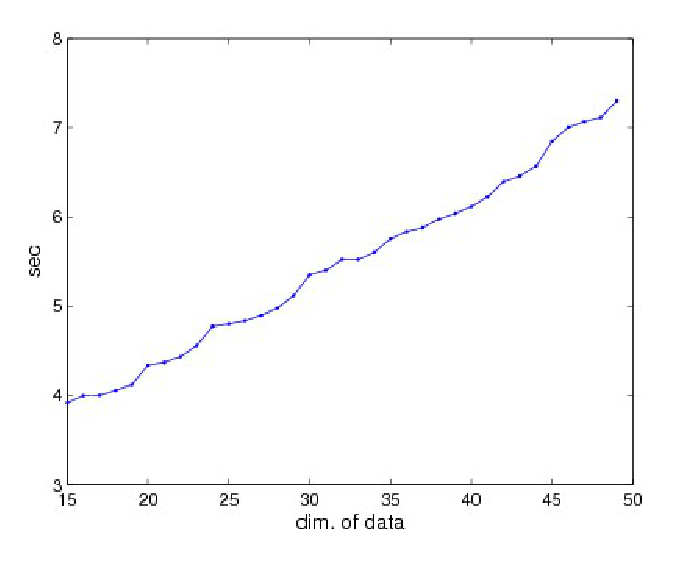
\includegraphics[width=\textwidth]{dataDimensions}
		\caption{数据维数的变化}\label{fig:dd}
	\end{minipage}
	\begin{minipage}{0.4\textwidth}
		\centering
		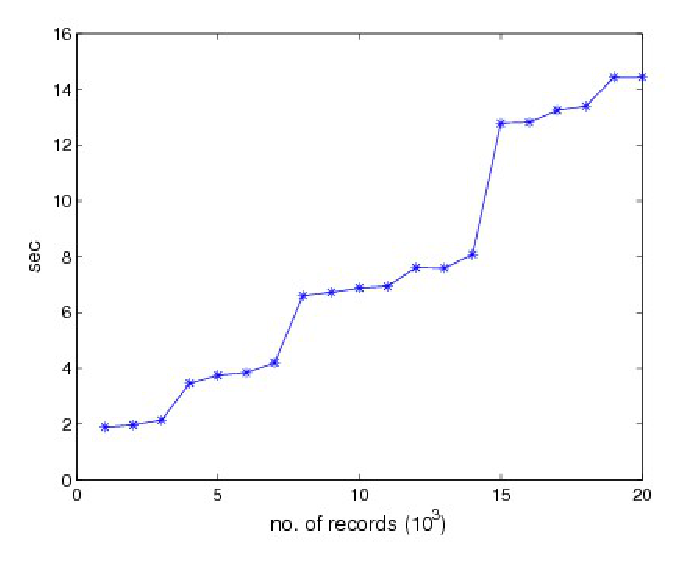
\includegraphics[width=\textwidth]{dataSize}
		\caption{数据规模的变化}\label{fig:ds}
	\end{minipage}
	\vspace{\baselineskip}
\end{figure}

其代码如下所示。

\vspace{1em}\noindent\hrule
\begin{verbatim}
	\begin{figure}[htbp]
		\centering
		\begin{minipage}{0.4\textwidth}
			\centering
			\includegraphics[width=\textwidth]{文件名}
			\caption{标题}\label{fig:f1}
		\end{minipage}
		\begin{minipage}{0.4\textwidth}
			\centering
			\includegraphics[width=\textwidth]{文件名}
			\caption{标题}\label{fig:f2}
		\end{minipage}\vspace{\baselineskip}
	\end{figure}
\end{verbatim}

\noindent\hrule

\begin{verbatim}
minipage环境的必选参数用来设置小页的宽度,若需要在一行中插入
n个等宽图片,则每个小页的宽度应略小于(1/n)\textwidth。
\end{verbatim}

\noindent\hrule

\section{具有子图的图片插入方法}
图中若含有子图时,需要调用subfigure宏包, 如图\ref{fig:subfig}所示。
\begin{figure}[htbp]
	\centering
	\subfigure[Data Dimensions]{\label{fig:subfig:datadim}
		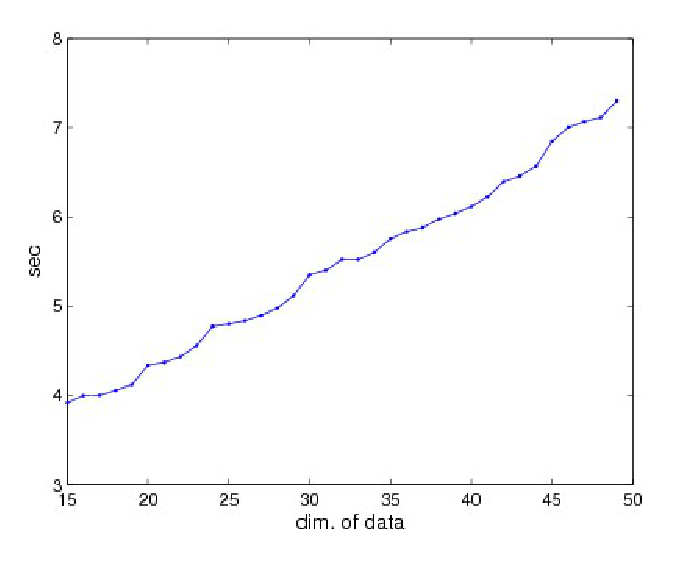
\includegraphics[width=0.4\textwidth]{dataDimensions}}
	\subfigure[Data Size]{\label{fig:subfig:datasize}
		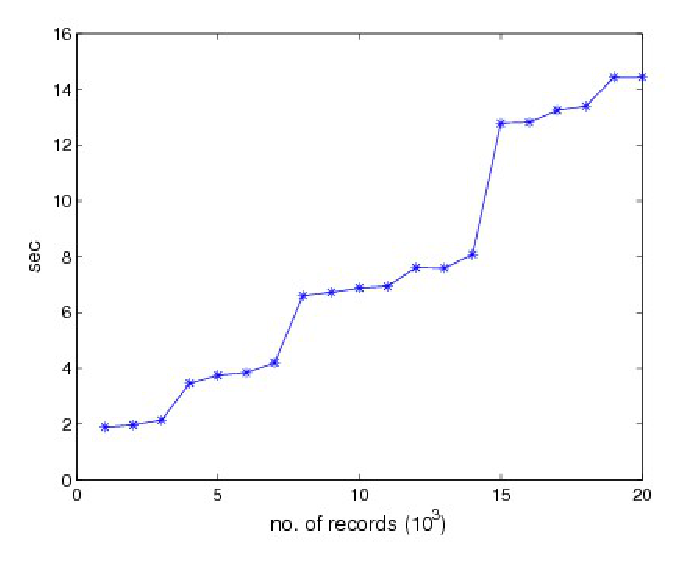
\includegraphics[width=0.4\textwidth]{dataSize}}
	\caption{Scalability of data}\label{fig:subfig}
	\vspace{\baselineskip}
\end{figure}

其代码及其说明如下。
\vspace{1em}\noindent\hrule

\begin{verbatim}
	\begin{figure}[htbp]
		\centering
		\subfigure[第1个子图标题]{
			\label{第1个子图标签(通常为 fig:subfig1:subsubfig1)}
			\includegraphics[width=0.4\textwidth]{文件名}}
		\subfigure[第2个子图标题]{
			\label{第2个子图标签(通常为 fig:subfig1:subsubfig2)}
			\includegraphics[width=0.4\textwidth]{文件名}}
		\caption{总标题}\label{总标签(通常为 fig:subfig1)}
		\vspace{\baselineskip}
	\end{figure}
\end{verbatim}

\noindent\hrule

\begin{verbatim}
	子图的标签实际上可以随意设定,只要不重复就行。但为了更好的
	可读性,我们建议fig:subfig:subsubfig格式命名,这样我们
	从标签名就可以知道这是一个子图引用。引用方法:总图的引用方
	法同本章第1节,子图的引用方法用\ref{fig:subfig:subsubfig}
	来代替。
\end{verbatim}

\noindent\hrule\vspace{1em}

子图的引用示例:如图\ref{fig:subfig:datadim}和图\ref{fig:subfig:datasize}所示。

若想获得插图方法的更多信息,参见网络上的\href{ftp://ftp.tex.ac.uk/tex-archive/info/epslatex.pdf}{Using Imported Graphics in \LaTeX~ and pdf\LaTeX~}文档。
%%% !Mode:: "TeX:UTF-8"
\chapter{表格的绘制方法}
\section{研究生毕业设计论文的绘表规范}
表应有自明性。表格不加左、右边线。表的编排建议采用国际通行的三线表。表内中文书写使用宋体五号字。

每个表格之上均应有表题(由表序和表名组成)。表序一般按章编排,如第1章第一个插表的序号为“表1-1”等。表序与表名之间空两格,
表名使用中文五号字,居中。表名中不允许使用标点符号,表名后不加标点。
表头设计应简单明了,尽量不用斜线。表头中可采用化学,物理量等专业符号。

全表如用同一单位,则将单位符号移至表头右上角,加圆括号。
表中数据应准确无误,书写清楚。数字空缺的格内加横线“-”(占2个数字宽度)。表内文字或数字上、下或左、右相同时,
采用通栏处理方式,不允许用“〃”、“同上”之类的写法。

表内文字使用宋体五号字,垂直居中书写,起行空一格、转行顶格、句末不加标点。
如某个表需要转页接排,在随后的各页上应重复表的编号。编号后加“(续表)”,表题可省略。续表应重复表头。
表格绘制完成之后,与正文空一行。

\section{普通表格的绘制方法}
表格应具有三线表格式,因此需要调用booktabs宏包,其标准格式如表\ref{tab:table1}所示。
\begin{table}[htbp]
	\caption{符合研究生毕业论文绘图规范的表格}\label{tab:table1}
	\vspace{0.5em}\centering\zihao{5}
	\begin{tabular}{ccccc}
		\toprule[1.5pt]
		$D$(in) & $P_u$(lbs) & $u_u$(in) & $\beta$ & $G_f$(psi.in) \\
		\midrule[1pt]
		5       & 269.8      & 0.000674  & 1.79    & 0.04089       \\
		10      & 421.0      & 0.001035  & 3.59    & 0.04089       \\
		20      & 640.2      & 0.001565  & 7.18    & 0.04089       \\
		5       & 269.8      & 0.000674  & 1.79    & 0.04089       \\
		10      & 421.0      & 0.001035  & 3.59    & 0.04089       \\
		20      & 640.2      & 0.001565  & 7.18    & 0.04089       \\
		5       & 269.8      & 0.000674  & 1.79    & 0.04089       \\
		10      & 421.0      & 0.001035  & 3.59    & 0.04089       \\
		20      & 640.2      & 0.001565  & 7.18    & 0.04089       \\
		5       & 269.8      & 0.000674  & 1.79    & 0.04089       \\
		10      & 421.0      & 0.001035  & 3.59    & 0.04089       \\
		20      & 640.2      & 0.001565  & 7.18    & 0.04089       \\
		\bottomrule[1.5pt]
	\end{tabular}
	\vspace{\baselineskip}
\end{table}

其绘制表格的代码及其说明如下。
\vspace{2em}\noindent\hrule

\begin{verbatim}
	\begin{table}[htbp]
		\caption{表标题}\label{标签名(通常为 tab:tablename)}
		\vspace{0.5em}\centering\zihao{5}
		\begin{tabular}{cc...c}
			\toprule[1.5pt]
			表头第1个格   & 表头第2个格   & ... & 表头第n个格  \\
			\midrule[1pt]
			表中数据(1,1) & 表中数据(1,2) & ... & 表中数据(1,n)\\
			表中数据(2,1) & 表中数据(2,2) & ... & 表中数据(2,n)\\
			表中数据(3,1) & 表中数据(3,2) & ... & 表中数据(3,n)\\
			表中数据(4,1) & 表中数据(4,2) & ... & 表中数据(4,n)\\
			...................................................\\
			表中数据(m,1) & 表中数据(m,2) & ... & 表中数据(m,n)\\
			\bottomrule[1.5pt]
		\end{tabular}
		\vspace{\baselineskip}
	\end{table}
\end{verbatim}

\noindent\hrule

\begin{verbatim}
	table环境是一个将表格嵌入文本的浮动环境。\zihao{5}命令将表
	格的字号设置为五号字(10.5pt),在绘制表格结束退出时,不需
	要将字号再改回为\zihao{-4},正文字号默认为小四号字(12pt)。
	tabular环境的必选参数由每列对应一个格式字符所组成:c表示居
	中,l表示左对齐,r表示右对齐,其总个数应与表的列数相同。此
	外,@{文本}可以出现在任意两个上述的列格式之间,其中的文本
	将被插入每一行的同一位置。表格的各行以\\分隔,同一行的各列
	则以&分隔。\toprule、\midrule和\bottomrule三个命令是由booktabs
	宏包提供的,其中\toprule和\bottomrule分别用来绘制表格的第一
	条(表格最顶部)和第三条(表格最底部)水平线,\midrule用来
	绘制第二条(表头之下)水平线,且第一条和第三条水平线的线宽
	为1.5pt,第二条水平线的线宽为1pt。
	引用方法:“如表\ref{tab:tablename}所示”。
\end{verbatim}

\noindent\hrule
\section{长表格的绘制方法}
长表格是当表格在当前页排不下而需要转页接排的情况下所采用的一种表格环境。若长表格仍按照普通表格的绘制方法来获得,
其所使用的\verb|table|浮动环境无法实现表格的换页接排功能,表格下方过长部分会排在表格第1页的页脚以下。为了能够实现长表格的转页接排功能,
需要调用longtable宏包,由于长表格是跨页的文本内容,因此只需要单独的\verb|longtable|环境,所绘制的长表格的格式如表\ref{tab:table2}所示。

此长表格\ref{tab:table2}第2页的标题“编号(续表)”和表头是通过代码自动添加上去的,无需人工添加,若表格在页面中的竖直位置发生了变化,长表格在第2页
及之后各页的标题和表头位置能够始终处于各页的最顶部,也无需人工调整,\LaTeX~系统的这一优点是Word等软件所无法企及的。

下段内容是为了让下面的长表格分居两页,看到表标题“编号(续表)”的效果。摘录于《你若安好,便是晴天 -- 林徽因传》片段:

她叫林徽因,出生于杭州,是许多人梦中期待的白莲。她在雨雾之都伦敦,发生过一场空前绝后的康桥之恋。她爱过三个男子,爱得清醒,也爱得平静。徐志摩为她徜徉在康桥,深情地等待一场旧梦可以归来。梁思成与她携手走过千山万水,为完成使命而相约白头。金岳霖为她终身不娶,痴心不改地守候一世。可她懂得人生飘忽不定,要学会随遇而安。
真正的平静,不是避开车马喧嚣,而是在心中修篱种菊。尽管如流往事,每一天都涛声依旧,只要我们消除执念,便可寂静安然。愿每个人在纷呈世相中不会迷失荒径,可以端坐磐石上,醉倒落花前。
如果可以,请让我预支一段如莲的时光,哪怕将来某一天加倍偿还。这个雨季会在何时停歇,无从知晓。但我知道,你若安好,便是晴天。

\zihao{5}\begin{longtable}{ccc}
	\caption{湖南大学各学院名称一览}\label{tab:table2}
	\vspace{0.5em}                                                                                   \\
	\toprule[1.5pt] 学院名称 & 网址                                                  & 联系电话      \\ \midrule[1pt]
	\endfirsthead
	\multicolumn{3}{c}{表\thetable(续表)}\vspace{0.5em}                                           \\
	\toprule[1.5pt] 学院名称 & 网址                                                  & 联系电话      \\ \midrule[1pt]
	\endhead
	\bottomrule[1.5pt]
	\endfoot
	机械与运载工程学院       & \url{http://mve.hnu.cn/}                              & 88822826      \\
	电气与信息工程学院       & \url{http://eeit.hnu.cn/}                             & 27404775      \\
	电子信息工程学院         & \url{http://www.tju.edu.cn/seie}                      & 27406956      \\
	电气与自动化工程学院     & \url{http://www2.tju.edu.cn/colleges/automate/}       & 27405477      \\
	建筑工程学院             & \url{http://www2.tju.edu.cn/colleges/civil/}          & 27404072      \\
	化工学院                 & \url{http://chemeng.tju.edu.cn/}                      & 27403389      \\
	材料科学与工程学院       & \url{http://mse.tju.edu.cn}                           & 27406693      \\
	建筑学院                 & \url{http://hgw022072.chinaw3.com/}                   & 27402724-2111 \\
	求是学部                                                                                         \\
	管理与经济学部           & \url{ http://sm.tju.edu.cn}                           & 27403423      \\
	理学院                   & \url{ http://www.tju.edu.cn/science/}                 & 27404118      \\
	文法学院                 & \url{ http://www2.tju.edu.cn/colleges/sociology/new/} & 27403691      \\
	信息科学与工程学院       & \url{http://ccc.hnu.cn/}                              & 88821907      \\
	马克思主义学院           & \url{http://www2.tju.edu.cn/colleges/marxism/}        & 27405348      \\
	环境科学与工程学院       & \url{http://www.tju.edu.cn/see}                       & 87402072      \\
	药物科学与技术学院       & \url{http://www2.tju.edu.cn/colleges/pharmtier/}      & 87401830      \\
	教育学院                 & \url{http://soe.tju.edu.cn/}                          & 27401028      \\
	职业技术教育学院         & \url{http://202.113.0.248:8888}                                       \\
	继续教育学院             & \url{http://aectu.tju.edu.cn/}                        & 27406298      \\
	仁爱学院                 & \url{http://www.tjrac.edu.cn/}                        & 68579990      \\
	农业与生物工程学院       & \url{http://202.113.13.169/site/nongxueyuan/}         & 87402171      \\
	国际教育学院             & \url{http://www.ietju.com/}                           & 27406147      \\
	网络教育学院             & \url{http://www.etju.com/}                            & 27426952      \\
\end{longtable}
\zihao{4}
\vspace{\baselineskip}

绘制长表格的代码及其说明如下。
\vspace{1em}\noindent\hrule

\begin{verbatim}
	\zihao{5}\begin{longtable}{cc...c}
		\caption{表标题}\label{标签名(通常为 tab:tablename)}\\
		\toprule[1.5pt] 表头第1个格 & 表头第2个格 & ... & 表头第n个格\\
		 \midrule[1pt]
		\endfirsthead
		\multicolumn{n}{c}{表\thetable(续表)}\vspace{0.5em}\\
		\toprule[1.5pt] 表头第1个格 & 表头第2个格 & ... & 表头第n个格\\
		 \midrule[1pt]
		\endhead
		\bottomrule[1.5pt]
		\endfoot
		表中数据(1,1) & 表中数据(1,2) & ... & 表中数据(1,n)\\
		表中数据(2,1) & 表中数据(2,2) & ... & 表中数据(2,n)\\
		...................................................\\
		表中数据(m,1) & 表中数据(m,2) & ... & 表中数据(m,n)\\
	\end{longtable}\xiaosi
\end{verbatim}

\noindent\hrule
\begin{verbatim}
	在绘制长表格的前面留出一个空白行,并在第2行的一开始全局定
	义长表格的字号为五号字,这样能够保证长表格之前段落的行距
	保持不变。在绘制长表格结束后,需要\zihao{-4}命令重新将字号
	改为小四号字。\endhead之前的文字描述的是第2页及其之后各
	页的标题或表头;\endfirsthead之前的文字描述的是第1页
	的标题和表头,若无此命令,则第1页的表头和标题由\endhead
	命令确定;同理,\endfoot之前的文字描述的是除最后一页之
	外每页的表格底部内容;\endlastfoot之前的文字描述的是最
	后一页的表格底部内容,若无此命令,则最后一页的表格底部内
	容由\endfoot命令确定;由于规范中长表格每页底部内容均相
	同(水平粗线),因此模板中没有用到\endlastfoot命令。
\end{verbatim}

\noindent\hrule
\section{列宽可调表格的绘制方法}
论文中能用到列宽可调表格的情况共有两种:一种是当插入的表格某一单元格内容过长以至于一行放不下的情况,
另一种是当对公式中首次出现的物理量符号进行注释的情况。这两种情况都需要调用tabularx宏包。下面将分别对这两种情况下可调表格的绘制方法进行阐述。
\subsection{表格内某单元格内容过长的情况}
首先给出这种情况下的一个例子如表\ref{tab:table3}所示。
\begin{table}[htbp]
	\caption{最小的三个正整数的英文表示法}\label{tab:table3}
	\vspace{0.5em}\zihao{5}
	\begin{tabularx}{\textwidth}{llX}
		\toprule[1.5pt]
		Value & Name  & Alternate names, and names for sets of the given size                                                                                           \\\midrule[1pt]
		1     & One   & ace, single, singleton, unary, unit, unity                                                                                                      \\
		2     & Two   & binary, brace, couple, couplet, distich, deuce, double, doubleton, duad, duality, duet, duo, dyad, pair, snake eyes, span, twain, twosome, yoke \\
		3     & Three & deuce-ace, leash, set, tercet, ternary, ternion, terzetto, threesome, tierce, trey, triad, trine, trinity, trio, triplet, troika, hat-trick     \\\bottomrule[1.5pt]
	\end{tabularx}
	\vspace{\baselineskip}
\end{table}
绘制这种表格的代码及其说明如下。
\vspace{1em}\noindent\hrule
\begin{verbatim}
	\begin{table}[htbp]
		\caption{表标题}\label{标签名(通常为 tab:tablename)}
		\vspace{0.5em}\zihao{5}
		\begin{tabularx}{\textwidth}{l...X...l}
			\toprule[1.5pt]
			表头第1个格   & ... & 表头第X个格   & ... & 表头第n个格  \\
			\midrule[1pt]
			表中数据(1,1) & ... & 表中数据(1,X) & ... & 表中数据(1,n)\\
			表中数据(2,1) & ... & 表中数据(2,X) & ... & 表中数据(2,n)\\
			.........................................................\\
			表中数据(m,1) & ... & 表中数据(m,X) & ... & 表中数据(m,n)\\
			\bottomrule[1.5pt]
		\end{tabularx}
		\vspace{\baselineskip}
	\end{table}
\end{verbatim}

\noindent\hrule
\begin{verbatim}
	tabularx环境共有两个必选参数:第1个参数用来确定表格的总宽
	度,这里取为排版表格能达到的最大宽度——正文宽度\textwidth;
	第2个参数用来确定每列格式,其中标为X的项表示该列的宽度可调,
	其宽度值由表格总宽度确定。标为X的列一般选为单元格内容过长而
	无法置于一行的列,这样使得该列内容能够根据表格总宽度自动分行。
	若列格式中存在不止一个X项,则这些标为X的列的列宽相同,因此,
	一般不将内容较短的列设为X。标为X的列均为左对齐,因此其余列一
	般选为l(左对齐),这样可使得表格美观,但也可以选为c或r。
\end{verbatim}

\noindent\hrule
\subsection{对物理量符号进行注释的情况}
为使得对公式中物理量符号注释的转行与破折号“———”后第一个字对齐,此处最好采用表格环境。此表格无任何线条,左对齐,
且在破折号处对齐,一共有“式中”二字、物理量符号和注释三列,表格的总宽度可选为文本宽度,因此应该采用\verb|tabularx|环境。
由\verb|tabularx|环境生成的对公式中物理量符号进行注释的公式如式(\ref{eq:1})所示。
%\vspace*{10pt}

\begin{equation}\label{eq:1}
	\ddot{\boldsymbol{\rho}}-\frac{\mu}{R_{t}^{3}}\left(3\mathbf{R_{t}}\frac{\mathbf{R_{t}\rho}}{R_{t}^{2}}-\boldsymbol{\rho}\right)=\mathbf{a}
\end{equation}

\begin{tabularx}{\textwidth}{@{}l@{\quad}r@{———}X@{}}
	式中 & $\bm{\rho}$        & 追踪飞行器与目标飞行器之间的相对位置矢量; \\
	     & $\bm{\ddot{\rho}}$ & 追踪飞行器与目标飞行器之间的相对加速度;   \\
	     & $\mathbf{a}$       & 推力所产生的加速度;                       \\
	     & $\mathbf{R_t}$     & 目标飞行器在惯性坐标系中的位置矢量;       \\
	     & $\omega_{t}$       & 目标飞行器的轨道角速度;                   \\
	     & $\mathbf{g}$       & 重力加速度。
\end{tabularx}
\vspace{\wordsep}

其中生成注释部分的代码及其说明如下。

\vspace{1em}\noindent\hrule

\begin{verbatim}
	\begin{tabularx}{\textwidth}{@{}l@{\quad}r@{— — —}X@{}}
		式中 & symbol-1 & symbol-1的注释内容;\\
		& symbol-2 & symbol-2的注释内容;\\
		.............................;\\
		& symbol-m & symbol-m的注释内容。
	\end{tabularx}\vspace{\wordsep}
\end{verbatim}

\noindent\hrule

\begin{verbatim}
	tabularx环境的第1个参数选为正文宽度,第2个参数里面各个符号
	的意义为:第1个@{}表示在“式中”二字左侧不插入任何文本,
	“式中”二字能够在正文中左对齐,若无此项,则“式中”二字左
	侧会留出一定的空白;@{\quad}表示在“式中”和物理量符号间插
	入一个空铅宽度的空白;@{— — —}实现插入破折号的功能,它
	由三个1/2的中文破折号构成;第2个@{}表示在注释内容靠近正文
	右边界的地方能够实现右对齐。
\end{verbatim}

\noindent\hrule\vspace{1em}

由此方法生成的注释内容应紧邻待注释公式并置于其下方,因此不能将代码放入\verb|table|浮动环境中。但此方法不能实现自动转页接排,
可能会在当前页剩余空间不够时,全部移动到下一页而导致当前页出现很大空白。因此在需要转页处理时,还请您手动将需要转页的代码放入一个
新的\verb|tabularx|环境中,将原来的一个\verb|tabularx|环境拆分为两个\verb|tabularx|环境。

若想获得绘制表格的更多信息,参见网络上的\href{http://www.tug.org/pracjourn/2007-1/mori/}{Tables in \LaTeX~e: Packages and Methods}文档。
%%% !Mode:: "TeX:UTF-8"
\chapter{数学公式的输入方法}
湖南师范大学研究生论文有关公式、数字、年代、符号的书写要求:
\begin{itemize}
	\item 年份一概写全数。例:1998年不能写成98年。
	\item 分数、世纪、年代均以阿拉伯数字表示。例:三分之二写成2/3;二十世纪九十年代写成20世纪90年代。
	\item 公式均需标注公式号,公式号用圆括号,阿拉伯数字表示,按章编排。
	\item 论文中的物理量、量纲及符号等均采用国际标准(SI)和国家标准(GB)。
\end{itemize}
\section{研究生毕业设计论文的公式规范}
论文中的公式应另起行,原则上应居中书写,与周围文字留有足够的空间区分开。
若公式前有文字(如“解”、“假定”等),文字空两格写,公式仍居中写。公式末不加标点。

公式应标注序号,并将序号置于括号内。 公式序号按章编排,如第1章第一个公式序号为“(1-1)”。公式的序号右端对齐。

公式较长时最好在等号“=”处转行,如难实现,则可在$+$、$-$、$\times$、$\div$运算符号处转行,转行时运算符号仅书写于转行式前,不重复书写。

文中引用公式时,一般用“见式(1-1)”或“由公式(1-1)”。

公式中用斜线表示“除”的关系时应采用括号,以免含糊不清,如$a/(b\cos x)$。通常“乘”的关系在前,如$a\cos x/b$而不写成$(a/b)\cos x$。

不能用文字形式表示等式,如:$\textnormal{刚度}=\frac{{\textnormal{受力}}}{{\textnormal{受力方向的位移}}}$。

对于数学公式的输入方法,网络上有一个比较全面权威的文档{\bf{\href{http://tug.ctan.org/cgi-bin/ctanPackageInformation.py?id=voss-mathmode}{Math mode}}}请大家事先大概浏览一下。下面将对学位论文中主要用到的数学公式排版形式进行阐述。

\section{生成\LaTeX~数学公式的两种方法}
对于先前没有接触过\LaTeX~的人来说,编写\LaTeX~数学公式是一件很繁琐的事,尤其是对复杂的数学公式来说,更可以说是一件难以完成的任务。
实际上,生成\LaTeX~数学公式有两种较为简便的方法,一种是基于MathType数学公式编辑器的方法,另一种是基于MATLAB商业数学软件的方法,
下面将分别对这两种数学公式的生成方法作一下简单介绍。

\subsection{基于MathType软件的数学公式生成方法}
MathType是一款功能强大的数学公式编辑器软件,能够用来在文本环境中插入Windows OLE图形格式的复杂数学公式,所以应用比较普遍。但此软件只有30天的试用期,之后若再继续使用则需要付费购买才行。网络上有很多破解版的MathType软件可供下载免费使用,
笔者推荐下载安装版本号在6.5之上的中文破解版。

在安装好MathType之后,若在输入窗口中编写数学公式,复制到剪贴板上的仍然是图形格式的对象。
若希望得到可插入到\LaTeX~编辑器中的文本格式对象,则需要对MathType软件做一下简单的设置:在MathType最上排的按钮中依次选择“参数选项
$\to$转换”,在弹出的对话窗中选中“转换到其它语言(文字):”,在转换下拉框中选择“Tex——LaTeX 2.09 and later”,并将对话框最下方的两个复选框全部勾掉,点击确定,这样,再从输入窗口中复制出来的对象就是文本格式的了,就可以直接将其粘贴到\LaTeX~
编辑器中了。按照这种方法生成的数学公式两端分别有标记\verb|\[|和标记\verb|\]|,在这两个标记之间才是真正的数学公式代码。

若希望从MathType输入窗口中复制出来的对象为图形格式,则只需再选中“公示对象(Windows OLE图形)”即可。

\subsection{基于MATLAB软件的数学公式生成方法}
MATLAB是矩阵实验室(Matrix Laboratory)的简称,是美国MathWorks公司出品的商业数学软件。它是当今科研领域最常用的应用软件之一,
具有强大的矩阵计算、符号运算和数据可视化功能,是一种简单易用、可扩展的系统开发环境和平台。

MATLAB中提供了一个latex函数,它可将符号表达式转化为\LaTeX~数学公式的形式。其语法形式为latex(s),其中,s为符号表达式,
之后再将latex函数的运算结果直接粘贴到\LaTeX~编辑器中。从\LaTeX~数学公式中可以发现,其中可能包含如下符号组合:

\vspace{1em}\noindent\hrule

\begin{verbatim*}
	\qquad=两个空铅(quad)宽度
	\quad=一个空铅宽度
	\;=5/18空铅宽度
	\:=4/18空铅宽度
	\,=3/18空铅宽度
	\!=-3/18空铅宽度
	\ =一个空格
\end{verbatim*}

\noindent\hrule\vspace{1em}

所以最好将上述符号组合从数学公式中删除,从而使数学公式显得匀称美观。

对于Word等软件的使用者来说,在我们通过MATLAB运算得到符号表达式形式的运算结果时,在Word中插入运算结果需要借助于MathType软件,
通过在MathType中输入和MATLAB运算结果相对应的数学表达形式,之后再将MathType数学表达式转换为图形格式粘贴到Word中。实际上,
也可以将MATLAB中采用latex函数运行的结果直接粘贴到MathType中,再继续上述步骤,这样可以大大节省输入公式所需要的时间。
此方法在MathType6.5c上验证通过,若您粘入到MathType中的仍然为从MATLAB中导入的代码,请您更新MathType软件。

\section{数学字体}
在数学模式下,常用的数学字体命令有如下几种:

\vspace{1em}\noindent\hrule
\begin{verbatim}
	\mathnormal或无命令 用数学字体打印文本;
	\mathit             用斜体(\itshape)打印文本;
	\mathbf             用粗体(\bfseries)打印文本;
	\mathrm             用罗马体(\rmfamily)打印文本;
	\mathsf             用无衬线字体(\sffamily)打印文本;
	\mathtt             用打印机字体(\ttfamily)打印文本;
	\mathcal            用书写体打印文本;
\end{verbatim}
\noindent\hrule\vspace{1em}

在学位论文撰写中,只需要用到上面提到的\verb|\mathit|、\verb|\mathbf|和\verb|\mathrm|命令。若要得到Times New Roman的数学字体,则需要调用txfonts宏包(此宏包实际上采用的是Nimbus Roman No9 L字体,
它是开源系统中使用的免费字体,其字符字体与Times New Roman字体几乎完全相同);若要得到粗体数学字体,则需要调用bm宏包。表\ref{tab:fonts}中分别列出了得到阿拉伯数字、拉丁字母和希腊字母
各种数学字体的命令。

\begin{table}[htbp]
	\caption{常用数学字体命令一览}\label{tab:fonts}
	\vspace{0.5em}\centering\zihao{5}
	\begin{tabular}{llll}
		\toprule
		       & 阿拉伯数字\&大写希腊字母 & 大小写拉丁字母          & 小写希腊字母            \\
		\midrule
		斜体   & \verb|\mathit{}|   & \verb|无命令|  & \verb|无命令|  \\
		粗斜体 & \verb|\bm{\mathit{}}|   & \verb|\bm{}| & \verb|\bm{}| \\
		直立体 & \verb|无命令|  & \verb|\mathrm{}| & \verb|字母后加up| \\
		粗体   & \verb|\mathbf{}或\bm{}|  & \verb|\mathbf{}| & \verb|\bm{字母后加up}| \\
		\bottomrule
	\end{tabular}
	\vspace{\baselineskip}
\end{table}

\noindent 下面列出了一些应采用直立数学字体的数学常数和数学符号。

\vspace{-0.5em}
\begin{center}
	\begin{tabularx}{0.9\textwidth}{XX}
		$\mathrm{d}$、 $\mathrm{D}$、 $\mathrm{p}$———微分算子 & $\mathrm{e}$———自然对数之底数 \\
		$\mathrm{i}$、 $\mathrm{j}$———虚数单位                & $\piup$———圆周率               \\
	\end{tabularx}
\end{center}

\section{行内公式}
出现在正文一行之内的公式称为行内公式,例如$f(x)=\int_{a}^{b}\frac{\sin{x}}{x}\mathrm{d}x$。对于非矩阵和非多行形式的行内公式,一般不会使得行距发生变化,而Word等软件却会根据行内公式的竖直距离而自动调节行距,如图\ref{fig:hangju}所示。

\begin{figure}[htbp]
	\centering
	\subfigure[由\LaTeX~系统生成的行内公式]{\label{fig:subfig:latex}
		\fbox{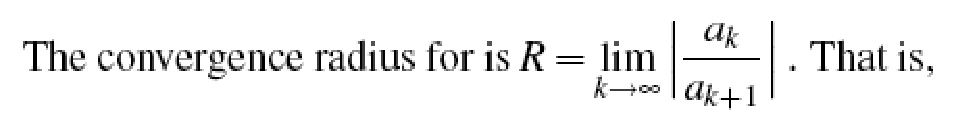
\includegraphics[width=0.55\textwidth]{latex}}}
	\subfigure[由Word软件生成的.doc格式行内公式]{\label{fig:subfig:word}
		\fbox{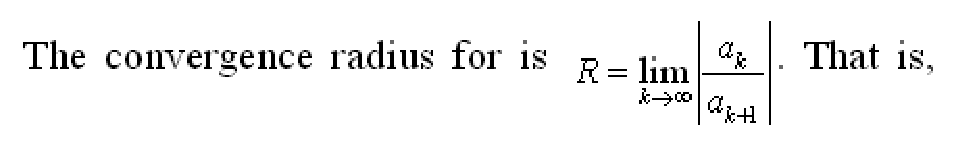
\includegraphics[width=0.55\textwidth]{word}}}
	\subfigure[由Word软件生成的.pdf格式行内公式]{\label{fig:subfig:pdf}
		\fbox{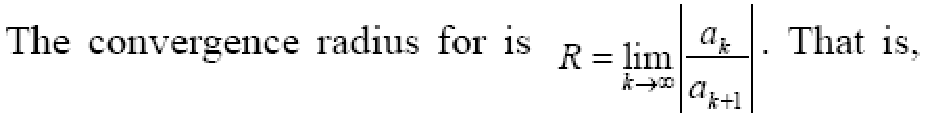
\includegraphics[width=0.55\textwidth]{pdf}}}

	\caption{由\LaTeX~和Word生成的3种行内公式屏显效果}\label{fig:hangju}
	\vspace{-1em}
\end{figure}

这三幅图分别为\LaTeX~和Word生成的行内公式屏显效果,从图中可看出,在\LaTeX~文本含有公式的行内,在正文与公式之间对接工整,行距不变;而在Word文本含有公式的行内,在正文与公式之间对接不齐,行距变大。因此从这一点来说,
\LaTeX~系统在数学公式的排版上具有很大优势。

\LaTeX~提供的行内公式最简单、最有效的方法是采用\TeX~本来的标记———开始和结束标记都写作\$,例如本段开始的例子可由下面的输入得到。
\verb|$f(x)=\int_{a}^{b}\frac{\sin{x}}{x}\mathrm{d}x$|

\section{行间公式}
位于两行之间的公式称为行间公式,每个公式都是一个单独的段落,例如
\[\int_a^b{f\left(x\right)\mathrm{d}x}=\lim_{\left\|\Delta{x_i}\right\|\to 0}\sum_i{f\left(\xi_i\right)\Delta{x_i}}\]
除人工编号外,\LaTeX~各种类型行间公式的标记见表\ref{tab:eqtag}。
\begin{table}[htbp]
	\caption{各种类型行间公式的标记}\label{tab:eqtag}
	\vspace{0.5em}\centering\zihao{5}
	\begin{tabularx}{\textwidth}{cll}
		\toprule
		         & 无编号                     & 自动编号                \\
		\midrule
		单行公式 & \verb|\begin{displaymath}... \end{displaymath}|    & \verb|\begin{equation}... \end{equation}| \\
		         & 或\verb|\[...\]| &                         \\
		多行公式 & \verb|\begin{eqnarray*}... \end{eqnarray*}|    & \verb|\begin{eqnarray}... \end{eqnarray}| \\
		\bottomrule
	\end{tabularx}
\end{table}

另外,在自动编号的某行公式行尾添加标签\verb|\nonumber|,可将该行转换为无编号形式。

行间多行公式需采用\verb|eqnarray|或\verb|eqnarray*|环境,它默认是一个列格式为\verb|rcl|的3列矩阵,并且中间列的字号要小一些,因此通常只将需要对齐的运算符号(通常为等号“=”)置于中间列。

\section{可自动调整大小的定界符}
若在左右两个定界符之前分别添加命令\verb|\left|和\verb|\right|,则定界符可根据所包围公式大小自动调整其尺寸,这可从式(\ref{nodelimiter})和式(\ref{delimiter})中看出。
\begin{equation}\label{nodelimiter}
	(\sum_{k=\frac12}^{N^2})
\end{equation}
\begin{equation}\label{delimiter}
	\left(\sum_{k=\frac12}^{N^2}\right)
\end{equation}
式(\ref{nodelimiter})和式(\ref{delimiter})是在\LaTeX~中分别输入如下代码得到的。
\begin{verbatim}
	(\sum_{k=\frac12}^{N^2})
	\left(\sum_{k=\frac12}^{N^2}\right)
\end{verbatim}
\verb|\left|和\verb|\right|总是成对出现的,若只需在公式一侧有可自动调整大小的定界符,则只要用“.”代替另一侧那个无需打印出来的定界符即可。

若想获得关于此部分内容的更多信息,可参见\href{http://tug.ctan.org/cgi-bin/ctanPackageInformation.py?id=voss-mathmode}{Math mode}文档的第8章“Brackets, braces and parentheses”。

\section{数学重音符号}
数学重音符号通常用来区分同一字母表示的不同变量,输入方法如下(需要调用\verb|amsmath|宏包):

\vspace{0.5em}\noindent\zihao{5}\begin{tabularx}{\textwidth}{Xc|Xc|Xc}
	\verb|\acute| & $\acute{a}$ & \verb|\mathring| & $\mathring{a}$           & \verb|\underbrace| & $\underbrace{a}$          \\
	\verb|\bar| & $\bar{a}$   & \verb|\overbrace| & $\overbrace{a}$          & \verb|\underleftarrow| & $\underleftarrow{a}$      \\
	\verb|\breve| & $\breve{a}$ & \verb|\overleftarrow| & $\overleftarrow{a}$      & \verb|\underleftrightarrow| & $\underleftrightarrow{a}$ \\
	\verb|\check| & $\check{a}$ & \verb|\overleftrightarrow| & $\overleftrightarrow{a}$ & \verb|\underline| & $\underline{a}$           \\
	\verb|\dddot| & $\dddot{a}$ & \verb|\overline| & $\overline{a}$           & \verb|\underrightarrow| & $\underrightarrow{a}$     \\
	\verb|\ddot| & $\ddot{a}$  & \verb|\overrightarrow| & $\overrightarrow{a}$     & \verb|\vec| & $\vec{a}$                 \\
	\verb|\dot| & $\dot{a}$   & \verb|\tilde| & $\tilde{a}$              & \verb|\widehat| & $\widehat{a}$             \\
	\verb|\grave| & $\grave{a}$ & \verb|\underbar| & $\underbar{a}$           & \verb|\widetilde| & $\widetilde{a}$           \\
	\verb|\hat| & $\hat{a}$
\end{tabularx}\vspace{0.5em}
\zihao{4} 当需要在字母$i$和$j$的上方添加重音符号时,为了去掉这两个字母顶上的小点,这两个字母应该分别改用\verb|\imath|和\verb|\jmath|。

如果遇到某些符号不知道该采用什么命令能输出它时,则可通过\href{http://detexify.kirelabs.org/classify.html}{Detexify$^2$网站}来获取符号命令。若用鼠标左键在此网页的方框区域内画出你所要找的符号形状,则会在网页右方列出和你所画符号形状相近的5个符号及其相对应的\LaTeX~输入命令。若所列出的符号中不包括你所要找的符号,还可通过点击“Select from the complete list!”以得分从低到高的顺序列出所有符号及其相对应的\LaTeX~输入命令。

最后,建议大家还以\href{http://tug.ctan.org/cgi-bin/ctanPackageInformation.py?id=voss-mathmode}{Math mode}这篇pdf文档作为主要参考。若要获得最为标准、美观的数学公式排版形式,可以查查文档中是否有和你所要的排版形式相同或相近的代码段,通过修改代码段以获得你所要的数学公式排版形式。


%%% !TEX encoding = UTF-8
\chapter{简要版帮助}
若您已很熟悉\LaTeX~的相关操作,建议阅读这份简要帮助说明。
\section{模板文件结构\label{sec:files}}
整个模板根目录的文件列表如下:
\begin{center}
	\begin{tabular}{|l|p{7.5cm}|l|}
		\hline
		HUNNUthesis.tex          &\TeX{}样例文件             & \textcolor{red}{{*}} \\
		\hline
		HUNNUthesis.cls&包含论文所使用的宏包和全文格式的定义。& \textcolor{red}{{*}} \\
		\hline
		HUNNUThesis.tex& 主文件,包含封面、扉页和其他章节的引用信息。& \textcolor{red}{{*}} \\
		\hline
		preface& 包含毕业设计论文的中英文摘要。& \textcolor{red}{{*}} \\
		\hline
		images& 包含封面用到的湖南师范大学Logo。& \textcolor{red}{{*}} \\
		\hline
		figures& 包含正文中所用到的图片。& \textcolor{red}{{*}} \\
		\hline
		body& 包含正文的所有章节。& \textcolor{red}{{*}} \\
		\hline
		appendix& 附件相关内容& \textcolor{red}{{*}} \\
		\hline
		appendix.tex & 作者的发表论文和参加科研情况说明& \textcolor{red}{{*}} \\
		\hline
		acknowledgements.tex&致谢文件& \textcolor{red}{{*}} \\
		\hline
		statement.tex&原创性说明和版权使用授权说明书。& \textcolor{red}{{*}} \\
		\hline
		hunnubib.bst             & 参考文献样式文件               & \textcolor{red}{{*}} \\
		\hline
		references/reference.bib & bib数据库                  & \textcolor{red}{{*}} \\
		\hline
		official\_documents& 学位论文的撰写格式和开题报告实施管理办法。& \\
		\hline
		clean.bat& 双击此文件,可以用来清理HUNNUThesis.tex在编译之后生成的所有附属文件,如后缀名为.aux,.log,.bak的文件。&  \\
		\hline
	\end{tabular}
\end{center}
注: \textcolor{red}{{*}} 表示\LaTeX{}模板必须的文件。
\subsection{文献引用}
将引文的bib数据库(默认文件名为reference.bib)放入模板根目录下的references文件夹,即可通过插入---文献引用自动产生引文。
\begin{itemize}
	\item 参考文献上标引用
	\begin{itemize}
		\item Journal:An article \upcite{ELIDRISSI94,MELLINGER96}。%参考文献上标
		\item An book \upcite{IEEE-1363,tex,companion}。%参考文献正常引用
		\item Conference:A conference \upcite{kocher99,DPMG,cnproceed}。
		\item Manual:A manual\upcite{NPB2}。
		\item MasterThesis:\upcite{zhubajie,metamori2004,shaheshang,FistSystem01}。
	\end{itemize}
	\item 参考文献正常引用
	\begin{itemize}
	\item Journal:An article \cite{ELIDRISSI94,MELLINGER96}。%参考文献上标
	\item An book \cite{IEEE-1363,tex,companion}。%参考文献正常引用
	\item Conference:A conference \cite{kocher99,DPMG,cnproceed}。
	\item Manual:A manual\cite{NPB2}。
	\item MasterThesis:\cite{zhubajie,metamori2004,shaheshang,FistSystem01}。
\end{itemize}
\end{itemize}
\subsection{伪代码实现}
\begin{algorithm}
	\caption{放进冰箱的大象}\label{算法实例}
	\begin{algorithmic}
		\REQUIRE 有一只大象
		\ENSURE 放进冰箱里
		\FOR {没有剩余的大象}
		\IF {大象比冰箱大}
		\STATE 把大象分割
		\ENDIF
		\ENDFOR
		\STATE 第一步
		\STATE 第二步
		\STATE 第三步
	\end{algorithmic}
	AAA\end{algorithm}
\subsection{代码展示}
可以把你的程序添加到附录里,展示自己的工作。
\begin{lstlisting}[language={[ANSI]C},
numbers=left,
numberstyle=\tiny,
basicstyle=\small\ttfamily,
stringstyle=\color{purple},
keywordstyle=\color{blue}\bfseries,
commentstyle=\color{olive},
directivestyle=\color{blue},
showstringspaces=false]
	#include <stdio.h>
	int main(int argc, char ** argv)
	{
		/*打印Hello,world*/
		printf("Hello, world!\n");
		
		return 0;
	}
\end{lstlisting}
\section{依赖}
HUNNUthesis依赖于以下宏包,这些宏包在常见的\LaTeX{}发行版中都包括,在安装使用之前,请确定你的\TeX{}发行版中都已正常安装这些宏包
\begin{table}[H]
	\centering
	\begin{tabular}{cccc}
\hline
{natbib} & {amsmath} & {amsfonts} & {amssymb} \\

{graphicx} & {subfigure} & {mathptmx} & {float} \\

{fontenc} & {booktabs} & {setspace} & {listings} \\

{xcolor} & {multirow} & {fancyhdr} & {etoolbox} \\

{tocloft} & {array} & {makecell} & {forloop} \\

{xstring} & {hyperref} & {cleveref} & {enumitem} \\

{algorithm} & {algorithmic} & {caption} & {ifthen} \\

{titlesec} & {ulem} & {amssymb} & {wasysym} \\

{flafter} & {booktabs} & {longtable} & {tabularx} \\

{setspace} & {subfigure} & {enumitem} & {calc } \\

{txfonts} & {bm} & {ntheorem} & {fancyvrb} \\

{xcolor} & {--} & {--} & {--} \\
\hline
	\end{tabular}
\end{table}
如果你尚未安装这些宏包,可以启动你的 \TeX{} 发行版的宏包管理器
来安装;或者到 \url{http://www.ctan.org} 上搜索下载并安装。
\section{基本设置}
\begin{enumerate}
	\item 论文正文所用图片搜索路径默认设置为模板根目录下的figures/。
	\item bib数据库默认设置为模板根目录下的references/reference.bib。 其中bib文件可由任意文献库管理软件自动生成
\end{enumerate}
\section{文字命令}
\subsection{常用命令}
\LaTeX 提供了一系列命令,用于修改字体、字号、数字等的呈现形式。
\subsubsection{字体}
ctex宏包及其文档类可直接使用以下六种字体:
\vspace{1em}\noindent\hrule
\begin{verbatim}
宋体: \songti       启用宋体  {\songti 宋体}。
黑体: \heiti        启用黑体  {\heiti 黑体}。
仿宋: \fangsong    启用仿宋   {\fangsong 仿宋}。
楷书: \kaishu       启用楷书   {\kaishu 楷书}。
隶书: \lishu        启用隶书  {\lishu 隶书}。
幼圆: \youyuan     启用幼圆   {\youyuan 幼圆}。
\end{verbatim}
\noindent\hrule\vspace{1em}

宋体:{\songti 宋体};黑体:{\heiti 黑体};仿宋:{\fangsong 仿宋};楷书:{\kaishu 楷书};隶书: {\lishu 隶书};幼圆: {\youyuan 幼圆}。
\subsubsection{字号}
{\bf 字号}%

\begin{center}
	\begin{tabular}{cccccccc}
		\toprule
		初号 & 小初 & 一号 & 小一 & 二号 & 小二 & 三号 & 小三 \\
		0    & -0   & 1    & -1   & 2    & -2   & 3    & -3   \\
		\hline
		四号 & 小四 & 五号 & 小五 & 六号 & 小六 & 七号 & 八号 \\
		4    & -4   & 5    & -5   & 6    & -6   & 7    & 8    \\
		\bottomrule
	\end{tabular}
\end{center}

\vspace{1em}\noindent\hrule
\begin{verbatim}
{\zihao{0}初号}; \dots {\zihao{4}四号};\dots 
\zihao{7}{七号} \zihao{4}
\end{verbatim}
\noindent\hrule\vspace{1em}

{\zihao{0}初号}; \dots {\zihao{4}四号};\dots \zihao{7}{七号}
\zihao{4}
%%% !TEX encoding = UTF-8
\addcontentsline{toc}{chapter}{结论}
\chapter*{结\quad 论}
结论单独作为一章排写,但不加章号。结论是毕业论文(设计)的总结,是整篇论文(设计)的归宿。要求精炼、准确地概述全文的主要观点:或自己赞成的观点、或自己反对的观点、或自己的创造性工作与新的见解及其意义和作用,还进一步提出需要讨论的问题和建议等。特别提醒这部分不是写你做毕业设计(论文)的感想,不是抒情。下面是一个分页符,可以另起一页

结论应是作者在学位论文研究过程中所取得的创新性成果的概要总结,不能与摘要混为一谈。
学位论文结论应包括论文的主要结果、创新点、展望三部分,在结论中应概括论文的核心观点,
明确、客观地指出本研究内容的创新性成果(含新见解、新观点、方法创新、技术创新、理论创新),并指出今后进一步在本研究方向进行研究工作的展望与设想。
对所取得的创新性成果应注意从定性和定量两方面给出科学、准确的评价,分(1)、(2)、(3)…条列出,宜用“提出了”、“建立了”等词叙述。

结论应是作者在学位论文研究过程中所取得的创新性成果的概要总结,不能与摘要混为一谈。
学位论文结论应包括论文的主要结果、创新点、展望三部分,在结论中应概括论文的核心观点,
明确、客观地指出本研究内容的创新性成果(含新见解、新观点、方法创新、技术创新、理论创新),并指出今后进一步在本研究方向进行研究工作的展望与设想。
对所取得的创新性成果应注意从定性和定量两方面给出科学、准确的评价,分(1)、(2)、(3)…条列出,宜用“提出了”、“建立了”等词叙述。

结论应是作者在学位论文研究过程中所取得的创新性成果的概要总结,不能与摘要混为一谈。
学位论文结论应包括论文的主要结果、创新点、展望三部分,在结论中应概括论文的核心观点,
明确、客观地指出本研究内容的创新性成果(含新见解、新观点、方法创新、技术创新、理论创新),并指出今后进一步在本研究方向进行研究工作的展望与设想。
对所取得的创新性成果应注意从定性和定量两方面给出科学、准确的评价,分(1)、(2)、(3)…条列出,宜用“提出了”、“建立了”等词叙述。

结论应是作者在学位论文研究过程中所取得的创新性成果的概要总结,不能与摘要混为一谈。
学位论文结论应包括论文的主要结果、创新点、展望三部分,在结论中应概括论文的核心观点,
明确、客观地指出本研究内容的创新性成果(含新见解、新观点、方法创新、技术创新、理论创新),并指出今后进一步在本研究方向进行研究工作的展望与设想。
对所取得的创新性成果应注意从定性和定量两方面给出科学、准确的评价,分(1)、(2)、(3)…条列出,宜用“提出了”、“建立了”等词叙述。
\end{verbatim}

\noindent\hrule\vspace{1em}

那么,编译的时候就只编译未加\%的一章,在这个例子中,即本章chapter1。

理论上,并不一定要把每章放在不同的文件中。但是这种自顶向下,分章节写作、编译的方法有利于提高效率,大大减少Debug过程中的编译时间,同时减小风险。
\section{参考文献生成方法}
\LaTeX~具有插入参考文献的能力。Google Scholar网站上存在兼容BibTeX的参考文献信息,通过以下几个步骤,可以轻松完成参考文献的生成。
\begin{itemize}
	\item 在\href{http://scholar.google.com/}{谷歌学术搜索}中,
	      点击\href{http://scholar.google.com/scholar_preferences?hl=en&as_sdt=0,5}{学术搜索设置}。
	\item 页面打开之后,在{\bf 文献管理软件}选项中选择{\bf 显示导入BibTeX的链接},单击保存设置,退出。
	\item 在谷歌学术搜索中检索到文献后,在文献条目区域单击导入BibTeX选项,页面中出现文献的引用信息。
	\item 将文献引用信息的内容复制之后,添加到references文件夹下的reference.bib中。
\end{itemize}
\section{编译注意事项}
\begin{enumerate}
	\item 由于模板使用UTF-8编码,所以源文件应该保存成UTF-8格式,否则可能出现中文字符无法识别的错误。
	      本模板中每一个.tex文件的文件的开头已经加上一行:\\
	      \verb|% !Mode:: "TeX:UTF-8"|\\
	      这样可以确保.tex文件默认使用UTF-8的格式打开。读者如果删去此行,很有可能会导致中文字符显示乱码。
	\item 建议采用以下编译方式:

	{\color{red}\heiti\bfseries XeLaTeX --> BibTeX --> XeLaTeX --> XeLaTeX}
\end{enumerate}
\section{系统要求}
TeX Live 2019或以上版本。使用推荐的TexStudio编辑器,可以完成文件的编辑和编译工作。
\section{\TeX~简介}
以下内容是milksea@bbs.ctex.org撰写的关于\TeX~的简单介绍,略有改动。
注意这不是一个入门教程,不讲\TeX~系统的配置安装,也不讲具体的\LaTeX~代码。
这里仅仅试图以一些只言片语来解释:
进入这个门槛之前新手应该知道的注意事项,以及遇到问题以后该去如何解决问题。
\subsection{什么是 \TeX/\LaTeX~,我是否应该选择它?}
\TeX~是最早由高德纳(Donald Knuth)教授创建的一门标记式宏语言,
用来排版科技文章,尤其擅长处理复杂的数学公式。\TeX~同时也是处理这一语言的排版软件。
\LaTeX~是 Leslie Lamport 在\TeX~基础上按内容/格式分离和模块化等思想建立的一集\TeX~上的格式。

\TeX~本身的领域是专业排版领域
但现在TeX/LaTeX也被广泛用于生成电子文档甚至幻灯片等,\TeX~语言的数学部分
偶尔也在其他一些地方使用。但注意\TeX~并不适用于文书处理(Microsoft Office 的领域,以前和现在都不是)。

选择使用\TeX/\LaTeX~的理由包括:
\begin{itemize}
	\item 免费软件;
	\item 专业的排版效果;
	\item 是事实上的专业数学排版标准;
	\item 广泛的西文期刊接收甚或只接收 LaTeX 格式的投稿;
	\item[] ……
\end{itemize}
不选择使用\TeX/\LaTeX~的理由包括:
\begin{itemize}
	\item 需要相当精力学习;
	\item 图文混合排版能力不够强;
	\item 仅在数学、物理、计算机等领域流行;
	\item 中文期刊的支持较差;
	\item[] ……
\end{itemize}

请尽量清醒看待网上经常见到的关于\TeX~与其他软件的优劣比较和口水战。在选择使用或离开之前,请先考虑
\TeX~的应用领域,想想它是否适合你的需要。
\subsection{我该用什么编辑器?}
编辑器功能有简有繁,特色不一,从简单的纯文本编辑器到繁复的 Emacs,因人而易。基本功能有语法高亮、方便编译预览就很好了,扩充功能和定制有无限的可能。初学者可以使用功能简单、使用方便的专用编辑器,如TexStudio、TeXWorks、Kile、WinEdt等,或者类似所见即所得功能的LyX;熟悉的人可以使用定制性更强的Notepad++、SciTE、Vim、Emacs 等。这方面的介绍很多,一开始不妨多试几种,找到最适合自己的才是最好的。

另外提醒一句,编辑器只是工作的助手,不必把它看得太重。
\subsection{我应该看什么\LaTeX~读物?}
这不是一个容易回答的问题,因为有许多选择,也同样有许多不合适的选择。
这里只是选出一个比较好的答案。更多更详细的介绍可以在版面和网上寻找(注意时效)。

近两年\TeX~的中文处理发展很快,目前没有哪本书在中文处理方面给出一个最新进展的合适综述,
因而下面的介绍也不主要考虑中文处理。

\begin{enumerate}
	\item 我能阅读英文。
	      \begin{enumerate}
		      \item 迅速入门:ltxprimer.pdf (LaTeX Tutorials: A Primer, India TUG)
		      \item 系统学习:A Guide to LaTeX, 4th Edition, Addison-Wesley
		            有机械工业出版社的影印版(《\LaTeX{}实用教程》)
		      \item 深入学习:要读许多书和文档,TeXbook 是必读的
		      \item 细节学习:去读你使用的每一个宏包的说明文档
		      \item 专题学习:阅读讲数学公式、图形、表格、字体等的专题文档
	      \end{enumerate}
	\item 我更愿意阅读中文。
	      \begin{enumerate}
		      \item 迅速入门:lnotes.pdf (LaTeX Notes, 1.20, Alpha Huang)
		      \item 系统学习:《\LaTeXe{}科技排版指南》,邓建松(电子版)
		            如果不好找,可以阅读《\LaTeXe~入门与提高》第二版,陈志杰等,或者 《\LaTeXe~完全学习手册》,胡伟
		      \item 深入学习:TeXbook0.pdf(特可爱原本,TeXbook 的中译,xianxian)
		      \item 具体问题释疑:CTeX-FAQ.pdf,\\
		            吴凌云,\url{http://www.ctex.org/CTeXFAQ}
	      \end{enumerate}
\end{enumerate}

遇见问题和解决问题的过程可以快速提高自己的技能,建议此时:
\begin{itemize}
	\item 利用Google搜索。
	\item 清楚,扼要地提出你的问题。
\end{itemize}

\subsection{什么知识会过时?什么不会?}
\TeX~是排版语言,也是广泛使用的软件,并且不断在发展中;
因此,总有一些东西会很快过时。作为学习\TeX~的人,
免不了要看各种各样的书籍、电子文档和网络论坛上的只言片语,
因此了解什么知识会迅速过时,什么知识不会是十分重要的。

最稳定的是关于Primitive \TeX~和Plain \TeX~的知识,也就是 Knuth
在他的《The TeXbook》中介绍的内容。因为\TeX~系统开发的初衷就是稳定性,要求今天的文档到很久以后仍可以得到完全相同的结果,
因此 Knuth 限定了他的\TeX~语言和相关实现的命令、语法。这些内容许多年来就没有多少变化,
在未来的一些年里也不会有什么变化。
Primitive \TeX~和 Plain \TeX~的知识主要包括 \TeX~排版的基本算法和原理,
盒子的原理,底层的 \TeX~命令等。其中技巧性的东西大多在宏包设计中,
初学者一般不会接触到很多;而基本原理则是常常被提到的,
譬如,\TeX~把一切排版内容作为盒子(box)处理。

相对稳定的是关于基本\LaTeXe~的知识,也包括围绕\LaTeXe~的一些核心宏包的知识。\LaTeXe~是自1993年以来的一个稳定的\LaTeX~版本,直到最近的一次修订(2005 年)都没有大的变动。\LaTeX~的下一个计划中的版本\LaTeX 3遥遥无期,在可预见的将来,\LaTeXe~不会过时。\LaTeXe~的知识是目前大部分\LaTeX~书籍的主体内容。关于\LaTeX~的标准文档类(article、report、book、letter、slide等),关于基本数学公式的输入,文档的章节层次,表格和矩阵,图表浮动体,LR 盒子与段落盒子……这些\LaTeX~的核心内容都是最常用的,相对稳定的。与\LaTeXe~相匹配的核心宏包,如graphics(x)、ifthen、fontenc、doc等,也同样是相对稳定的。还有一些被非常广泛应用的宏包,如amsmath系列,也可以看作是相对稳定的。

简单地说,关于基本\TeX/\LaTeX~的语言,都是比较稳定的。与之对应,实现或者支持\TeX/\LaTeX~语言的软件,包括在\TeX/\LaTeX~基础上建立的新的宏,都不大稳定。

容易过时的是关于第三方\LaTeX~宏包的知识、第三方\TeX~工具的知识,以及新兴\TeX~相关软件的知识等。\TeX~和\LaTeX~语言是追求稳定的;但无论是宏包还是工具,作为不断更新软件,它们是不稳定的。容易过时的技术很多,而且现在广泛地出现在几乎所有\LaTeX~文档之中,因此需要特别引起注意:宏包的过时的原因可能是宏包本身的升级换代带来了新功能或不兼容,也可能是同一功能的更新更好的宏包代替了旧的宏包。前者的典型例子比如绘图宏包PGF/TikZ,现在的2.00版功能十分强大,和旧的1.1x版相差很大,和更旧的0.x版本则几乎完全不同;后者的典型例子比如caption宏包先是被更新的caption2宏包代替,后来caption宏包更新又使得caption2 宏包完全过时。——安装更新的发行版可以避免使用过旧的宏包;认真阅读宏包自带的文档而不是搜索得到的陈旧片断可以避免采用过时的代码。

工具过时的主要原因也是升级换代和被其他工具替换。前者的典型例子是编辑器WinEdt在5.5以后的版本支持UTF-8编码,而旧版本不支持;后者的典型例子是中文字体安装工具从GBKFonts到xGBKFonts到FontsGen不断被取代。图形插入是一个在\TeX~实现、宏包与外围工具方面都更新很快的东西。在过去,最常用的输出格式是PS(PostScript)格式,因此插入的图像以EPS为主流。使用Dvips为主要输出工具,外围工具有GhostScript、bmeps等等,相关宏包有graphics等,相关文档如《\LaTeXe{} 插图指南》。

但凡提及“\LaTeX~只支持EPS图形”的,就是这个过时的时代的产物。事实上\TeX/\LaTeX~并不限定任何图形格式,只不过是当时的输出格式(PS)和工具(Dvips)对EPS情有独钟而已。后来 PDF 格式成为主流。pdf\TeX~、DVIPDFM、DVIPDFMx、XeTeX工具则主要支持PDF、PNG、JPG格式的图形,涉及一系列工具如ImageMagick、ebb等。

值得特别提出注意的就是,中文处理也一起是更新迅速、容易过时的部分。而且因为中文处理一直没有一个“官方”的“标准”做法,软件、工具、文档以及网上纷繁的笔记也就显得相当混乱。从八十年代开始的CCT系统、天元系统,到后来的CJK方式,到近来的XeTeX和LuaTeX 方式,中文处理的原理、软件、宏包、配置方式等都在不断变化中。
\section{免责声明}
本模板依据《湖南师范大学研究生学位论文的撰写格式》编写,适用于所有博士、硕士生的学位论文编写。然而,作者不保证本模板完全符合学校要求,也不对由此带来的风险和损失承担任何责任。
%%% !Mode:: "TeX:UTF-8"
\chapter{图片的插入方法}
\section{研究生毕业论文的插图规范}
图应有自明性。插图应与文字紧密配合,文图相符,内容正确。选图要力求精练,插图、照片应完整清晰。图中文字和数字等字号用宋体五号字。

机械工程图:采用第一角投影法,严格按照GB4457---GB131-83《机械制图》标准规定。

数据流程图、程序流程图、系统流程图等按GB1526-89标准规定。

电气图:图形符号、文字符号等应符合有关标准的规定。

流程图:必须采用结构化程序并正确运用流程框图。

对无规定符号的图形应采用该行业的常用画法。

坐标图的坐标线均用细实线,粗细不得超过图中曲线,有数字标注的坐标图,必须注明坐标单位。

照片图要求主题和主要显示部分的轮廓鲜明,便于制版。如用放大或缩小的复制品,必须清晰,反差适中。照片上应有表示目的物尺寸的标度。

引用文献图表必须标注出处。

\subsection{图题及图中说明}
每个图均应有图题(由图序和图名组成),图名在图序之后空两格排写。图序按章编排,如第1章第一个插图的图号为“图1-1”等。
图题置于图下,要求中文用宋体五号字,位置居中。有图注或其它说明时应置于图题之上。引用图应注明出处,在图题右上角加引用文献号。
图中若有分图时,分图题置于分图之下或图题之下,分图号用a)、b)等表示。

图中各部分说明应采用中文(引用的外文图除外)或数字项号,各项文字说明置于图题之上(有分图题者,置于分图题之上)。

\subsection{插图编排}
插图之前,文中必须有关于本插图的提示,如“见图1-1”、“如图1-1所示”等。插图与其图题为一个整体,不得拆开排写于两页。
插图处的该页空白不够排写该图整体时,则可将其后文字部分提前排写,将图移到次页。

\section{\LaTeX~中推荐使用的图片格式}
在\LaTeX~中应用最多的图片格式是EPS(Encapsulated PostScript)格式,它是一种专用的打印机描述语言,常用于印刷或打印输出。
EPS格式图片可通过多种方式生成,这里介绍一款功能强大的免费图片处理软件———\href{http://www.imagemagick.org/}{ImageMagick},
此软件可将其它格式图片转换为EPS格式图片,同时还可以锐化图片,使图片的局部清晰一些。

此软件对图片的格式转换操作都是在命令提示符(cmd.exe)中实现的,可以通过“开始$\to$运行$\to$输入cmd$\to$回车”或
“开始$\to$程序$\to$附件$\to$命令提示符”找到它。在命令提示符下,首先采用“盘符命令”或“cd命令”将当前目录改为待处理图片所在的目录,
在此目录下就可通过convert命令将图片转换为EPS格式,其命令的语法格式为

\indent\verb|convert [可选参数] 原文件名.原扩展名 新文件名.eps|.

若convert命令中无可选参数,则将原来的图片格式直接转换为EPS格式,对图片不进行任何处理,这也是最常用的方法。
也可以选用可选参数,可选参数有很多选择,但最常用的有如下两个:

\verb|-sharpen radius{xsigma}|———此参数用来锐化图片,一般用在图片像素不高,需要提高图片清晰度的情况下。其中radius只能为整数,
它用来确定转换命令采取哪一种锐化算法,我们可以只取radius为0;sigma为所采取算法的锐化度,它的取值为$0.1 - 3$之间的任意一个浮点数,
数值越大,锐化程度也越大,通常取为$0.1 - 3$之间;x在参数中为分隔符。
\verb|-resize geometry|———此参数用来改变图片的大小,若图片的存储空间过大,可通过此命令缩小图片尺寸,但同时也将导致图片像素降低,
其具体用法请参见\href{http://www.imagemagick.org/script/command-line-options.php#resize}{-resize geometry的官方说明}。

除此之外,一些文字处理软件和科学计算软件也支持生成EPS格式的文件,请使用“另存为”功能查看某款软件是否能够将图片以EPS格式的形式保存。

\section{单张图片的插入方法}
单张图片独自占一行的插入形式如图\ref{fig:xml}所示。
\begin{figure}[htbp]
	\centering
	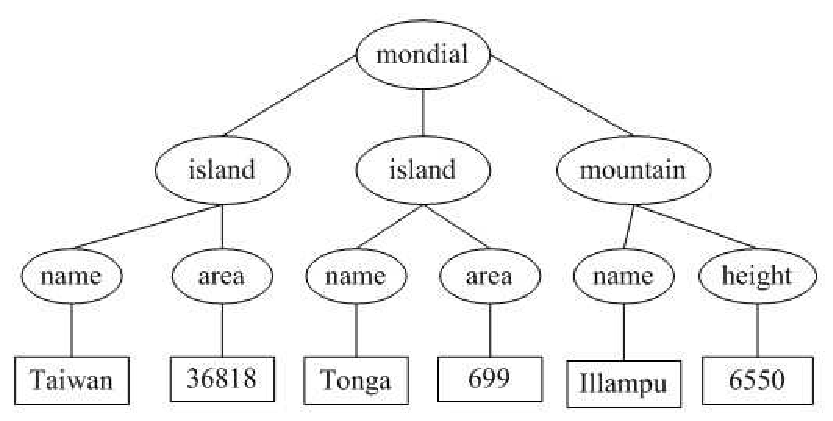
\includegraphics[width=0.4\textwidth]{XML}
	\caption{树状结构}\label{fig:xml}
	\vspace{\baselineskip}
\end{figure}


其插入图片的代码及其说明如下。
\vspace{1em}\noindent\hrule
\begin{verbatim}
	\begin{figure}[htbp]
		\centering
		\includegraphics[width=0.4\textwidth]{文件名(.eps)}
		\caption{标题}\label{标签名(通常为 fig:labelname)}
		\vspace{\baselineskip} %表示图与正文空一行
	\end{figure}
\end{verbatim}

\noindent\hrule

\begin{verbatim}
figure环境的可选参数[htbp]表示浮动图形所放置的位置,h (here)
表示当前位置,t (top)表示页芯顶部,b (bottom)表示页芯底部,
p (page)表示单独一页。在Word等软件中,图片通常插入到当前位置,
如果当前页的剩余空间不够,图片将被移动到下一页,当前页就会出现
很大的空白,其人工调整工作非常不便。由LaTeX提供的浮动图片功能,
总是会按h->t->b->p的次序处理选项中的字母,自动调整图片的位置,
大大减轻了工作量。\centering命令将后续内容转换成每行皆居中的格式。
"\includegraphics"的可选参数用来设置图片插入文中的水平宽度,
一般表示为正文宽度(\textwidth)的倍数。	\caption命令可选
参数“标签名”为英文形式,一般不以图片或表格的数字顺序作为标签,
而应包含一定的图片或表格信息,以便于文中引用(若图片、表格、公
式、章节和参考文献等在文中出现的先后顺序发生了变化,其标注序号
及其文中引用序号也会跟着发生变化,这一点是Word等软件所不能做到
的)。另外,图题或表题并不会因为分页而与图片或表格体分置于两页,
章节等各级标题也不会置于某页的最底部,LaTeX系统会自动调整它们在
正文中的位置,这也是Word等软件所无法匹敌的。\vspace将产生一定
高度的竖直空白,必选参数为负值表示将后续文字位置向上提升,参数
值可自行调整。em为长度单位,相当于大写字母M的宽度。
\vspace{\baselineskip} 表示图与正文空一行。
引用方法:“见图\ref{fig:figname}”、“如图\ref{fig:figname}所示”等。
\end{verbatim}

\noindent\hrule\vspace{1em}

若需要将2张及以上的图片并排插入到一行中,则需要采用\verb|minipage|环境,如图\ref{fig:dd}和图\ref{fig:ds}所示。
\begin{figure}[htbp]
	\centering
	\begin{minipage}{0.4\textwidth}
		\centering
		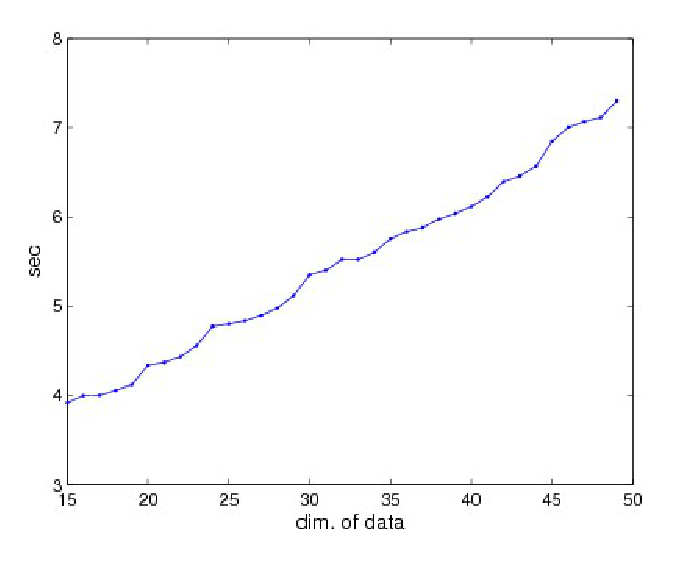
\includegraphics[width=\textwidth]{dataDimensions}
		\caption{数据维数的变化}\label{fig:dd}
	\end{minipage}
	\begin{minipage}{0.4\textwidth}
		\centering
		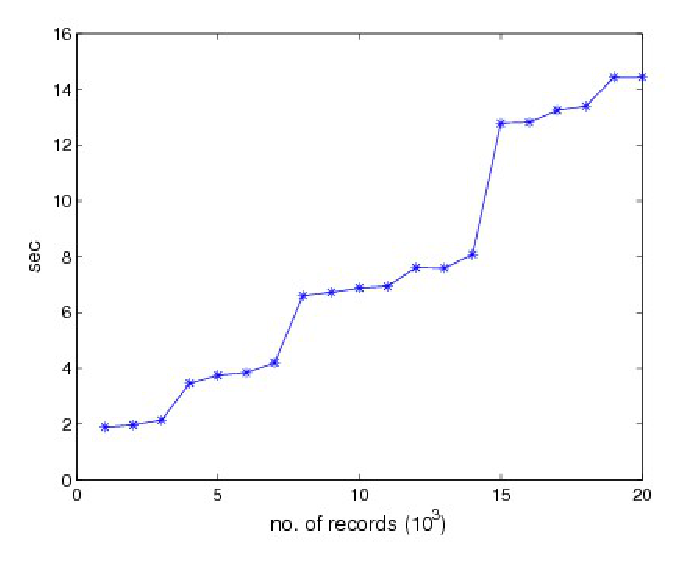
\includegraphics[width=\textwidth]{dataSize}
		\caption{数据规模的变化}\label{fig:ds}
	\end{minipage}
	\vspace{\baselineskip}
\end{figure}

其代码如下所示。

\vspace{1em}\noindent\hrule
\begin{verbatim}
	\begin{figure}[htbp]
		\centering
		\begin{minipage}{0.4\textwidth}
			\centering
			\includegraphics[width=\textwidth]{文件名}
			\caption{标题}\label{fig:f1}
		\end{minipage}
		\begin{minipage}{0.4\textwidth}
			\centering
			\includegraphics[width=\textwidth]{文件名}
			\caption{标题}\label{fig:f2}
		\end{minipage}\vspace{\baselineskip}
	\end{figure}
\end{verbatim}

\noindent\hrule

\begin{verbatim}
minipage环境的必选参数用来设置小页的宽度,若需要在一行中插入
n个等宽图片,则每个小页的宽度应略小于(1/n)\textwidth。
\end{verbatim}

\noindent\hrule

\section{具有子图的图片插入方法}
图中若含有子图时,需要调用subfigure宏包, 如图\ref{fig:subfig}所示。
\begin{figure}[htbp]
	\centering
	\subfigure[Data Dimensions]{\label{fig:subfig:datadim}
		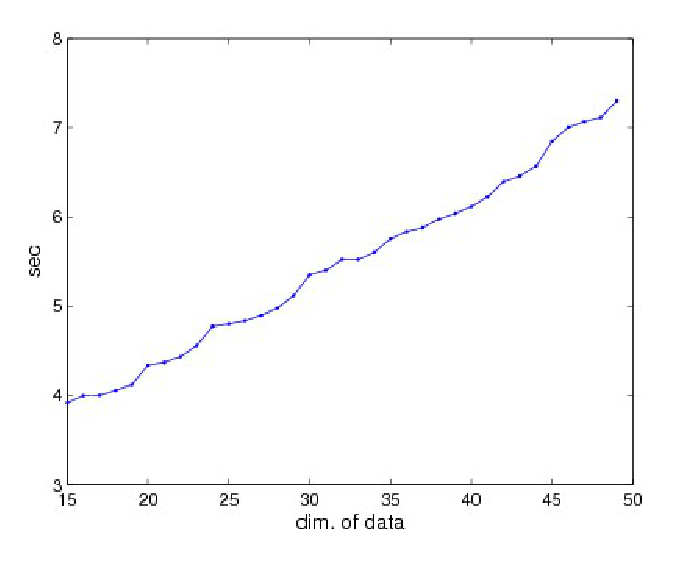
\includegraphics[width=0.4\textwidth]{dataDimensions}}
	\subfigure[Data Size]{\label{fig:subfig:datasize}
		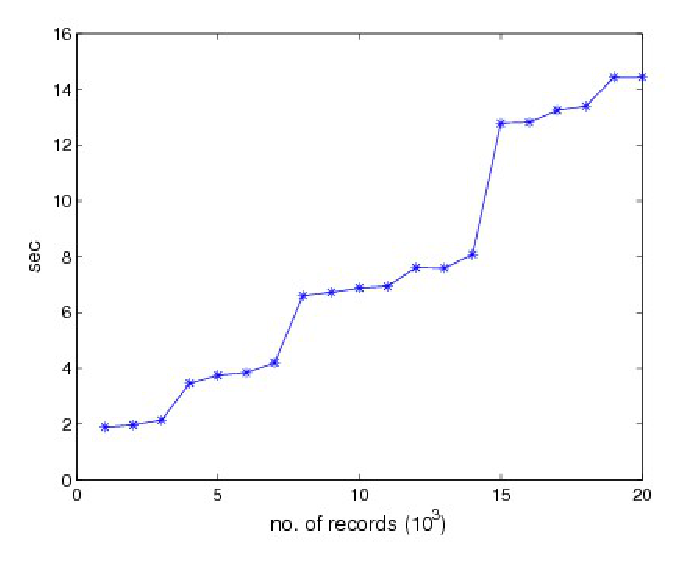
\includegraphics[width=0.4\textwidth]{dataSize}}
	\caption{Scalability of data}\label{fig:subfig}
	\vspace{\baselineskip}
\end{figure}

其代码及其说明如下。
\vspace{1em}\noindent\hrule

\begin{verbatim}
	\begin{figure}[htbp]
		\centering
		\subfigure[第1个子图标题]{
			\label{第1个子图标签(通常为 fig:subfig1:subsubfig1)}
			\includegraphics[width=0.4\textwidth]{文件名}}
		\subfigure[第2个子图标题]{
			\label{第2个子图标签(通常为 fig:subfig1:subsubfig2)}
			\includegraphics[width=0.4\textwidth]{文件名}}
		\caption{总标题}\label{总标签(通常为 fig:subfig1)}
		\vspace{\baselineskip}
	\end{figure}
\end{verbatim}

\noindent\hrule

\begin{verbatim}
	子图的标签实际上可以随意设定,只要不重复就行。但为了更好的
	可读性,我们建议fig:subfig:subsubfig格式命名,这样我们
	从标签名就可以知道这是一个子图引用。引用方法:总图的引用方
	法同本章第1节,子图的引用方法用\ref{fig:subfig:subsubfig}
	来代替。
\end{verbatim}

\noindent\hrule\vspace{1em}

子图的引用示例:如图\ref{fig:subfig:datadim}和图\ref{fig:subfig:datasize}所示。

若想获得插图方法的更多信息,参见网络上的\href{ftp://ftp.tex.ac.uk/tex-archive/info/epslatex.pdf}{Using Imported Graphics in \LaTeX~ and pdf\LaTeX~}文档。
%%% !Mode:: "TeX:UTF-8"
\chapter{表格的绘制方法}
\section{研究生毕业设计论文的绘表规范}
表应有自明性。表格不加左、右边线。表的编排建议采用国际通行的三线表。表内中文书写使用宋体五号字。

每个表格之上均应有表题(由表序和表名组成)。表序一般按章编排,如第1章第一个插表的序号为“表1-1”等。表序与表名之间空两格,
表名使用中文五号字,居中。表名中不允许使用标点符号,表名后不加标点。
表头设计应简单明了,尽量不用斜线。表头中可采用化学,物理量等专业符号。

全表如用同一单位,则将单位符号移至表头右上角,加圆括号。
表中数据应准确无误,书写清楚。数字空缺的格内加横线“-”(占2个数字宽度)。表内文字或数字上、下或左、右相同时,
采用通栏处理方式,不允许用“〃”、“同上”之类的写法。

表内文字使用宋体五号字,垂直居中书写,起行空一格、转行顶格、句末不加标点。
如某个表需要转页接排,在随后的各页上应重复表的编号。编号后加“(续表)”,表题可省略。续表应重复表头。
表格绘制完成之后,与正文空一行。

\section{普通表格的绘制方法}
表格应具有三线表格式,因此需要调用booktabs宏包,其标准格式如表\ref{tab:table1}所示。
\begin{table}[htbp]
	\caption{符合研究生毕业论文绘图规范的表格}\label{tab:table1}
	\vspace{0.5em}\centering\zihao{5}
	\begin{tabular}{ccccc}
		\toprule[1.5pt]
		$D$(in) & $P_u$(lbs) & $u_u$(in) & $\beta$ & $G_f$(psi.in) \\
		\midrule[1pt]
		5       & 269.8      & 0.000674  & 1.79    & 0.04089       \\
		10      & 421.0      & 0.001035  & 3.59    & 0.04089       \\
		20      & 640.2      & 0.001565  & 7.18    & 0.04089       \\
		5       & 269.8      & 0.000674  & 1.79    & 0.04089       \\
		10      & 421.0      & 0.001035  & 3.59    & 0.04089       \\
		20      & 640.2      & 0.001565  & 7.18    & 0.04089       \\
		5       & 269.8      & 0.000674  & 1.79    & 0.04089       \\
		10      & 421.0      & 0.001035  & 3.59    & 0.04089       \\
		20      & 640.2      & 0.001565  & 7.18    & 0.04089       \\
		5       & 269.8      & 0.000674  & 1.79    & 0.04089       \\
		10      & 421.0      & 0.001035  & 3.59    & 0.04089       \\
		20      & 640.2      & 0.001565  & 7.18    & 0.04089       \\
		\bottomrule[1.5pt]
	\end{tabular}
	\vspace{\baselineskip}
\end{table}

其绘制表格的代码及其说明如下。
\vspace{2em}\noindent\hrule

\begin{verbatim}
	\begin{table}[htbp]
		\caption{表标题}\label{标签名(通常为 tab:tablename)}
		\vspace{0.5em}\centering\zihao{5}
		\begin{tabular}{cc...c}
			\toprule[1.5pt]
			表头第1个格   & 表头第2个格   & ... & 表头第n个格  \\
			\midrule[1pt]
			表中数据(1,1) & 表中数据(1,2) & ... & 表中数据(1,n)\\
			表中数据(2,1) & 表中数据(2,2) & ... & 表中数据(2,n)\\
			表中数据(3,1) & 表中数据(3,2) & ... & 表中数据(3,n)\\
			表中数据(4,1) & 表中数据(4,2) & ... & 表中数据(4,n)\\
			...................................................\\
			表中数据(m,1) & 表中数据(m,2) & ... & 表中数据(m,n)\\
			\bottomrule[1.5pt]
		\end{tabular}
		\vspace{\baselineskip}
	\end{table}
\end{verbatim}

\noindent\hrule

\begin{verbatim}
	table环境是一个将表格嵌入文本的浮动环境。\zihao{5}命令将表
	格的字号设置为五号字(10.5pt),在绘制表格结束退出时,不需
	要将字号再改回为\zihao{-4},正文字号默认为小四号字(12pt)。
	tabular环境的必选参数由每列对应一个格式字符所组成:c表示居
	中,l表示左对齐,r表示右对齐,其总个数应与表的列数相同。此
	外,@{文本}可以出现在任意两个上述的列格式之间,其中的文本
	将被插入每一行的同一位置。表格的各行以\\分隔,同一行的各列
	则以&分隔。\toprule、\midrule和\bottomrule三个命令是由booktabs
	宏包提供的,其中\toprule和\bottomrule分别用来绘制表格的第一
	条(表格最顶部)和第三条(表格最底部)水平线,\midrule用来
	绘制第二条(表头之下)水平线,且第一条和第三条水平线的线宽
	为1.5pt,第二条水平线的线宽为1pt。
	引用方法:“如表\ref{tab:tablename}所示”。
\end{verbatim}

\noindent\hrule
\section{长表格的绘制方法}
长表格是当表格在当前页排不下而需要转页接排的情况下所采用的一种表格环境。若长表格仍按照普通表格的绘制方法来获得,
其所使用的\verb|table|浮动环境无法实现表格的换页接排功能,表格下方过长部分会排在表格第1页的页脚以下。为了能够实现长表格的转页接排功能,
需要调用longtable宏包,由于长表格是跨页的文本内容,因此只需要单独的\verb|longtable|环境,所绘制的长表格的格式如表\ref{tab:table2}所示。

此长表格\ref{tab:table2}第2页的标题“编号(续表)”和表头是通过代码自动添加上去的,无需人工添加,若表格在页面中的竖直位置发生了变化,长表格在第2页
及之后各页的标题和表头位置能够始终处于各页的最顶部,也无需人工调整,\LaTeX~系统的这一优点是Word等软件所无法企及的。

下段内容是为了让下面的长表格分居两页,看到表标题“编号(续表)”的效果。摘录于《你若安好,便是晴天 -- 林徽因传》片段:

她叫林徽因,出生于杭州,是许多人梦中期待的白莲。她在雨雾之都伦敦,发生过一场空前绝后的康桥之恋。她爱过三个男子,爱得清醒,也爱得平静。徐志摩为她徜徉在康桥,深情地等待一场旧梦可以归来。梁思成与她携手走过千山万水,为完成使命而相约白头。金岳霖为她终身不娶,痴心不改地守候一世。可她懂得人生飘忽不定,要学会随遇而安。
真正的平静,不是避开车马喧嚣,而是在心中修篱种菊。尽管如流往事,每一天都涛声依旧,只要我们消除执念,便可寂静安然。愿每个人在纷呈世相中不会迷失荒径,可以端坐磐石上,醉倒落花前。
如果可以,请让我预支一段如莲的时光,哪怕将来某一天加倍偿还。这个雨季会在何时停歇,无从知晓。但我知道,你若安好,便是晴天。

\zihao{5}\begin{longtable}{ccc}
	\caption{湖南大学各学院名称一览}\label{tab:table2}
	\vspace{0.5em}                                                                                   \\
	\toprule[1.5pt] 学院名称 & 网址                                                  & 联系电话      \\ \midrule[1pt]
	\endfirsthead
	\multicolumn{3}{c}{表\thetable(续表)}\vspace{0.5em}                                           \\
	\toprule[1.5pt] 学院名称 & 网址                                                  & 联系电话      \\ \midrule[1pt]
	\endhead
	\bottomrule[1.5pt]
	\endfoot
	机械与运载工程学院       & \url{http://mve.hnu.cn/}                              & 88822826      \\
	电气与信息工程学院       & \url{http://eeit.hnu.cn/}                             & 27404775      \\
	电子信息工程学院         & \url{http://www.tju.edu.cn/seie}                      & 27406956      \\
	电气与自动化工程学院     & \url{http://www2.tju.edu.cn/colleges/automate/}       & 27405477      \\
	建筑工程学院             & \url{http://www2.tju.edu.cn/colleges/civil/}          & 27404072      \\
	化工学院                 & \url{http://chemeng.tju.edu.cn/}                      & 27403389      \\
	材料科学与工程学院       & \url{http://mse.tju.edu.cn}                           & 27406693      \\
	建筑学院                 & \url{http://hgw022072.chinaw3.com/}                   & 27402724-2111 \\
	求是学部                                                                                         \\
	管理与经济学部           & \url{ http://sm.tju.edu.cn}                           & 27403423      \\
	理学院                   & \url{ http://www.tju.edu.cn/science/}                 & 27404118      \\
	文法学院                 & \url{ http://www2.tju.edu.cn/colleges/sociology/new/} & 27403691      \\
	信息科学与工程学院       & \url{http://ccc.hnu.cn/}                              & 88821907      \\
	马克思主义学院           & \url{http://www2.tju.edu.cn/colleges/marxism/}        & 27405348      \\
	环境科学与工程学院       & \url{http://www.tju.edu.cn/see}                       & 87402072      \\
	药物科学与技术学院       & \url{http://www2.tju.edu.cn/colleges/pharmtier/}      & 87401830      \\
	教育学院                 & \url{http://soe.tju.edu.cn/}                          & 27401028      \\
	职业技术教育学院         & \url{http://202.113.0.248:8888}                                       \\
	继续教育学院             & \url{http://aectu.tju.edu.cn/}                        & 27406298      \\
	仁爱学院                 & \url{http://www.tjrac.edu.cn/}                        & 68579990      \\
	农业与生物工程学院       & \url{http://202.113.13.169/site/nongxueyuan/}         & 87402171      \\
	国际教育学院             & \url{http://www.ietju.com/}                           & 27406147      \\
	网络教育学院             & \url{http://www.etju.com/}                            & 27426952      \\
\end{longtable}
\zihao{4}
\vspace{\baselineskip}

绘制长表格的代码及其说明如下。
\vspace{1em}\noindent\hrule

\begin{verbatim}
	\zihao{5}\begin{longtable}{cc...c}
		\caption{表标题}\label{标签名(通常为 tab:tablename)}\\
		\toprule[1.5pt] 表头第1个格 & 表头第2个格 & ... & 表头第n个格\\
		 \midrule[1pt]
		\endfirsthead
		\multicolumn{n}{c}{表\thetable(续表)}\vspace{0.5em}\\
		\toprule[1.5pt] 表头第1个格 & 表头第2个格 & ... & 表头第n个格\\
		 \midrule[1pt]
		\endhead
		\bottomrule[1.5pt]
		\endfoot
		表中数据(1,1) & 表中数据(1,2) & ... & 表中数据(1,n)\\
		表中数据(2,1) & 表中数据(2,2) & ... & 表中数据(2,n)\\
		...................................................\\
		表中数据(m,1) & 表中数据(m,2) & ... & 表中数据(m,n)\\
	\end{longtable}\xiaosi
\end{verbatim}

\noindent\hrule
\begin{verbatim}
	在绘制长表格的前面留出一个空白行,并在第2行的一开始全局定
	义长表格的字号为五号字,这样能够保证长表格之前段落的行距
	保持不变。在绘制长表格结束后,需要\zihao{-4}命令重新将字号
	改为小四号字。\endhead之前的文字描述的是第2页及其之后各
	页的标题或表头;\endfirsthead之前的文字描述的是第1页
	的标题和表头,若无此命令,则第1页的表头和标题由\endhead
	命令确定;同理,\endfoot之前的文字描述的是除最后一页之
	外每页的表格底部内容;\endlastfoot之前的文字描述的是最
	后一页的表格底部内容,若无此命令,则最后一页的表格底部内
	容由\endfoot命令确定;由于规范中长表格每页底部内容均相
	同(水平粗线),因此模板中没有用到\endlastfoot命令。
\end{verbatim}

\noindent\hrule
\section{列宽可调表格的绘制方法}
论文中能用到列宽可调表格的情况共有两种:一种是当插入的表格某一单元格内容过长以至于一行放不下的情况,
另一种是当对公式中首次出现的物理量符号进行注释的情况。这两种情况都需要调用tabularx宏包。下面将分别对这两种情况下可调表格的绘制方法进行阐述。
\subsection{表格内某单元格内容过长的情况}
首先给出这种情况下的一个例子如表\ref{tab:table3}所示。
\begin{table}[htbp]
	\caption{最小的三个正整数的英文表示法}\label{tab:table3}
	\vspace{0.5em}\zihao{5}
	\begin{tabularx}{\textwidth}{llX}
		\toprule[1.5pt]
		Value & Name  & Alternate names, and names for sets of the given size                                                                                           \\\midrule[1pt]
		1     & One   & ace, single, singleton, unary, unit, unity                                                                                                      \\
		2     & Two   & binary, brace, couple, couplet, distich, deuce, double, doubleton, duad, duality, duet, duo, dyad, pair, snake eyes, span, twain, twosome, yoke \\
		3     & Three & deuce-ace, leash, set, tercet, ternary, ternion, terzetto, threesome, tierce, trey, triad, trine, trinity, trio, triplet, troika, hat-trick     \\\bottomrule[1.5pt]
	\end{tabularx}
	\vspace{\baselineskip}
\end{table}
绘制这种表格的代码及其说明如下。
\vspace{1em}\noindent\hrule
\begin{verbatim}
	\begin{table}[htbp]
		\caption{表标题}\label{标签名(通常为 tab:tablename)}
		\vspace{0.5em}\zihao{5}
		\begin{tabularx}{\textwidth}{l...X...l}
			\toprule[1.5pt]
			表头第1个格   & ... & 表头第X个格   & ... & 表头第n个格  \\
			\midrule[1pt]
			表中数据(1,1) & ... & 表中数据(1,X) & ... & 表中数据(1,n)\\
			表中数据(2,1) & ... & 表中数据(2,X) & ... & 表中数据(2,n)\\
			.........................................................\\
			表中数据(m,1) & ... & 表中数据(m,X) & ... & 表中数据(m,n)\\
			\bottomrule[1.5pt]
		\end{tabularx}
		\vspace{\baselineskip}
	\end{table}
\end{verbatim}

\noindent\hrule
\begin{verbatim}
	tabularx环境共有两个必选参数:第1个参数用来确定表格的总宽
	度,这里取为排版表格能达到的最大宽度——正文宽度\textwidth;
	第2个参数用来确定每列格式,其中标为X的项表示该列的宽度可调,
	其宽度值由表格总宽度确定。标为X的列一般选为单元格内容过长而
	无法置于一行的列,这样使得该列内容能够根据表格总宽度自动分行。
	若列格式中存在不止一个X项,则这些标为X的列的列宽相同,因此,
	一般不将内容较短的列设为X。标为X的列均为左对齐,因此其余列一
	般选为l(左对齐),这样可使得表格美观,但也可以选为c或r。
\end{verbatim}

\noindent\hrule
\subsection{对物理量符号进行注释的情况}
为使得对公式中物理量符号注释的转行与破折号“———”后第一个字对齐,此处最好采用表格环境。此表格无任何线条,左对齐,
且在破折号处对齐,一共有“式中”二字、物理量符号和注释三列,表格的总宽度可选为文本宽度,因此应该采用\verb|tabularx|环境。
由\verb|tabularx|环境生成的对公式中物理量符号进行注释的公式如式(\ref{eq:1})所示。
%\vspace*{10pt}

\begin{equation}\label{eq:1}
	\ddot{\boldsymbol{\rho}}-\frac{\mu}{R_{t}^{3}}\left(3\mathbf{R_{t}}\frac{\mathbf{R_{t}\rho}}{R_{t}^{2}}-\boldsymbol{\rho}\right)=\mathbf{a}
\end{equation}

\begin{tabularx}{\textwidth}{@{}l@{\quad}r@{———}X@{}}
	式中 & $\bm{\rho}$        & 追踪飞行器与目标飞行器之间的相对位置矢量; \\
	     & $\bm{\ddot{\rho}}$ & 追踪飞行器与目标飞行器之间的相对加速度;   \\
	     & $\mathbf{a}$       & 推力所产生的加速度;                       \\
	     & $\mathbf{R_t}$     & 目标飞行器在惯性坐标系中的位置矢量;       \\
	     & $\omega_{t}$       & 目标飞行器的轨道角速度;                   \\
	     & $\mathbf{g}$       & 重力加速度。
\end{tabularx}
\vspace{\wordsep}

其中生成注释部分的代码及其说明如下。

\vspace{1em}\noindent\hrule

\begin{verbatim}
	\begin{tabularx}{\textwidth}{@{}l@{\quad}r@{— — —}X@{}}
		式中 & symbol-1 & symbol-1的注释内容;\\
		& symbol-2 & symbol-2的注释内容;\\
		.............................;\\
		& symbol-m & symbol-m的注释内容。
	\end{tabularx}\vspace{\wordsep}
\end{verbatim}

\noindent\hrule

\begin{verbatim}
	tabularx环境的第1个参数选为正文宽度,第2个参数里面各个符号
	的意义为:第1个@{}表示在“式中”二字左侧不插入任何文本,
	“式中”二字能够在正文中左对齐,若无此项,则“式中”二字左
	侧会留出一定的空白;@{\quad}表示在“式中”和物理量符号间插
	入一个空铅宽度的空白;@{— — —}实现插入破折号的功能,它
	由三个1/2的中文破折号构成;第2个@{}表示在注释内容靠近正文
	右边界的地方能够实现右对齐。
\end{verbatim}

\noindent\hrule\vspace{1em}

由此方法生成的注释内容应紧邻待注释公式并置于其下方,因此不能将代码放入\verb|table|浮动环境中。但此方法不能实现自动转页接排,
可能会在当前页剩余空间不够时,全部移动到下一页而导致当前页出现很大空白。因此在需要转页处理时,还请您手动将需要转页的代码放入一个
新的\verb|tabularx|环境中,将原来的一个\verb|tabularx|环境拆分为两个\verb|tabularx|环境。

若想获得绘制表格的更多信息,参见网络上的\href{http://www.tug.org/pracjourn/2007-1/mori/}{Tables in \LaTeX~e: Packages and Methods}文档。
%%% !Mode:: "TeX:UTF-8"
\chapter{数学公式的输入方法}
湖南师范大学研究生论文有关公式、数字、年代、符号的书写要求:
\begin{itemize}
	\item 年份一概写全数。例:1998年不能写成98年。
	\item 分数、世纪、年代均以阿拉伯数字表示。例:三分之二写成2/3;二十世纪九十年代写成20世纪90年代。
	\item 公式均需标注公式号,公式号用圆括号,阿拉伯数字表示,按章编排。
	\item 论文中的物理量、量纲及符号等均采用国际标准(SI)和国家标准(GB)。
\end{itemize}
\section{研究生毕业设计论文的公式规范}
论文中的公式应另起行,原则上应居中书写,与周围文字留有足够的空间区分开。
若公式前有文字(如“解”、“假定”等),文字空两格写,公式仍居中写。公式末不加标点。

公式应标注序号,并将序号置于括号内。 公式序号按章编排,如第1章第一个公式序号为“(1-1)”。公式的序号右端对齐。

公式较长时最好在等号“=”处转行,如难实现,则可在$+$、$-$、$\times$、$\div$运算符号处转行,转行时运算符号仅书写于转行式前,不重复书写。

文中引用公式时,一般用“见式(1-1)”或“由公式(1-1)”。

公式中用斜线表示“除”的关系时应采用括号,以免含糊不清,如$a/(b\cos x)$。通常“乘”的关系在前,如$a\cos x/b$而不写成$(a/b)\cos x$。

不能用文字形式表示等式,如:$\textnormal{刚度}=\frac{{\textnormal{受力}}}{{\textnormal{受力方向的位移}}}$。

对于数学公式的输入方法,网络上有一个比较全面权威的文档{\bf{\href{http://tug.ctan.org/cgi-bin/ctanPackageInformation.py?id=voss-mathmode}{Math mode}}}请大家事先大概浏览一下。下面将对学位论文中主要用到的数学公式排版形式进行阐述。

\section{生成\LaTeX~数学公式的两种方法}
对于先前没有接触过\LaTeX~的人来说,编写\LaTeX~数学公式是一件很繁琐的事,尤其是对复杂的数学公式来说,更可以说是一件难以完成的任务。
实际上,生成\LaTeX~数学公式有两种较为简便的方法,一种是基于MathType数学公式编辑器的方法,另一种是基于MATLAB商业数学软件的方法,
下面将分别对这两种数学公式的生成方法作一下简单介绍。

\subsection{基于MathType软件的数学公式生成方法}
MathType是一款功能强大的数学公式编辑器软件,能够用来在文本环境中插入Windows OLE图形格式的复杂数学公式,所以应用比较普遍。但此软件只有30天的试用期,之后若再继续使用则需要付费购买才行。网络上有很多破解版的MathType软件可供下载免费使用,
笔者推荐下载安装版本号在6.5之上的中文破解版。

在安装好MathType之后,若在输入窗口中编写数学公式,复制到剪贴板上的仍然是图形格式的对象。
若希望得到可插入到\LaTeX~编辑器中的文本格式对象,则需要对MathType软件做一下简单的设置:在MathType最上排的按钮中依次选择“参数选项
$\to$转换”,在弹出的对话窗中选中“转换到其它语言(文字):”,在转换下拉框中选择“Tex——LaTeX 2.09 and later”,并将对话框最下方的两个复选框全部勾掉,点击确定,这样,再从输入窗口中复制出来的对象就是文本格式的了,就可以直接将其粘贴到\LaTeX~
编辑器中了。按照这种方法生成的数学公式两端分别有标记\verb|\[|和标记\verb|\]|,在这两个标记之间才是真正的数学公式代码。

若希望从MathType输入窗口中复制出来的对象为图形格式,则只需再选中“公示对象(Windows OLE图形)”即可。

\subsection{基于MATLAB软件的数学公式生成方法}
MATLAB是矩阵实验室(Matrix Laboratory)的简称,是美国MathWorks公司出品的商业数学软件。它是当今科研领域最常用的应用软件之一,
具有强大的矩阵计算、符号运算和数据可视化功能,是一种简单易用、可扩展的系统开发环境和平台。

MATLAB中提供了一个latex函数,它可将符号表达式转化为\LaTeX~数学公式的形式。其语法形式为latex(s),其中,s为符号表达式,
之后再将latex函数的运算结果直接粘贴到\LaTeX~编辑器中。从\LaTeX~数学公式中可以发现,其中可能包含如下符号组合:

\vspace{1em}\noindent\hrule

\begin{verbatim*}
	\qquad=两个空铅(quad)宽度
	\quad=一个空铅宽度
	\;=5/18空铅宽度
	\:=4/18空铅宽度
	\,=3/18空铅宽度
	\!=-3/18空铅宽度
	\ =一个空格
\end{verbatim*}

\noindent\hrule\vspace{1em}

所以最好将上述符号组合从数学公式中删除,从而使数学公式显得匀称美观。

对于Word等软件的使用者来说,在我们通过MATLAB运算得到符号表达式形式的运算结果时,在Word中插入运算结果需要借助于MathType软件,
通过在MathType中输入和MATLAB运算结果相对应的数学表达形式,之后再将MathType数学表达式转换为图形格式粘贴到Word中。实际上,
也可以将MATLAB中采用latex函数运行的结果直接粘贴到MathType中,再继续上述步骤,这样可以大大节省输入公式所需要的时间。
此方法在MathType6.5c上验证通过,若您粘入到MathType中的仍然为从MATLAB中导入的代码,请您更新MathType软件。

\section{数学字体}
在数学模式下,常用的数学字体命令有如下几种:

\vspace{1em}\noindent\hrule
\begin{verbatim}
	\mathnormal或无命令 用数学字体打印文本;
	\mathit             用斜体(\itshape)打印文本;
	\mathbf             用粗体(\bfseries)打印文本;
	\mathrm             用罗马体(\rmfamily)打印文本;
	\mathsf             用无衬线字体(\sffamily)打印文本;
	\mathtt             用打印机字体(\ttfamily)打印文本;
	\mathcal            用书写体打印文本;
\end{verbatim}
\noindent\hrule\vspace{1em}

在学位论文撰写中,只需要用到上面提到的\verb|\mathit|、\verb|\mathbf|和\verb|\mathrm|命令。若要得到Times New Roman的数学字体,则需要调用txfonts宏包(此宏包实际上采用的是Nimbus Roman No9 L字体,
它是开源系统中使用的免费字体,其字符字体与Times New Roman字体几乎完全相同);若要得到粗体数学字体,则需要调用bm宏包。表\ref{tab:fonts}中分别列出了得到阿拉伯数字、拉丁字母和希腊字母
各种数学字体的命令。

\begin{table}[htbp]
	\caption{常用数学字体命令一览}\label{tab:fonts}
	\vspace{0.5em}\centering\zihao{5}
	\begin{tabular}{llll}
		\toprule
		       & 阿拉伯数字\&大写希腊字母 & 大小写拉丁字母          & 小写希腊字母            \\
		\midrule
		斜体   & \verb|\mathit{}|   & \verb|无命令|  & \verb|无命令|  \\
		粗斜体 & \verb|\bm{\mathit{}}|   & \verb|\bm{}| & \verb|\bm{}| \\
		直立体 & \verb|无命令|  & \verb|\mathrm{}| & \verb|字母后加up| \\
		粗体   & \verb|\mathbf{}或\bm{}|  & \verb|\mathbf{}| & \verb|\bm{字母后加up}| \\
		\bottomrule
	\end{tabular}
	\vspace{\baselineskip}
\end{table}

\noindent 下面列出了一些应采用直立数学字体的数学常数和数学符号。

\vspace{-0.5em}
\begin{center}
	\begin{tabularx}{0.9\textwidth}{XX}
		$\mathrm{d}$、 $\mathrm{D}$、 $\mathrm{p}$———微分算子 & $\mathrm{e}$———自然对数之底数 \\
		$\mathrm{i}$、 $\mathrm{j}$———虚数单位                & $\piup$———圆周率               \\
	\end{tabularx}
\end{center}

\section{行内公式}
出现在正文一行之内的公式称为行内公式,例如$f(x)=\int_{a}^{b}\frac{\sin{x}}{x}\mathrm{d}x$。对于非矩阵和非多行形式的行内公式,一般不会使得行距发生变化,而Word等软件却会根据行内公式的竖直距离而自动调节行距,如图\ref{fig:hangju}所示。

\begin{figure}[htbp]
	\centering
	\subfigure[由\LaTeX~系统生成的行内公式]{\label{fig:subfig:latex}
		\fbox{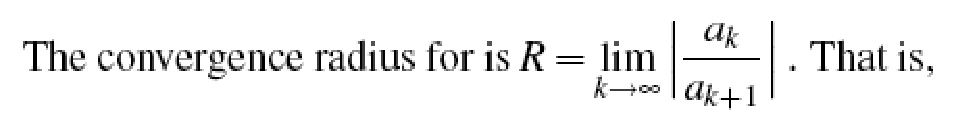
\includegraphics[width=0.55\textwidth]{latex}}}
	\subfigure[由Word软件生成的.doc格式行内公式]{\label{fig:subfig:word}
		\fbox{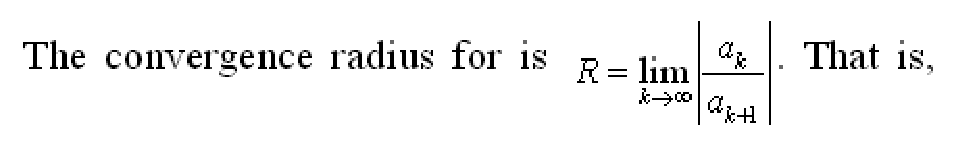
\includegraphics[width=0.55\textwidth]{word}}}
	\subfigure[由Word软件生成的.pdf格式行内公式]{\label{fig:subfig:pdf}
		\fbox{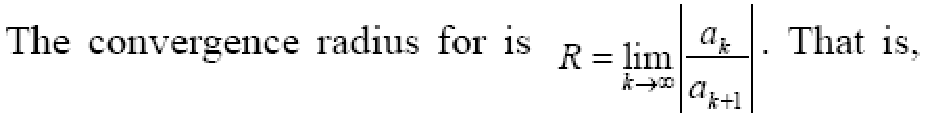
\includegraphics[width=0.55\textwidth]{pdf}}}

	\caption{由\LaTeX~和Word生成的3种行内公式屏显效果}\label{fig:hangju}
	\vspace{-1em}
\end{figure}

这三幅图分别为\LaTeX~和Word生成的行内公式屏显效果,从图中可看出,在\LaTeX~文本含有公式的行内,在正文与公式之间对接工整,行距不变;而在Word文本含有公式的行内,在正文与公式之间对接不齐,行距变大。因此从这一点来说,
\LaTeX~系统在数学公式的排版上具有很大优势。

\LaTeX~提供的行内公式最简单、最有效的方法是采用\TeX~本来的标记———开始和结束标记都写作\$,例如本段开始的例子可由下面的输入得到。
\verb|$f(x)=\int_{a}^{b}\frac{\sin{x}}{x}\mathrm{d}x$|

\section{行间公式}
位于两行之间的公式称为行间公式,每个公式都是一个单独的段落,例如
\[\int_a^b{f\left(x\right)\mathrm{d}x}=\lim_{\left\|\Delta{x_i}\right\|\to 0}\sum_i{f\left(\xi_i\right)\Delta{x_i}}\]
除人工编号外,\LaTeX~各种类型行间公式的标记见表\ref{tab:eqtag}。
\begin{table}[htbp]
	\caption{各种类型行间公式的标记}\label{tab:eqtag}
	\vspace{0.5em}\centering\zihao{5}
	\begin{tabularx}{\textwidth}{cll}
		\toprule
		         & 无编号                     & 自动编号                \\
		\midrule
		单行公式 & \verb|\begin{displaymath}... \end{displaymath}|    & \verb|\begin{equation}... \end{equation}| \\
		         & 或\verb|\[...\]| &                         \\
		多行公式 & \verb|\begin{eqnarray*}... \end{eqnarray*}|    & \verb|\begin{eqnarray}... \end{eqnarray}| \\
		\bottomrule
	\end{tabularx}
\end{table}

另外,在自动编号的某行公式行尾添加标签\verb|\nonumber|,可将该行转换为无编号形式。

行间多行公式需采用\verb|eqnarray|或\verb|eqnarray*|环境,它默认是一个列格式为\verb|rcl|的3列矩阵,并且中间列的字号要小一些,因此通常只将需要对齐的运算符号(通常为等号“=”)置于中间列。

\section{可自动调整大小的定界符}
若在左右两个定界符之前分别添加命令\verb|\left|和\verb|\right|,则定界符可根据所包围公式大小自动调整其尺寸,这可从式(\ref{nodelimiter})和式(\ref{delimiter})中看出。
\begin{equation}\label{nodelimiter}
	(\sum_{k=\frac12}^{N^2})
\end{equation}
\begin{equation}\label{delimiter}
	\left(\sum_{k=\frac12}^{N^2}\right)
\end{equation}
式(\ref{nodelimiter})和式(\ref{delimiter})是在\LaTeX~中分别输入如下代码得到的。
\begin{verbatim}
	(\sum_{k=\frac12}^{N^2})
	\left(\sum_{k=\frac12}^{N^2}\right)
\end{verbatim}
\verb|\left|和\verb|\right|总是成对出现的,若只需在公式一侧有可自动调整大小的定界符,则只要用“.”代替另一侧那个无需打印出来的定界符即可。

若想获得关于此部分内容的更多信息,可参见\href{http://tug.ctan.org/cgi-bin/ctanPackageInformation.py?id=voss-mathmode}{Math mode}文档的第8章“Brackets, braces and parentheses”。

\section{数学重音符号}
数学重音符号通常用来区分同一字母表示的不同变量,输入方法如下(需要调用\verb|amsmath|宏包):

\vspace{0.5em}\noindent\zihao{5}\begin{tabularx}{\textwidth}{Xc|Xc|Xc}
	\verb|\acute| & $\acute{a}$ & \verb|\mathring| & $\mathring{a}$           & \verb|\underbrace| & $\underbrace{a}$          \\
	\verb|\bar| & $\bar{a}$   & \verb|\overbrace| & $\overbrace{a}$          & \verb|\underleftarrow| & $\underleftarrow{a}$      \\
	\verb|\breve| & $\breve{a}$ & \verb|\overleftarrow| & $\overleftarrow{a}$      & \verb|\underleftrightarrow| & $\underleftrightarrow{a}$ \\
	\verb|\check| & $\check{a}$ & \verb|\overleftrightarrow| & $\overleftrightarrow{a}$ & \verb|\underline| & $\underline{a}$           \\
	\verb|\dddot| & $\dddot{a}$ & \verb|\overline| & $\overline{a}$           & \verb|\underrightarrow| & $\underrightarrow{a}$     \\
	\verb|\ddot| & $\ddot{a}$  & \verb|\overrightarrow| & $\overrightarrow{a}$     & \verb|\vec| & $\vec{a}$                 \\
	\verb|\dot| & $\dot{a}$   & \verb|\tilde| & $\tilde{a}$              & \verb|\widehat| & $\widehat{a}$             \\
	\verb|\grave| & $\grave{a}$ & \verb|\underbar| & $\underbar{a}$           & \verb|\widetilde| & $\widetilde{a}$           \\
	\verb|\hat| & $\hat{a}$
\end{tabularx}\vspace{0.5em}
\zihao{4} 当需要在字母$i$和$j$的上方添加重音符号时,为了去掉这两个字母顶上的小点,这两个字母应该分别改用\verb|\imath|和\verb|\jmath|。

如果遇到某些符号不知道该采用什么命令能输出它时,则可通过\href{http://detexify.kirelabs.org/classify.html}{Detexify$^2$网站}来获取符号命令。若用鼠标左键在此网页的方框区域内画出你所要找的符号形状,则会在网页右方列出和你所画符号形状相近的5个符号及其相对应的\LaTeX~输入命令。若所列出的符号中不包括你所要找的符号,还可通过点击“Select from the complete list!”以得分从低到高的顺序列出所有符号及其相对应的\LaTeX~输入命令。

最后,建议大家还以\href{http://tug.ctan.org/cgi-bin/ctanPackageInformation.py?id=voss-mathmode}{Math mode}这篇pdf文档作为主要参考。若要获得最为标准、美观的数学公式排版形式,可以查查文档中是否有和你所要的排版形式相同或相近的代码段,通过修改代码段以获得你所要的数学公式排版形式。


%%% !TEX encoding = UTF-8
\chapter{简要版帮助}
若您已很熟悉\LaTeX~的相关操作,建议阅读这份简要帮助说明。
\section{模板文件结构\label{sec:files}}
整个模板根目录的文件列表如下:
\begin{center}
	\begin{tabular}{|l|p{7.5cm}|l|}
		\hline
		HUNNUthesis.tex          &\TeX{}样例文件             & \textcolor{red}{{*}} \\
		\hline
		HUNNUthesis.cls&包含论文所使用的宏包和全文格式的定义。& \textcolor{red}{{*}} \\
		\hline
		HUNNUThesis.tex& 主文件,包含封面、扉页和其他章节的引用信息。& \textcolor{red}{{*}} \\
		\hline
		preface& 包含毕业设计论文的中英文摘要。& \textcolor{red}{{*}} \\
		\hline
		images& 包含封面用到的湖南师范大学Logo。& \textcolor{red}{{*}} \\
		\hline
		figures& 包含正文中所用到的图片。& \textcolor{red}{{*}} \\
		\hline
		body& 包含正文的所有章节。& \textcolor{red}{{*}} \\
		\hline
		appendix& 附件相关内容& \textcolor{red}{{*}} \\
		\hline
		appendix.tex & 作者的发表论文和参加科研情况说明& \textcolor{red}{{*}} \\
		\hline
		acknowledgements.tex&致谢文件& \textcolor{red}{{*}} \\
		\hline
		statement.tex&原创性说明和版权使用授权说明书。& \textcolor{red}{{*}} \\
		\hline
		hunnubib.bst             & 参考文献样式文件               & \textcolor{red}{{*}} \\
		\hline
		references/reference.bib & bib数据库                  & \textcolor{red}{{*}} \\
		\hline
		official\_documents& 学位论文的撰写格式和开题报告实施管理办法。& \\
		\hline
		clean.bat& 双击此文件,可以用来清理HUNNUThesis.tex在编译之后生成的所有附属文件,如后缀名为.aux,.log,.bak的文件。&  \\
		\hline
	\end{tabular}
\end{center}
注: \textcolor{red}{{*}} 表示\LaTeX{}模板必须的文件。
\subsection{文献引用}
将引文的bib数据库(默认文件名为reference.bib)放入模板根目录下的references文件夹,即可通过插入---文献引用自动产生引文。
\begin{itemize}
	\item 参考文献上标引用
	\begin{itemize}
		\item Journal:An article \upcite{ELIDRISSI94,MELLINGER96}。%参考文献上标
		\item An book \upcite{IEEE-1363,tex,companion}。%参考文献正常引用
		\item Conference:A conference \upcite{kocher99,DPMG,cnproceed}。
		\item Manual:A manual\upcite{NPB2}。
		\item MasterThesis:\upcite{zhubajie,metamori2004,shaheshang,FistSystem01}。
	\end{itemize}
	\item 参考文献正常引用
	\begin{itemize}
	\item Journal:An article \cite{ELIDRISSI94,MELLINGER96}。%参考文献上标
	\item An book \cite{IEEE-1363,tex,companion}。%参考文献正常引用
	\item Conference:A conference \cite{kocher99,DPMG,cnproceed}。
	\item Manual:A manual\cite{NPB2}。
	\item MasterThesis:\cite{zhubajie,metamori2004,shaheshang,FistSystem01}。
\end{itemize}
\end{itemize}
\subsection{伪代码实现}
\begin{algorithm}
	\caption{放进冰箱的大象}\label{算法实例}
	\begin{algorithmic}
		\REQUIRE 有一只大象
		\ENSURE 放进冰箱里
		\FOR {没有剩余的大象}
		\IF {大象比冰箱大}
		\STATE 把大象分割
		\ENDIF
		\ENDFOR
		\STATE 第一步
		\STATE 第二步
		\STATE 第三步
	\end{algorithmic}
	AAA\end{algorithm}
\subsection{代码展示}
可以把你的程序添加到附录里,展示自己的工作。
\begin{lstlisting}[language={[ANSI]C},
numbers=left,
numberstyle=\tiny,
basicstyle=\small\ttfamily,
stringstyle=\color{purple},
keywordstyle=\color{blue}\bfseries,
commentstyle=\color{olive},
directivestyle=\color{blue},
showstringspaces=false]
	#include <stdio.h>
	int main(int argc, char ** argv)
	{
		/*打印Hello,world*/
		printf("Hello, world!\n");
		
		return 0;
	}
\end{lstlisting}
\section{依赖}
HUNNUthesis依赖于以下宏包,这些宏包在常见的\LaTeX{}发行版中都包括,在安装使用之前,请确定你的\TeX{}发行版中都已正常安装这些宏包
\begin{table}[H]
	\centering
	\begin{tabular}{cccc}
\hline
{natbib} & {amsmath} & {amsfonts} & {amssymb} \\

{graphicx} & {subfigure} & {mathptmx} & {float} \\

{fontenc} & {booktabs} & {setspace} & {listings} \\

{xcolor} & {multirow} & {fancyhdr} & {etoolbox} \\

{tocloft} & {array} & {makecell} & {forloop} \\

{xstring} & {hyperref} & {cleveref} & {enumitem} \\

{algorithm} & {algorithmic} & {caption} & {ifthen} \\

{titlesec} & {ulem} & {amssymb} & {wasysym} \\

{flafter} & {booktabs} & {longtable} & {tabularx} \\

{setspace} & {subfigure} & {enumitem} & {calc } \\

{txfonts} & {bm} & {ntheorem} & {fancyvrb} \\

{xcolor} & {--} & {--} & {--} \\
\hline
	\end{tabular}
\end{table}
如果你尚未安装这些宏包,可以启动你的 \TeX{} 发行版的宏包管理器
来安装;或者到 \url{http://www.ctan.org} 上搜索下载并安装。
\section{基本设置}
\begin{enumerate}
	\item 论文正文所用图片搜索路径默认设置为模板根目录下的figures/。
	\item bib数据库默认设置为模板根目录下的references/reference.bib。 其中bib文件可由任意文献库管理软件自动生成
\end{enumerate}
\section{文字命令}
\subsection{常用命令}
\LaTeX 提供了一系列命令,用于修改字体、字号、数字等的呈现形式。
\subsubsection{字体}
ctex宏包及其文档类可直接使用以下六种字体:
\vspace{1em}\noindent\hrule
\begin{verbatim}
宋体: \songti       启用宋体  {\songti 宋体}。
黑体: \heiti        启用黑体  {\heiti 黑体}。
仿宋: \fangsong    启用仿宋   {\fangsong 仿宋}。
楷书: \kaishu       启用楷书   {\kaishu 楷书}。
隶书: \lishu        启用隶书  {\lishu 隶书}。
幼圆: \youyuan     启用幼圆   {\youyuan 幼圆}。
\end{verbatim}
\noindent\hrule\vspace{1em}

宋体:{\songti 宋体};黑体:{\heiti 黑体};仿宋:{\fangsong 仿宋};楷书:{\kaishu 楷书};隶书: {\lishu 隶书};幼圆: {\youyuan 幼圆}。
\subsubsection{字号}
{\bf 字号}%

\begin{center}
	\begin{tabular}{cccccccc}
		\toprule
		初号 & 小初 & 一号 & 小一 & 二号 & 小二 & 三号 & 小三 \\
		0    & -0   & 1    & -1   & 2    & -2   & 3    & -3   \\
		\hline
		四号 & 小四 & 五号 & 小五 & 六号 & 小六 & 七号 & 八号 \\
		4    & -4   & 5    & -5   & 6    & -6   & 7    & 8    \\
		\bottomrule
	\end{tabular}
\end{center}

\vspace{1em}\noindent\hrule
\begin{verbatim}
{\zihao{0}初号}; \dots {\zihao{4}四号};\dots 
\zihao{7}{七号} \zihao{4}
\end{verbatim}
\noindent\hrule\vspace{1em}

{\zihao{0}初号}; \dots {\zihao{4}四号};\dots \zihao{7}{七号}
\zihao{4}
%%% !TEX encoding = UTF-8
\addcontentsline{toc}{chapter}{结论}
\chapter*{结\quad 论}
结论单独作为一章排写,但不加章号。结论是毕业论文(设计)的总结,是整篇论文(设计)的归宿。要求精炼、准确地概述全文的主要观点:或自己赞成的观点、或自己反对的观点、或自己的创造性工作与新的见解及其意义和作用,还进一步提出需要讨论的问题和建议等。特别提醒这部分不是写你做毕业设计(论文)的感想,不是抒情。下面是一个分页符,可以另起一页

结论应是作者在学位论文研究过程中所取得的创新性成果的概要总结,不能与摘要混为一谈。
学位论文结论应包括论文的主要结果、创新点、展望三部分,在结论中应概括论文的核心观点,
明确、客观地指出本研究内容的创新性成果(含新见解、新观点、方法创新、技术创新、理论创新),并指出今后进一步在本研究方向进行研究工作的展望与设想。
对所取得的创新性成果应注意从定性和定量两方面给出科学、准确的评价,分(1)、(2)、(3)…条列出,宜用“提出了”、“建立了”等词叙述。

结论应是作者在学位论文研究过程中所取得的创新性成果的概要总结,不能与摘要混为一谈。
学位论文结论应包括论文的主要结果、创新点、展望三部分,在结论中应概括论文的核心观点,
明确、客观地指出本研究内容的创新性成果(含新见解、新观点、方法创新、技术创新、理论创新),并指出今后进一步在本研究方向进行研究工作的展望与设想。
对所取得的创新性成果应注意从定性和定量两方面给出科学、准确的评价,分(1)、(2)、(3)…条列出,宜用“提出了”、“建立了”等词叙述。

结论应是作者在学位论文研究过程中所取得的创新性成果的概要总结,不能与摘要混为一谈。
学位论文结论应包括论文的主要结果、创新点、展望三部分,在结论中应概括论文的核心观点,
明确、客观地指出本研究内容的创新性成果(含新见解、新观点、方法创新、技术创新、理论创新),并指出今后进一步在本研究方向进行研究工作的展望与设想。
对所取得的创新性成果应注意从定性和定量两方面给出科学、准确的评价,分(1)、(2)、(3)…条列出,宜用“提出了”、“建立了”等词叙述。

结论应是作者在学位论文研究过程中所取得的创新性成果的概要总结,不能与摘要混为一谈。
学位论文结论应包括论文的主要结果、创新点、展望三部分,在结论中应概括论文的核心观点,
明确、客观地指出本研究内容的创新性成果(含新见解、新观点、方法创新、技术创新、理论创新),并指出今后进一步在本研究方向进行研究工作的展望与设想。
对所取得的创新性成果应注意从定性和定量两方面给出科学、准确的评价,分(1)、(2)、(3)…条列出,宜用“提出了”、“建立了”等词叙述。
\end{verbatim}

\noindent\hrule\vspace{1em}

那么,编译的时候就只编译未加\%的一章,在这个例子中,即本章chapter1。

理论上,并不一定要把每章放在不同的文件中。但是这种自顶向下,分章节写作、编译的方法有利于提高效率,大大减少Debug过程中的编译时间,同时减小风险。
\section{参考文献生成方法}
\LaTeX~具有插入参考文献的能力。Google Scholar网站上存在兼容BibTeX的参考文献信息,通过以下几个步骤,可以轻松完成参考文献的生成。
\begin{itemize}
	\item 在\href{http://scholar.google.com/}{谷歌学术搜索}中,
	      点击\href{http://scholar.google.com/scholar_preferences?hl=en&as_sdt=0,5}{学术搜索设置}。
	\item 页面打开之后,在{\bf 文献管理软件}选项中选择{\bf 显示导入BibTeX的链接},单击保存设置,退出。
	\item 在谷歌学术搜索中检索到文献后,在文献条目区域单击导入BibTeX选项,页面中出现文献的引用信息。
	\item 将文献引用信息的内容复制之后,添加到references文件夹下的reference.bib中。
\end{itemize}
\section{编译注意事项}
\begin{enumerate}
	\item 由于模板使用UTF-8编码,所以源文件应该保存成UTF-8格式,否则可能出现中文字符无法识别的错误。
	      本模板中每一个.tex文件的文件的开头已经加上一行:\\
	      \verb|% !Mode:: "TeX:UTF-8"|\\
	      这样可以确保.tex文件默认使用UTF-8的格式打开。读者如果删去此行,很有可能会导致中文字符显示乱码。
	\item 建议采用以下编译方式:

	{\color{red}\heiti\bfseries XeLaTeX --> BibTeX --> XeLaTeX --> XeLaTeX}
\end{enumerate}
\section{系统要求}
TeX Live 2019或以上版本。使用推荐的TexStudio编辑器,可以完成文件的编辑和编译工作。
\section{\TeX~简介}
以下内容是milksea@bbs.ctex.org撰写的关于\TeX~的简单介绍,略有改动。
注意这不是一个入门教程,不讲\TeX~系统的配置安装,也不讲具体的\LaTeX~代码。
这里仅仅试图以一些只言片语来解释:
进入这个门槛之前新手应该知道的注意事项,以及遇到问题以后该去如何解决问题。
\subsection{什么是 \TeX/\LaTeX~,我是否应该选择它?}
\TeX~是最早由高德纳(Donald Knuth)教授创建的一门标记式宏语言,
用来排版科技文章,尤其擅长处理复杂的数学公式。\TeX~同时也是处理这一语言的排版软件。
\LaTeX~是 Leslie Lamport 在\TeX~基础上按内容/格式分离和模块化等思想建立的一集\TeX~上的格式。

\TeX~本身的领域是专业排版领域
但现在TeX/LaTeX也被广泛用于生成电子文档甚至幻灯片等,\TeX~语言的数学部分
偶尔也在其他一些地方使用。但注意\TeX~并不适用于文书处理(Microsoft Office 的领域,以前和现在都不是)。

选择使用\TeX/\LaTeX~的理由包括:
\begin{itemize}
	\item 免费软件;
	\item 专业的排版效果;
	\item 是事实上的专业数学排版标准;
	\item 广泛的西文期刊接收甚或只接收 LaTeX 格式的投稿;
	\item[] ……
\end{itemize}
不选择使用\TeX/\LaTeX~的理由包括:
\begin{itemize}
	\item 需要相当精力学习;
	\item 图文混合排版能力不够强;
	\item 仅在数学、物理、计算机等领域流行;
	\item 中文期刊的支持较差;
	\item[] ……
\end{itemize}

请尽量清醒看待网上经常见到的关于\TeX~与其他软件的优劣比较和口水战。在选择使用或离开之前,请先考虑
\TeX~的应用领域,想想它是否适合你的需要。
\subsection{我该用什么编辑器?}
编辑器功能有简有繁,特色不一,从简单的纯文本编辑器到繁复的 Emacs,因人而易。基本功能有语法高亮、方便编译预览就很好了,扩充功能和定制有无限的可能。初学者可以使用功能简单、使用方便的专用编辑器,如TexStudio、TeXWorks、Kile、WinEdt等,或者类似所见即所得功能的LyX;熟悉的人可以使用定制性更强的Notepad++、SciTE、Vim、Emacs 等。这方面的介绍很多,一开始不妨多试几种,找到最适合自己的才是最好的。

另外提醒一句,编辑器只是工作的助手,不必把它看得太重。
\subsection{我应该看什么\LaTeX~读物?}
这不是一个容易回答的问题,因为有许多选择,也同样有许多不合适的选择。
这里只是选出一个比较好的答案。更多更详细的介绍可以在版面和网上寻找(注意时效)。

近两年\TeX~的中文处理发展很快,目前没有哪本书在中文处理方面给出一个最新进展的合适综述,
因而下面的介绍也不主要考虑中文处理。

\begin{enumerate}
	\item 我能阅读英文。
	      \begin{enumerate}
		      \item 迅速入门:ltxprimer.pdf (LaTeX Tutorials: A Primer, India TUG)
		      \item 系统学习:A Guide to LaTeX, 4th Edition, Addison-Wesley
		            有机械工业出版社的影印版(《\LaTeX{}实用教程》)
		      \item 深入学习:要读许多书和文档,TeXbook 是必读的
		      \item 细节学习:去读你使用的每一个宏包的说明文档
		      \item 专题学习:阅读讲数学公式、图形、表格、字体等的专题文档
	      \end{enumerate}
	\item 我更愿意阅读中文。
	      \begin{enumerate}
		      \item 迅速入门:lnotes.pdf (LaTeX Notes, 1.20, Alpha Huang)
		      \item 系统学习:《\LaTeXe{}科技排版指南》,邓建松(电子版)
		            如果不好找,可以阅读《\LaTeXe~入门与提高》第二版,陈志杰等,或者 《\LaTeXe~完全学习手册》,胡伟
		      \item 深入学习:TeXbook0.pdf(特可爱原本,TeXbook 的中译,xianxian)
		      \item 具体问题释疑:CTeX-FAQ.pdf,\\
		            吴凌云,\url{http://www.ctex.org/CTeXFAQ}
	      \end{enumerate}
\end{enumerate}

遇见问题和解决问题的过程可以快速提高自己的技能,建议此时:
\begin{itemize}
	\item 利用Google搜索。
	\item 清楚,扼要地提出你的问题。
\end{itemize}

\subsection{什么知识会过时?什么不会?}
\TeX~是排版语言,也是广泛使用的软件,并且不断在发展中;
因此,总有一些东西会很快过时。作为学习\TeX~的人,
免不了要看各种各样的书籍、电子文档和网络论坛上的只言片语,
因此了解什么知识会迅速过时,什么知识不会是十分重要的。

最稳定的是关于Primitive \TeX~和Plain \TeX~的知识,也就是 Knuth
在他的《The TeXbook》中介绍的内容。因为\TeX~系统开发的初衷就是稳定性,要求今天的文档到很久以后仍可以得到完全相同的结果,
因此 Knuth 限定了他的\TeX~语言和相关实现的命令、语法。这些内容许多年来就没有多少变化,
在未来的一些年里也不会有什么变化。
Primitive \TeX~和 Plain \TeX~的知识主要包括 \TeX~排版的基本算法和原理,
盒子的原理,底层的 \TeX~命令等。其中技巧性的东西大多在宏包设计中,
初学者一般不会接触到很多;而基本原理则是常常被提到的,
譬如,\TeX~把一切排版内容作为盒子(box)处理。

相对稳定的是关于基本\LaTeXe~的知识,也包括围绕\LaTeXe~的一些核心宏包的知识。\LaTeXe~是自1993年以来的一个稳定的\LaTeX~版本,直到最近的一次修订(2005 年)都没有大的变动。\LaTeX~的下一个计划中的版本\LaTeX 3遥遥无期,在可预见的将来,\LaTeXe~不会过时。\LaTeXe~的知识是目前大部分\LaTeX~书籍的主体内容。关于\LaTeX~的标准文档类(article、report、book、letter、slide等),关于基本数学公式的输入,文档的章节层次,表格和矩阵,图表浮动体,LR 盒子与段落盒子……这些\LaTeX~的核心内容都是最常用的,相对稳定的。与\LaTeXe~相匹配的核心宏包,如graphics(x)、ifthen、fontenc、doc等,也同样是相对稳定的。还有一些被非常广泛应用的宏包,如amsmath系列,也可以看作是相对稳定的。

简单地说,关于基本\TeX/\LaTeX~的语言,都是比较稳定的。与之对应,实现或者支持\TeX/\LaTeX~语言的软件,包括在\TeX/\LaTeX~基础上建立的新的宏,都不大稳定。

容易过时的是关于第三方\LaTeX~宏包的知识、第三方\TeX~工具的知识,以及新兴\TeX~相关软件的知识等。\TeX~和\LaTeX~语言是追求稳定的;但无论是宏包还是工具,作为不断更新软件,它们是不稳定的。容易过时的技术很多,而且现在广泛地出现在几乎所有\LaTeX~文档之中,因此需要特别引起注意:宏包的过时的原因可能是宏包本身的升级换代带来了新功能或不兼容,也可能是同一功能的更新更好的宏包代替了旧的宏包。前者的典型例子比如绘图宏包PGF/TikZ,现在的2.00版功能十分强大,和旧的1.1x版相差很大,和更旧的0.x版本则几乎完全不同;后者的典型例子比如caption宏包先是被更新的caption2宏包代替,后来caption宏包更新又使得caption2 宏包完全过时。——安装更新的发行版可以避免使用过旧的宏包;认真阅读宏包自带的文档而不是搜索得到的陈旧片断可以避免采用过时的代码。

工具过时的主要原因也是升级换代和被其他工具替换。前者的典型例子是编辑器WinEdt在5.5以后的版本支持UTF-8编码,而旧版本不支持;后者的典型例子是中文字体安装工具从GBKFonts到xGBKFonts到FontsGen不断被取代。图形插入是一个在\TeX~实现、宏包与外围工具方面都更新很快的东西。在过去,最常用的输出格式是PS(PostScript)格式,因此插入的图像以EPS为主流。使用Dvips为主要输出工具,外围工具有GhostScript、bmeps等等,相关宏包有graphics等,相关文档如《\LaTeXe{} 插图指南》。

但凡提及“\LaTeX~只支持EPS图形”的,就是这个过时的时代的产物。事实上\TeX/\LaTeX~并不限定任何图形格式,只不过是当时的输出格式(PS)和工具(Dvips)对EPS情有独钟而已。后来 PDF 格式成为主流。pdf\TeX~、DVIPDFM、DVIPDFMx、XeTeX工具则主要支持PDF、PNG、JPG格式的图形,涉及一系列工具如ImageMagick、ebb等。

值得特别提出注意的就是,中文处理也一起是更新迅速、容易过时的部分。而且因为中文处理一直没有一个“官方”的“标准”做法,软件、工具、文档以及网上纷繁的笔记也就显得相当混乱。从八十年代开始的CCT系统、天元系统,到后来的CJK方式,到近来的XeTeX和LuaTeX 方式,中文处理的原理、软件、宏包、配置方式等都在不断变化中。
\section{免责声明}
本模板依据《湖南师范大学研究生学位论文的撰写格式》编写,适用于所有博士、硕士生的学位论文编写。然而,作者不保证本模板完全符合学校要求,也不对由此带来的风险和损失承担任何责任。
%%% !Mode:: "TeX:UTF-8"
\chapter{图片的插入方法}
\section{研究生毕业论文的插图规范}
图应有自明性。插图应与文字紧密配合,文图相符,内容正确。选图要力求精练,插图、照片应完整清晰。图中文字和数字等字号用宋体五号字。

机械工程图:采用第一角投影法,严格按照GB4457---GB131-83《机械制图》标准规定。

数据流程图、程序流程图、系统流程图等按GB1526-89标准规定。

电气图:图形符号、文字符号等应符合有关标准的规定。

流程图:必须采用结构化程序并正确运用流程框图。

对无规定符号的图形应采用该行业的常用画法。

坐标图的坐标线均用细实线,粗细不得超过图中曲线,有数字标注的坐标图,必须注明坐标单位。

照片图要求主题和主要显示部分的轮廓鲜明,便于制版。如用放大或缩小的复制品,必须清晰,反差适中。照片上应有表示目的物尺寸的标度。

引用文献图表必须标注出处。

\subsection{图题及图中说明}
每个图均应有图题(由图序和图名组成),图名在图序之后空两格排写。图序按章编排,如第1章第一个插图的图号为“图1-1”等。
图题置于图下,要求中文用宋体五号字,位置居中。有图注或其它说明时应置于图题之上。引用图应注明出处,在图题右上角加引用文献号。
图中若有分图时,分图题置于分图之下或图题之下,分图号用a)、b)等表示。

图中各部分说明应采用中文(引用的外文图除外)或数字项号,各项文字说明置于图题之上(有分图题者,置于分图题之上)。

\subsection{插图编排}
插图之前,文中必须有关于本插图的提示,如“见图1-1”、“如图1-1所示”等。插图与其图题为一个整体,不得拆开排写于两页。
插图处的该页空白不够排写该图整体时,则可将其后文字部分提前排写,将图移到次页。

\section{\LaTeX~中推荐使用的图片格式}
在\LaTeX~中应用最多的图片格式是EPS(Encapsulated PostScript)格式,它是一种专用的打印机描述语言,常用于印刷或打印输出。
EPS格式图片可通过多种方式生成,这里介绍一款功能强大的免费图片处理软件———\href{http://www.imagemagick.org/}{ImageMagick},
此软件可将其它格式图片转换为EPS格式图片,同时还可以锐化图片,使图片的局部清晰一些。

此软件对图片的格式转换操作都是在命令提示符(cmd.exe)中实现的,可以通过“开始$\to$运行$\to$输入cmd$\to$回车”或
“开始$\to$程序$\to$附件$\to$命令提示符”找到它。在命令提示符下,首先采用“盘符命令”或“cd命令”将当前目录改为待处理图片所在的目录,
在此目录下就可通过convert命令将图片转换为EPS格式,其命令的语法格式为

\indent\verb|convert [可选参数] 原文件名.原扩展名 新文件名.eps|.

若convert命令中无可选参数,则将原来的图片格式直接转换为EPS格式,对图片不进行任何处理,这也是最常用的方法。
也可以选用可选参数,可选参数有很多选择,但最常用的有如下两个:

\verb|-sharpen radius{xsigma}|———此参数用来锐化图片,一般用在图片像素不高,需要提高图片清晰度的情况下。其中radius只能为整数,
它用来确定转换命令采取哪一种锐化算法,我们可以只取radius为0;sigma为所采取算法的锐化度,它的取值为$0.1 - 3$之间的任意一个浮点数,
数值越大,锐化程度也越大,通常取为$0.1 - 3$之间;x在参数中为分隔符。
\verb|-resize geometry|———此参数用来改变图片的大小,若图片的存储空间过大,可通过此命令缩小图片尺寸,但同时也将导致图片像素降低,
其具体用法请参见\href{http://www.imagemagick.org/script/command-line-options.php#resize}{-resize geometry的官方说明}。

除此之外,一些文字处理软件和科学计算软件也支持生成EPS格式的文件,请使用“另存为”功能查看某款软件是否能够将图片以EPS格式的形式保存。

\section{单张图片的插入方法}
单张图片独自占一行的插入形式如图\ref{fig:xml}所示。
\begin{figure}[htbp]
	\centering
	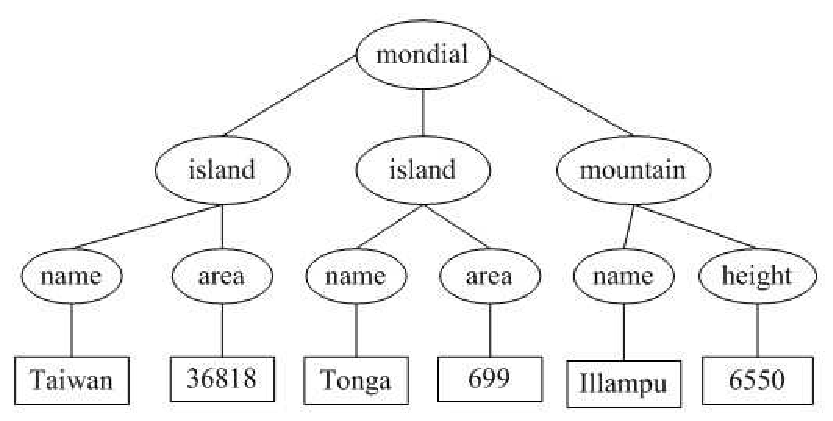
\includegraphics[width=0.4\textwidth]{XML}
	\caption{树状结构}\label{fig:xml}
	\vspace{\baselineskip}
\end{figure}


其插入图片的代码及其说明如下。
\vspace{1em}\noindent\hrule
\begin{verbatim}
	\begin{figure}[htbp]
		\centering
		\includegraphics[width=0.4\textwidth]{文件名(.eps)}
		\caption{标题}\label{标签名(通常为 fig:labelname)}
		\vspace{\baselineskip} %表示图与正文空一行
	\end{figure}
\end{verbatim}

\noindent\hrule

\begin{verbatim}
figure环境的可选参数[htbp]表示浮动图形所放置的位置,h (here)
表示当前位置,t (top)表示页芯顶部,b (bottom)表示页芯底部,
p (page)表示单独一页。在Word等软件中,图片通常插入到当前位置,
如果当前页的剩余空间不够,图片将被移动到下一页,当前页就会出现
很大的空白,其人工调整工作非常不便。由LaTeX提供的浮动图片功能,
总是会按h->t->b->p的次序处理选项中的字母,自动调整图片的位置,
大大减轻了工作量。\centering命令将后续内容转换成每行皆居中的格式。
"\includegraphics"的可选参数用来设置图片插入文中的水平宽度,
一般表示为正文宽度(\textwidth)的倍数。	\caption命令可选
参数“标签名”为英文形式,一般不以图片或表格的数字顺序作为标签,
而应包含一定的图片或表格信息,以便于文中引用(若图片、表格、公
式、章节和参考文献等在文中出现的先后顺序发生了变化,其标注序号
及其文中引用序号也会跟着发生变化,这一点是Word等软件所不能做到
的)。另外,图题或表题并不会因为分页而与图片或表格体分置于两页,
章节等各级标题也不会置于某页的最底部,LaTeX系统会自动调整它们在
正文中的位置,这也是Word等软件所无法匹敌的。\vspace将产生一定
高度的竖直空白,必选参数为负值表示将后续文字位置向上提升,参数
值可自行调整。em为长度单位,相当于大写字母M的宽度。
\vspace{\baselineskip} 表示图与正文空一行。
引用方法:“见图\ref{fig:figname}”、“如图\ref{fig:figname}所示”等。
\end{verbatim}

\noindent\hrule\vspace{1em}

若需要将2张及以上的图片并排插入到一行中,则需要采用\verb|minipage|环境,如图\ref{fig:dd}和图\ref{fig:ds}所示。
\begin{figure}[htbp]
	\centering
	\begin{minipage}{0.4\textwidth}
		\centering
		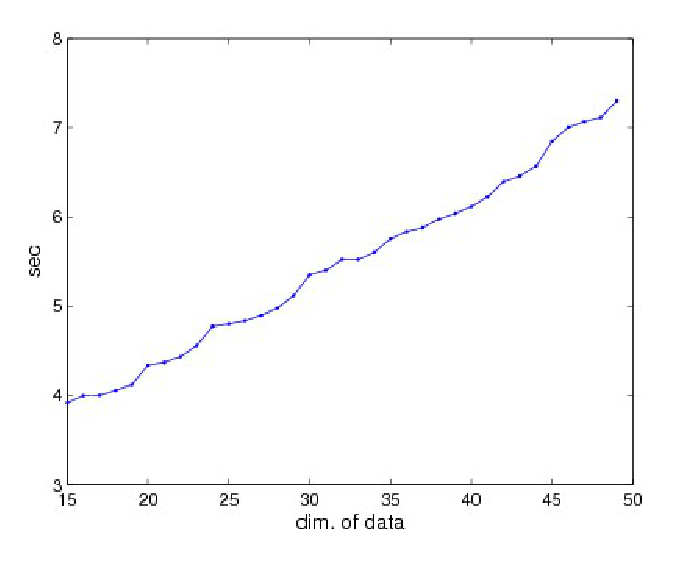
\includegraphics[width=\textwidth]{dataDimensions}
		\caption{数据维数的变化}\label{fig:dd}
	\end{minipage}
	\begin{minipage}{0.4\textwidth}
		\centering
		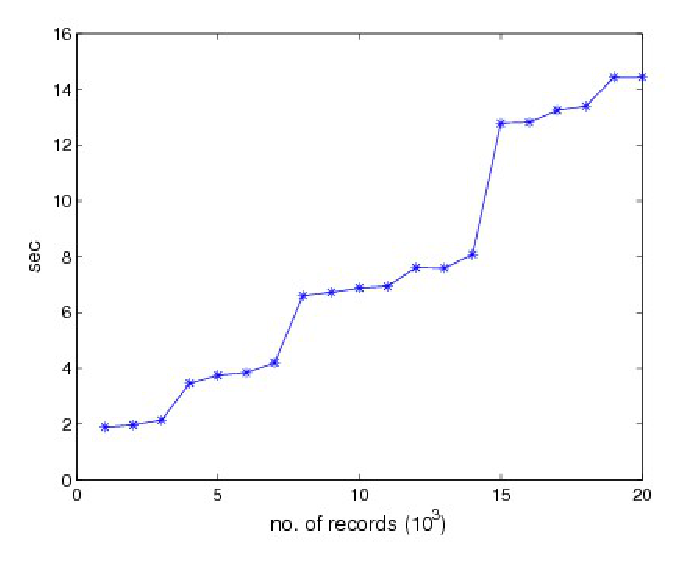
\includegraphics[width=\textwidth]{dataSize}
		\caption{数据规模的变化}\label{fig:ds}
	\end{minipage}
	\vspace{\baselineskip}
\end{figure}

其代码如下所示。

\vspace{1em}\noindent\hrule
\begin{verbatim}
	\begin{figure}[htbp]
		\centering
		\begin{minipage}{0.4\textwidth}
			\centering
			\includegraphics[width=\textwidth]{文件名}
			\caption{标题}\label{fig:f1}
		\end{minipage}
		\begin{minipage}{0.4\textwidth}
			\centering
			\includegraphics[width=\textwidth]{文件名}
			\caption{标题}\label{fig:f2}
		\end{minipage}\vspace{\baselineskip}
	\end{figure}
\end{verbatim}

\noindent\hrule

\begin{verbatim}
minipage环境的必选参数用来设置小页的宽度,若需要在一行中插入
n个等宽图片,则每个小页的宽度应略小于(1/n)\textwidth。
\end{verbatim}

\noindent\hrule

\section{具有子图的图片插入方法}
图中若含有子图时,需要调用subfigure宏包, 如图\ref{fig:subfig}所示。
\begin{figure}[htbp]
	\centering
	\subfigure[Data Dimensions]{\label{fig:subfig:datadim}
		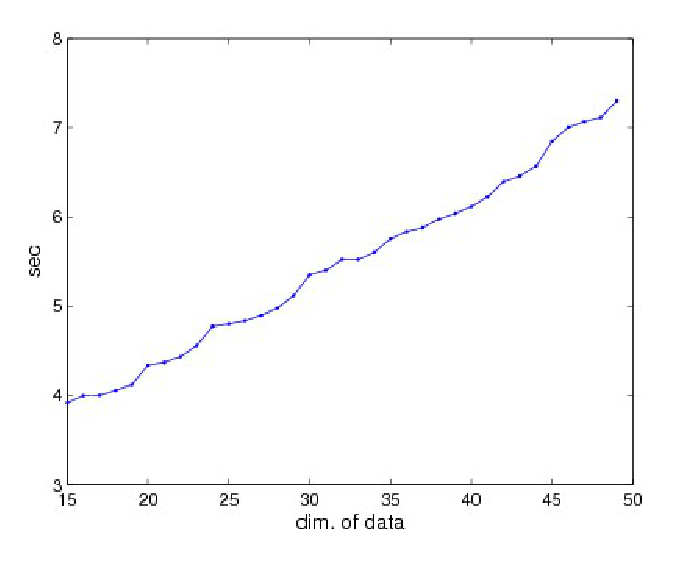
\includegraphics[width=0.4\textwidth]{dataDimensions}}
	\subfigure[Data Size]{\label{fig:subfig:datasize}
		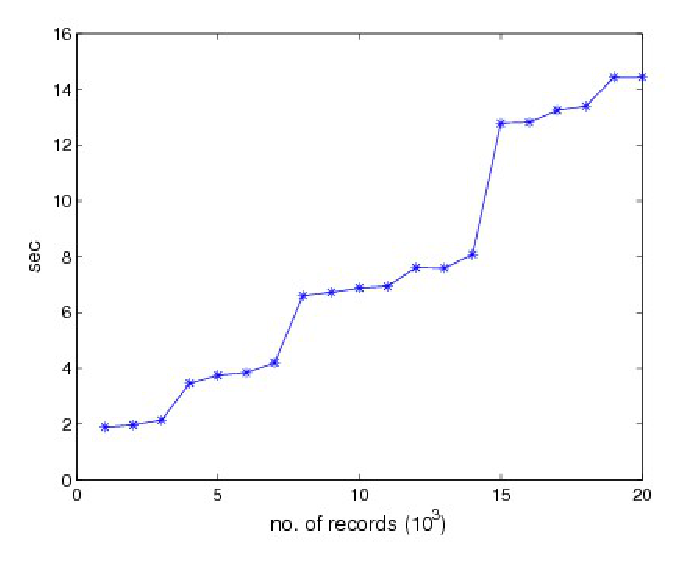
\includegraphics[width=0.4\textwidth]{dataSize}}
	\caption{Scalability of data}\label{fig:subfig}
	\vspace{\baselineskip}
\end{figure}

其代码及其说明如下。
\vspace{1em}\noindent\hrule

\begin{verbatim}
	\begin{figure}[htbp]
		\centering
		\subfigure[第1个子图标题]{
			\label{第1个子图标签(通常为 fig:subfig1:subsubfig1)}
			\includegraphics[width=0.4\textwidth]{文件名}}
		\subfigure[第2个子图标题]{
			\label{第2个子图标签(通常为 fig:subfig1:subsubfig2)}
			\includegraphics[width=0.4\textwidth]{文件名}}
		\caption{总标题}\label{总标签(通常为 fig:subfig1)}
		\vspace{\baselineskip}
	\end{figure}
\end{verbatim}

\noindent\hrule

\begin{verbatim}
	子图的标签实际上可以随意设定,只要不重复就行。但为了更好的
	可读性,我们建议fig:subfig:subsubfig格式命名,这样我们
	从标签名就可以知道这是一个子图引用。引用方法:总图的引用方
	法同本章第1节,子图的引用方法用\ref{fig:subfig:subsubfig}
	来代替。
\end{verbatim}

\noindent\hrule\vspace{1em}

子图的引用示例:如图\ref{fig:subfig:datadim}和图\ref{fig:subfig:datasize}所示。

若想获得插图方法的更多信息,参见网络上的\href{ftp://ftp.tex.ac.uk/tex-archive/info/epslatex.pdf}{Using Imported Graphics in \LaTeX~ and pdf\LaTeX~}文档。
%%% !Mode:: "TeX:UTF-8"
\chapter{表格的绘制方法}
\section{研究生毕业设计论文的绘表规范}
表应有自明性。表格不加左、右边线。表的编排建议采用国际通行的三线表。表内中文书写使用宋体五号字。

每个表格之上均应有表题(由表序和表名组成)。表序一般按章编排,如第1章第一个插表的序号为“表1-1”等。表序与表名之间空两格,
表名使用中文五号字,居中。表名中不允许使用标点符号,表名后不加标点。
表头设计应简单明了,尽量不用斜线。表头中可采用化学,物理量等专业符号。

全表如用同一单位,则将单位符号移至表头右上角,加圆括号。
表中数据应准确无误,书写清楚。数字空缺的格内加横线“-”(占2个数字宽度)。表内文字或数字上、下或左、右相同时,
采用通栏处理方式,不允许用“〃”、“同上”之类的写法。

表内文字使用宋体五号字,垂直居中书写,起行空一格、转行顶格、句末不加标点。
如某个表需要转页接排,在随后的各页上应重复表的编号。编号后加“(续表)”,表题可省略。续表应重复表头。
表格绘制完成之后,与正文空一行。

\section{普通表格的绘制方法}
表格应具有三线表格式,因此需要调用booktabs宏包,其标准格式如表\ref{tab:table1}所示。
\begin{table}[htbp]
	\caption{符合研究生毕业论文绘图规范的表格}\label{tab:table1}
	\vspace{0.5em}\centering\zihao{5}
	\begin{tabular}{ccccc}
		\toprule[1.5pt]
		$D$(in) & $P_u$(lbs) & $u_u$(in) & $\beta$ & $G_f$(psi.in) \\
		\midrule[1pt]
		5       & 269.8      & 0.000674  & 1.79    & 0.04089       \\
		10      & 421.0      & 0.001035  & 3.59    & 0.04089       \\
		20      & 640.2      & 0.001565  & 7.18    & 0.04089       \\
		5       & 269.8      & 0.000674  & 1.79    & 0.04089       \\
		10      & 421.0      & 0.001035  & 3.59    & 0.04089       \\
		20      & 640.2      & 0.001565  & 7.18    & 0.04089       \\
		5       & 269.8      & 0.000674  & 1.79    & 0.04089       \\
		10      & 421.0      & 0.001035  & 3.59    & 0.04089       \\
		20      & 640.2      & 0.001565  & 7.18    & 0.04089       \\
		5       & 269.8      & 0.000674  & 1.79    & 0.04089       \\
		10      & 421.0      & 0.001035  & 3.59    & 0.04089       \\
		20      & 640.2      & 0.001565  & 7.18    & 0.04089       \\
		\bottomrule[1.5pt]
	\end{tabular}
	\vspace{\baselineskip}
\end{table}

其绘制表格的代码及其说明如下。
\vspace{2em}\noindent\hrule

\begin{verbatim}
	\begin{table}[htbp]
		\caption{表标题}\label{标签名(通常为 tab:tablename)}
		\vspace{0.5em}\centering\zihao{5}
		\begin{tabular}{cc...c}
			\toprule[1.5pt]
			表头第1个格   & 表头第2个格   & ... & 表头第n个格  \\
			\midrule[1pt]
			表中数据(1,1) & 表中数据(1,2) & ... & 表中数据(1,n)\\
			表中数据(2,1) & 表中数据(2,2) & ... & 表中数据(2,n)\\
			表中数据(3,1) & 表中数据(3,2) & ... & 表中数据(3,n)\\
			表中数据(4,1) & 表中数据(4,2) & ... & 表中数据(4,n)\\
			...................................................\\
			表中数据(m,1) & 表中数据(m,2) & ... & 表中数据(m,n)\\
			\bottomrule[1.5pt]
		\end{tabular}
		\vspace{\baselineskip}
	\end{table}
\end{verbatim}

\noindent\hrule

\begin{verbatim}
	table环境是一个将表格嵌入文本的浮动环境。\zihao{5}命令将表
	格的字号设置为五号字(10.5pt),在绘制表格结束退出时,不需
	要将字号再改回为\zihao{-4},正文字号默认为小四号字(12pt)。
	tabular环境的必选参数由每列对应一个格式字符所组成:c表示居
	中,l表示左对齐,r表示右对齐,其总个数应与表的列数相同。此
	外,@{文本}可以出现在任意两个上述的列格式之间,其中的文本
	将被插入每一行的同一位置。表格的各行以\\分隔,同一行的各列
	则以&分隔。\toprule、\midrule和\bottomrule三个命令是由booktabs
	宏包提供的,其中\toprule和\bottomrule分别用来绘制表格的第一
	条(表格最顶部)和第三条(表格最底部)水平线,\midrule用来
	绘制第二条(表头之下)水平线,且第一条和第三条水平线的线宽
	为1.5pt,第二条水平线的线宽为1pt。
	引用方法:“如表\ref{tab:tablename}所示”。
\end{verbatim}

\noindent\hrule
\section{长表格的绘制方法}
长表格是当表格在当前页排不下而需要转页接排的情况下所采用的一种表格环境。若长表格仍按照普通表格的绘制方法来获得,
其所使用的\verb|table|浮动环境无法实现表格的换页接排功能,表格下方过长部分会排在表格第1页的页脚以下。为了能够实现长表格的转页接排功能,
需要调用longtable宏包,由于长表格是跨页的文本内容,因此只需要单独的\verb|longtable|环境,所绘制的长表格的格式如表\ref{tab:table2}所示。

此长表格\ref{tab:table2}第2页的标题“编号(续表)”和表头是通过代码自动添加上去的,无需人工添加,若表格在页面中的竖直位置发生了变化,长表格在第2页
及之后各页的标题和表头位置能够始终处于各页的最顶部,也无需人工调整,\LaTeX~系统的这一优点是Word等软件所无法企及的。

下段内容是为了让下面的长表格分居两页,看到表标题“编号(续表)”的效果。摘录于《你若安好,便是晴天 -- 林徽因传》片段:

她叫林徽因,出生于杭州,是许多人梦中期待的白莲。她在雨雾之都伦敦,发生过一场空前绝后的康桥之恋。她爱过三个男子,爱得清醒,也爱得平静。徐志摩为她徜徉在康桥,深情地等待一场旧梦可以归来。梁思成与她携手走过千山万水,为完成使命而相约白头。金岳霖为她终身不娶,痴心不改地守候一世。可她懂得人生飘忽不定,要学会随遇而安。
真正的平静,不是避开车马喧嚣,而是在心中修篱种菊。尽管如流往事,每一天都涛声依旧,只要我们消除执念,便可寂静安然。愿每个人在纷呈世相中不会迷失荒径,可以端坐磐石上,醉倒落花前。
如果可以,请让我预支一段如莲的时光,哪怕将来某一天加倍偿还。这个雨季会在何时停歇,无从知晓。但我知道,你若安好,便是晴天。

\zihao{5}\begin{longtable}{ccc}
	\caption{湖南大学各学院名称一览}\label{tab:table2}
	\vspace{0.5em}                                                                                   \\
	\toprule[1.5pt] 学院名称 & 网址                                                  & 联系电话      \\ \midrule[1pt]
	\endfirsthead
	\multicolumn{3}{c}{表\thetable(续表)}\vspace{0.5em}                                           \\
	\toprule[1.5pt] 学院名称 & 网址                                                  & 联系电话      \\ \midrule[1pt]
	\endhead
	\bottomrule[1.5pt]
	\endfoot
	机械与运载工程学院       & \url{http://mve.hnu.cn/}                              & 88822826      \\
	电气与信息工程学院       & \url{http://eeit.hnu.cn/}                             & 27404775      \\
	电子信息工程学院         & \url{http://www.tju.edu.cn/seie}                      & 27406956      \\
	电气与自动化工程学院     & \url{http://www2.tju.edu.cn/colleges/automate/}       & 27405477      \\
	建筑工程学院             & \url{http://www2.tju.edu.cn/colleges/civil/}          & 27404072      \\
	化工学院                 & \url{http://chemeng.tju.edu.cn/}                      & 27403389      \\
	材料科学与工程学院       & \url{http://mse.tju.edu.cn}                           & 27406693      \\
	建筑学院                 & \url{http://hgw022072.chinaw3.com/}                   & 27402724-2111 \\
	求是学部                                                                                         \\
	管理与经济学部           & \url{ http://sm.tju.edu.cn}                           & 27403423      \\
	理学院                   & \url{ http://www.tju.edu.cn/science/}                 & 27404118      \\
	文法学院                 & \url{ http://www2.tju.edu.cn/colleges/sociology/new/} & 27403691      \\
	信息科学与工程学院       & \url{http://ccc.hnu.cn/}                              & 88821907      \\
	马克思主义学院           & \url{http://www2.tju.edu.cn/colleges/marxism/}        & 27405348      \\
	环境科学与工程学院       & \url{http://www.tju.edu.cn/see}                       & 87402072      \\
	药物科学与技术学院       & \url{http://www2.tju.edu.cn/colleges/pharmtier/}      & 87401830      \\
	教育学院                 & \url{http://soe.tju.edu.cn/}                          & 27401028      \\
	职业技术教育学院         & \url{http://202.113.0.248:8888}                                       \\
	继续教育学院             & \url{http://aectu.tju.edu.cn/}                        & 27406298      \\
	仁爱学院                 & \url{http://www.tjrac.edu.cn/}                        & 68579990      \\
	农业与生物工程学院       & \url{http://202.113.13.169/site/nongxueyuan/}         & 87402171      \\
	国际教育学院             & \url{http://www.ietju.com/}                           & 27406147      \\
	网络教育学院             & \url{http://www.etju.com/}                            & 27426952      \\
\end{longtable}
\zihao{4}
\vspace{\baselineskip}

绘制长表格的代码及其说明如下。
\vspace{1em}\noindent\hrule

\begin{verbatim}
	\zihao{5}\begin{longtable}{cc...c}
		\caption{表标题}\label{标签名(通常为 tab:tablename)}\\
		\toprule[1.5pt] 表头第1个格 & 表头第2个格 & ... & 表头第n个格\\
		 \midrule[1pt]
		\endfirsthead
		\multicolumn{n}{c}{表\thetable(续表)}\vspace{0.5em}\\
		\toprule[1.5pt] 表头第1个格 & 表头第2个格 & ... & 表头第n个格\\
		 \midrule[1pt]
		\endhead
		\bottomrule[1.5pt]
		\endfoot
		表中数据(1,1) & 表中数据(1,2) & ... & 表中数据(1,n)\\
		表中数据(2,1) & 表中数据(2,2) & ... & 表中数据(2,n)\\
		...................................................\\
		表中数据(m,1) & 表中数据(m,2) & ... & 表中数据(m,n)\\
	\end{longtable}\xiaosi
\end{verbatim}

\noindent\hrule
\begin{verbatim}
	在绘制长表格的前面留出一个空白行,并在第2行的一开始全局定
	义长表格的字号为五号字,这样能够保证长表格之前段落的行距
	保持不变。在绘制长表格结束后,需要\zihao{-4}命令重新将字号
	改为小四号字。\endhead之前的文字描述的是第2页及其之后各
	页的标题或表头;\endfirsthead之前的文字描述的是第1页
	的标题和表头,若无此命令,则第1页的表头和标题由\endhead
	命令确定;同理,\endfoot之前的文字描述的是除最后一页之
	外每页的表格底部内容;\endlastfoot之前的文字描述的是最
	后一页的表格底部内容,若无此命令,则最后一页的表格底部内
	容由\endfoot命令确定;由于规范中长表格每页底部内容均相
	同(水平粗线),因此模板中没有用到\endlastfoot命令。
\end{verbatim}

\noindent\hrule
\section{列宽可调表格的绘制方法}
论文中能用到列宽可调表格的情况共有两种:一种是当插入的表格某一单元格内容过长以至于一行放不下的情况,
另一种是当对公式中首次出现的物理量符号进行注释的情况。这两种情况都需要调用tabularx宏包。下面将分别对这两种情况下可调表格的绘制方法进行阐述。
\subsection{表格内某单元格内容过长的情况}
首先给出这种情况下的一个例子如表\ref{tab:table3}所示。
\begin{table}[htbp]
	\caption{最小的三个正整数的英文表示法}\label{tab:table3}
	\vspace{0.5em}\zihao{5}
	\begin{tabularx}{\textwidth}{llX}
		\toprule[1.5pt]
		Value & Name  & Alternate names, and names for sets of the given size                                                                                           \\\midrule[1pt]
		1     & One   & ace, single, singleton, unary, unit, unity                                                                                                      \\
		2     & Two   & binary, brace, couple, couplet, distich, deuce, double, doubleton, duad, duality, duet, duo, dyad, pair, snake eyes, span, twain, twosome, yoke \\
		3     & Three & deuce-ace, leash, set, tercet, ternary, ternion, terzetto, threesome, tierce, trey, triad, trine, trinity, trio, triplet, troika, hat-trick     \\\bottomrule[1.5pt]
	\end{tabularx}
	\vspace{\baselineskip}
\end{table}
绘制这种表格的代码及其说明如下。
\vspace{1em}\noindent\hrule
\begin{verbatim}
	\begin{table}[htbp]
		\caption{表标题}\label{标签名(通常为 tab:tablename)}
		\vspace{0.5em}\zihao{5}
		\begin{tabularx}{\textwidth}{l...X...l}
			\toprule[1.5pt]
			表头第1个格   & ... & 表头第X个格   & ... & 表头第n个格  \\
			\midrule[1pt]
			表中数据(1,1) & ... & 表中数据(1,X) & ... & 表中数据(1,n)\\
			表中数据(2,1) & ... & 表中数据(2,X) & ... & 表中数据(2,n)\\
			.........................................................\\
			表中数据(m,1) & ... & 表中数据(m,X) & ... & 表中数据(m,n)\\
			\bottomrule[1.5pt]
		\end{tabularx}
		\vspace{\baselineskip}
	\end{table}
\end{verbatim}

\noindent\hrule
\begin{verbatim}
	tabularx环境共有两个必选参数:第1个参数用来确定表格的总宽
	度,这里取为排版表格能达到的最大宽度——正文宽度\textwidth;
	第2个参数用来确定每列格式,其中标为X的项表示该列的宽度可调,
	其宽度值由表格总宽度确定。标为X的列一般选为单元格内容过长而
	无法置于一行的列,这样使得该列内容能够根据表格总宽度自动分行。
	若列格式中存在不止一个X项,则这些标为X的列的列宽相同,因此,
	一般不将内容较短的列设为X。标为X的列均为左对齐,因此其余列一
	般选为l(左对齐),这样可使得表格美观,但也可以选为c或r。
\end{verbatim}

\noindent\hrule
\subsection{对物理量符号进行注释的情况}
为使得对公式中物理量符号注释的转行与破折号“———”后第一个字对齐,此处最好采用表格环境。此表格无任何线条,左对齐,
且在破折号处对齐,一共有“式中”二字、物理量符号和注释三列,表格的总宽度可选为文本宽度,因此应该采用\verb|tabularx|环境。
由\verb|tabularx|环境生成的对公式中物理量符号进行注释的公式如式(\ref{eq:1})所示。
%\vspace*{10pt}

\begin{equation}\label{eq:1}
	\ddot{\boldsymbol{\rho}}-\frac{\mu}{R_{t}^{3}}\left(3\mathbf{R_{t}}\frac{\mathbf{R_{t}\rho}}{R_{t}^{2}}-\boldsymbol{\rho}\right)=\mathbf{a}
\end{equation}

\begin{tabularx}{\textwidth}{@{}l@{\quad}r@{———}X@{}}
	式中 & $\bm{\rho}$        & 追踪飞行器与目标飞行器之间的相对位置矢量; \\
	     & $\bm{\ddot{\rho}}$ & 追踪飞行器与目标飞行器之间的相对加速度;   \\
	     & $\mathbf{a}$       & 推力所产生的加速度;                       \\
	     & $\mathbf{R_t}$     & 目标飞行器在惯性坐标系中的位置矢量;       \\
	     & $\omega_{t}$       & 目标飞行器的轨道角速度;                   \\
	     & $\mathbf{g}$       & 重力加速度。
\end{tabularx}
\vspace{\wordsep}

其中生成注释部分的代码及其说明如下。

\vspace{1em}\noindent\hrule

\begin{verbatim}
	\begin{tabularx}{\textwidth}{@{}l@{\quad}r@{— — —}X@{}}
		式中 & symbol-1 & symbol-1的注释内容;\\
		& symbol-2 & symbol-2的注释内容;\\
		.............................;\\
		& symbol-m & symbol-m的注释内容。
	\end{tabularx}\vspace{\wordsep}
\end{verbatim}

\noindent\hrule

\begin{verbatim}
	tabularx环境的第1个参数选为正文宽度,第2个参数里面各个符号
	的意义为:第1个@{}表示在“式中”二字左侧不插入任何文本,
	“式中”二字能够在正文中左对齐,若无此项,则“式中”二字左
	侧会留出一定的空白;@{\quad}表示在“式中”和物理量符号间插
	入一个空铅宽度的空白;@{— — —}实现插入破折号的功能,它
	由三个1/2的中文破折号构成;第2个@{}表示在注释内容靠近正文
	右边界的地方能够实现右对齐。
\end{verbatim}

\noindent\hrule\vspace{1em}

由此方法生成的注释内容应紧邻待注释公式并置于其下方,因此不能将代码放入\verb|table|浮动环境中。但此方法不能实现自动转页接排,
可能会在当前页剩余空间不够时,全部移动到下一页而导致当前页出现很大空白。因此在需要转页处理时,还请您手动将需要转页的代码放入一个
新的\verb|tabularx|环境中,将原来的一个\verb|tabularx|环境拆分为两个\verb|tabularx|环境。

若想获得绘制表格的更多信息,参见网络上的\href{http://www.tug.org/pracjourn/2007-1/mori/}{Tables in \LaTeX~e: Packages and Methods}文档。
%%% !Mode:: "TeX:UTF-8"
\chapter{数学公式的输入方法}
湖南师范大学研究生论文有关公式、数字、年代、符号的书写要求:
\begin{itemize}
	\item 年份一概写全数。例:1998年不能写成98年。
	\item 分数、世纪、年代均以阿拉伯数字表示。例:三分之二写成2/3;二十世纪九十年代写成20世纪90年代。
	\item 公式均需标注公式号,公式号用圆括号,阿拉伯数字表示,按章编排。
	\item 论文中的物理量、量纲及符号等均采用国际标准(SI)和国家标准(GB)。
\end{itemize}
\section{研究生毕业设计论文的公式规范}
论文中的公式应另起行,原则上应居中书写,与周围文字留有足够的空间区分开。
若公式前有文字(如“解”、“假定”等),文字空两格写,公式仍居中写。公式末不加标点。

公式应标注序号,并将序号置于括号内。 公式序号按章编排,如第1章第一个公式序号为“(1-1)”。公式的序号右端对齐。

公式较长时最好在等号“=”处转行,如难实现,则可在$+$、$-$、$\times$、$\div$运算符号处转行,转行时运算符号仅书写于转行式前,不重复书写。

文中引用公式时,一般用“见式(1-1)”或“由公式(1-1)”。

公式中用斜线表示“除”的关系时应采用括号,以免含糊不清,如$a/(b\cos x)$。通常“乘”的关系在前,如$a\cos x/b$而不写成$(a/b)\cos x$。

不能用文字形式表示等式,如:$\textnormal{刚度}=\frac{{\textnormal{受力}}}{{\textnormal{受力方向的位移}}}$。

对于数学公式的输入方法,网络上有一个比较全面权威的文档{\bf{\href{http://tug.ctan.org/cgi-bin/ctanPackageInformation.py?id=voss-mathmode}{Math mode}}}请大家事先大概浏览一下。下面将对学位论文中主要用到的数学公式排版形式进行阐述。

\section{生成\LaTeX~数学公式的两种方法}
对于先前没有接触过\LaTeX~的人来说,编写\LaTeX~数学公式是一件很繁琐的事,尤其是对复杂的数学公式来说,更可以说是一件难以完成的任务。
实际上,生成\LaTeX~数学公式有两种较为简便的方法,一种是基于MathType数学公式编辑器的方法,另一种是基于MATLAB商业数学软件的方法,
下面将分别对这两种数学公式的生成方法作一下简单介绍。

\subsection{基于MathType软件的数学公式生成方法}
MathType是一款功能强大的数学公式编辑器软件,能够用来在文本环境中插入Windows OLE图形格式的复杂数学公式,所以应用比较普遍。但此软件只有30天的试用期,之后若再继续使用则需要付费购买才行。网络上有很多破解版的MathType软件可供下载免费使用,
笔者推荐下载安装版本号在6.5之上的中文破解版。

在安装好MathType之后,若在输入窗口中编写数学公式,复制到剪贴板上的仍然是图形格式的对象。
若希望得到可插入到\LaTeX~编辑器中的文本格式对象,则需要对MathType软件做一下简单的设置:在MathType最上排的按钮中依次选择“参数选项
$\to$转换”,在弹出的对话窗中选中“转换到其它语言(文字):”,在转换下拉框中选择“Tex——LaTeX 2.09 and later”,并将对话框最下方的两个复选框全部勾掉,点击确定,这样,再从输入窗口中复制出来的对象就是文本格式的了,就可以直接将其粘贴到\LaTeX~
编辑器中了。按照这种方法生成的数学公式两端分别有标记\verb|\[|和标记\verb|\]|,在这两个标记之间才是真正的数学公式代码。

若希望从MathType输入窗口中复制出来的对象为图形格式,则只需再选中“公示对象(Windows OLE图形)”即可。

\subsection{基于MATLAB软件的数学公式生成方法}
MATLAB是矩阵实验室(Matrix Laboratory)的简称,是美国MathWorks公司出品的商业数学软件。它是当今科研领域最常用的应用软件之一,
具有强大的矩阵计算、符号运算和数据可视化功能,是一种简单易用、可扩展的系统开发环境和平台。

MATLAB中提供了一个latex函数,它可将符号表达式转化为\LaTeX~数学公式的形式。其语法形式为latex(s),其中,s为符号表达式,
之后再将latex函数的运算结果直接粘贴到\LaTeX~编辑器中。从\LaTeX~数学公式中可以发现,其中可能包含如下符号组合:

\vspace{1em}\noindent\hrule

\begin{verbatim*}
	\qquad=两个空铅(quad)宽度
	\quad=一个空铅宽度
	\;=5/18空铅宽度
	\:=4/18空铅宽度
	\,=3/18空铅宽度
	\!=-3/18空铅宽度
	\ =一个空格
\end{verbatim*}

\noindent\hrule\vspace{1em}

所以最好将上述符号组合从数学公式中删除,从而使数学公式显得匀称美观。

对于Word等软件的使用者来说,在我们通过MATLAB运算得到符号表达式形式的运算结果时,在Word中插入运算结果需要借助于MathType软件,
通过在MathType中输入和MATLAB运算结果相对应的数学表达形式,之后再将MathType数学表达式转换为图形格式粘贴到Word中。实际上,
也可以将MATLAB中采用latex函数运行的结果直接粘贴到MathType中,再继续上述步骤,这样可以大大节省输入公式所需要的时间。
此方法在MathType6.5c上验证通过,若您粘入到MathType中的仍然为从MATLAB中导入的代码,请您更新MathType软件。

\section{数学字体}
在数学模式下,常用的数学字体命令有如下几种:

\vspace{1em}\noindent\hrule
\begin{verbatim}
	\mathnormal或无命令 用数学字体打印文本;
	\mathit             用斜体(\itshape)打印文本;
	\mathbf             用粗体(\bfseries)打印文本;
	\mathrm             用罗马体(\rmfamily)打印文本;
	\mathsf             用无衬线字体(\sffamily)打印文本;
	\mathtt             用打印机字体(\ttfamily)打印文本;
	\mathcal            用书写体打印文本;
\end{verbatim}
\noindent\hrule\vspace{1em}

在学位论文撰写中,只需要用到上面提到的\verb|\mathit|、\verb|\mathbf|和\verb|\mathrm|命令。若要得到Times New Roman的数学字体,则需要调用txfonts宏包(此宏包实际上采用的是Nimbus Roman No9 L字体,
它是开源系统中使用的免费字体,其字符字体与Times New Roman字体几乎完全相同);若要得到粗体数学字体,则需要调用bm宏包。表\ref{tab:fonts}中分别列出了得到阿拉伯数字、拉丁字母和希腊字母
各种数学字体的命令。

\begin{table}[htbp]
	\caption{常用数学字体命令一览}\label{tab:fonts}
	\vspace{0.5em}\centering\zihao{5}
	\begin{tabular}{llll}
		\toprule
		       & 阿拉伯数字\&大写希腊字母 & 大小写拉丁字母          & 小写希腊字母            \\
		\midrule
		斜体   & \verb|\mathit{}|   & \verb|无命令|  & \verb|无命令|  \\
		粗斜体 & \verb|\bm{\mathit{}}|   & \verb|\bm{}| & \verb|\bm{}| \\
		直立体 & \verb|无命令|  & \verb|\mathrm{}| & \verb|字母后加up| \\
		粗体   & \verb|\mathbf{}或\bm{}|  & \verb|\mathbf{}| & \verb|\bm{字母后加up}| \\
		\bottomrule
	\end{tabular}
	\vspace{\baselineskip}
\end{table}

\noindent 下面列出了一些应采用直立数学字体的数学常数和数学符号。

\vspace{-0.5em}
\begin{center}
	\begin{tabularx}{0.9\textwidth}{XX}
		$\mathrm{d}$、 $\mathrm{D}$、 $\mathrm{p}$———微分算子 & $\mathrm{e}$———自然对数之底数 \\
		$\mathrm{i}$、 $\mathrm{j}$———虚数单位                & $\piup$———圆周率               \\
	\end{tabularx}
\end{center}

\section{行内公式}
出现在正文一行之内的公式称为行内公式,例如$f(x)=\int_{a}^{b}\frac{\sin{x}}{x}\mathrm{d}x$。对于非矩阵和非多行形式的行内公式,一般不会使得行距发生变化,而Word等软件却会根据行内公式的竖直距离而自动调节行距,如图\ref{fig:hangju}所示。

\begin{figure}[htbp]
	\centering
	\subfigure[由\LaTeX~系统生成的行内公式]{\label{fig:subfig:latex}
		\fbox{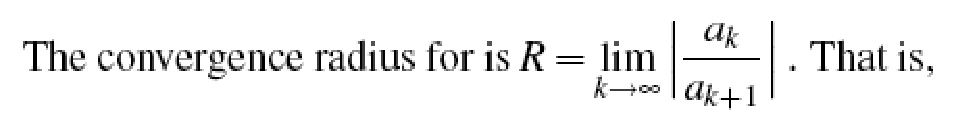
\includegraphics[width=0.55\textwidth]{latex}}}
	\subfigure[由Word软件生成的.doc格式行内公式]{\label{fig:subfig:word}
		\fbox{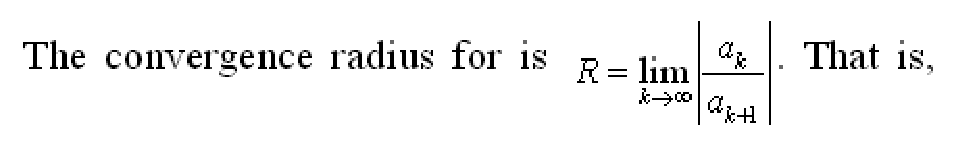
\includegraphics[width=0.55\textwidth]{word}}}
	\subfigure[由Word软件生成的.pdf格式行内公式]{\label{fig:subfig:pdf}
		\fbox{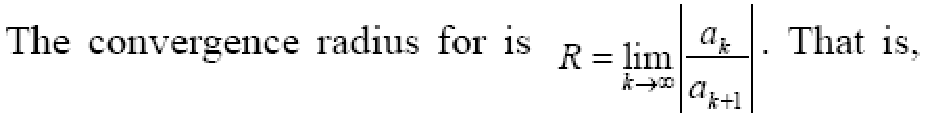
\includegraphics[width=0.55\textwidth]{pdf}}}

	\caption{由\LaTeX~和Word生成的3种行内公式屏显效果}\label{fig:hangju}
	\vspace{-1em}
\end{figure}

这三幅图分别为\LaTeX~和Word生成的行内公式屏显效果,从图中可看出,在\LaTeX~文本含有公式的行内,在正文与公式之间对接工整,行距不变;而在Word文本含有公式的行内,在正文与公式之间对接不齐,行距变大。因此从这一点来说,
\LaTeX~系统在数学公式的排版上具有很大优势。

\LaTeX~提供的行内公式最简单、最有效的方法是采用\TeX~本来的标记———开始和结束标记都写作\$,例如本段开始的例子可由下面的输入得到。
\verb|$f(x)=\int_{a}^{b}\frac{\sin{x}}{x}\mathrm{d}x$|

\section{行间公式}
位于两行之间的公式称为行间公式,每个公式都是一个单独的段落,例如
\[\int_a^b{f\left(x\right)\mathrm{d}x}=\lim_{\left\|\Delta{x_i}\right\|\to 0}\sum_i{f\left(\xi_i\right)\Delta{x_i}}\]
除人工编号外,\LaTeX~各种类型行间公式的标记见表\ref{tab:eqtag}。
\begin{table}[htbp]
	\caption{各种类型行间公式的标记}\label{tab:eqtag}
	\vspace{0.5em}\centering\zihao{5}
	\begin{tabularx}{\textwidth}{cll}
		\toprule
		         & 无编号                     & 自动编号                \\
		\midrule
		单行公式 & \verb|\begin{displaymath}... \end{displaymath}|    & \verb|\begin{equation}... \end{equation}| \\
		         & 或\verb|\[...\]| &                         \\
		多行公式 & \verb|\begin{eqnarray*}... \end{eqnarray*}|    & \verb|\begin{eqnarray}... \end{eqnarray}| \\
		\bottomrule
	\end{tabularx}
\end{table}

另外,在自动编号的某行公式行尾添加标签\verb|\nonumber|,可将该行转换为无编号形式。

行间多行公式需采用\verb|eqnarray|或\verb|eqnarray*|环境,它默认是一个列格式为\verb|rcl|的3列矩阵,并且中间列的字号要小一些,因此通常只将需要对齐的运算符号(通常为等号“=”)置于中间列。

\section{可自动调整大小的定界符}
若在左右两个定界符之前分别添加命令\verb|\left|和\verb|\right|,则定界符可根据所包围公式大小自动调整其尺寸,这可从式(\ref{nodelimiter})和式(\ref{delimiter})中看出。
\begin{equation}\label{nodelimiter}
	(\sum_{k=\frac12}^{N^2})
\end{equation}
\begin{equation}\label{delimiter}
	\left(\sum_{k=\frac12}^{N^2}\right)
\end{equation}
式(\ref{nodelimiter})和式(\ref{delimiter})是在\LaTeX~中分别输入如下代码得到的。
\begin{verbatim}
	(\sum_{k=\frac12}^{N^2})
	\left(\sum_{k=\frac12}^{N^2}\right)
\end{verbatim}
\verb|\left|和\verb|\right|总是成对出现的,若只需在公式一侧有可自动调整大小的定界符,则只要用“.”代替另一侧那个无需打印出来的定界符即可。

若想获得关于此部分内容的更多信息,可参见\href{http://tug.ctan.org/cgi-bin/ctanPackageInformation.py?id=voss-mathmode}{Math mode}文档的第8章“Brackets, braces and parentheses”。

\section{数学重音符号}
数学重音符号通常用来区分同一字母表示的不同变量,输入方法如下(需要调用\verb|amsmath|宏包):

\vspace{0.5em}\noindent\zihao{5}\begin{tabularx}{\textwidth}{Xc|Xc|Xc}
	\verb|\acute| & $\acute{a}$ & \verb|\mathring| & $\mathring{a}$           & \verb|\underbrace| & $\underbrace{a}$          \\
	\verb|\bar| & $\bar{a}$   & \verb|\overbrace| & $\overbrace{a}$          & \verb|\underleftarrow| & $\underleftarrow{a}$      \\
	\verb|\breve| & $\breve{a}$ & \verb|\overleftarrow| & $\overleftarrow{a}$      & \verb|\underleftrightarrow| & $\underleftrightarrow{a}$ \\
	\verb|\check| & $\check{a}$ & \verb|\overleftrightarrow| & $\overleftrightarrow{a}$ & \verb|\underline| & $\underline{a}$           \\
	\verb|\dddot| & $\dddot{a}$ & \verb|\overline| & $\overline{a}$           & \verb|\underrightarrow| & $\underrightarrow{a}$     \\
	\verb|\ddot| & $\ddot{a}$  & \verb|\overrightarrow| & $\overrightarrow{a}$     & \verb|\vec| & $\vec{a}$                 \\
	\verb|\dot| & $\dot{a}$   & \verb|\tilde| & $\tilde{a}$              & \verb|\widehat| & $\widehat{a}$             \\
	\verb|\grave| & $\grave{a}$ & \verb|\underbar| & $\underbar{a}$           & \verb|\widetilde| & $\widetilde{a}$           \\
	\verb|\hat| & $\hat{a}$
\end{tabularx}\vspace{0.5em}
\zihao{4} 当需要在字母$i$和$j$的上方添加重音符号时,为了去掉这两个字母顶上的小点,这两个字母应该分别改用\verb|\imath|和\verb|\jmath|。

如果遇到某些符号不知道该采用什么命令能输出它时,则可通过\href{http://detexify.kirelabs.org/classify.html}{Detexify$^2$网站}来获取符号命令。若用鼠标左键在此网页的方框区域内画出你所要找的符号形状,则会在网页右方列出和你所画符号形状相近的5个符号及其相对应的\LaTeX~输入命令。若所列出的符号中不包括你所要找的符号,还可通过点击“Select from the complete list!”以得分从低到高的顺序列出所有符号及其相对应的\LaTeX~输入命令。

最后,建议大家还以\href{http://tug.ctan.org/cgi-bin/ctanPackageInformation.py?id=voss-mathmode}{Math mode}这篇pdf文档作为主要参考。若要获得最为标准、美观的数学公式排版形式,可以查查文档中是否有和你所要的排版形式相同或相近的代码段,通过修改代码段以获得你所要的数学公式排版形式。


%%% !TEX encoding = UTF-8
\chapter{简要版帮助}
若您已很熟悉\LaTeX~的相关操作,建议阅读这份简要帮助说明。
\section{模板文件结构\label{sec:files}}
整个模板根目录的文件列表如下:
\begin{center}
	\begin{tabular}{|l|p{7.5cm}|l|}
		\hline
		HUNNUthesis.tex          &\TeX{}样例文件             & \textcolor{red}{{*}} \\
		\hline
		HUNNUthesis.cls&包含论文所使用的宏包和全文格式的定义。& \textcolor{red}{{*}} \\
		\hline
		HUNNUThesis.tex& 主文件,包含封面、扉页和其他章节的引用信息。& \textcolor{red}{{*}} \\
		\hline
		preface& 包含毕业设计论文的中英文摘要。& \textcolor{red}{{*}} \\
		\hline
		images& 包含封面用到的湖南师范大学Logo。& \textcolor{red}{{*}} \\
		\hline
		figures& 包含正文中所用到的图片。& \textcolor{red}{{*}} \\
		\hline
		body& 包含正文的所有章节。& \textcolor{red}{{*}} \\
		\hline
		appendix& 附件相关内容& \textcolor{red}{{*}} \\
		\hline
		appendix.tex & 作者的发表论文和参加科研情况说明& \textcolor{red}{{*}} \\
		\hline
		acknowledgements.tex&致谢文件& \textcolor{red}{{*}} \\
		\hline
		statement.tex&原创性说明和版权使用授权说明书。& \textcolor{red}{{*}} \\
		\hline
		hunnubib.bst             & 参考文献样式文件               & \textcolor{red}{{*}} \\
		\hline
		references/reference.bib & bib数据库                  & \textcolor{red}{{*}} \\
		\hline
		official\_documents& 学位论文的撰写格式和开题报告实施管理办法。& \\
		\hline
		clean.bat& 双击此文件,可以用来清理HUNNUThesis.tex在编译之后生成的所有附属文件,如后缀名为.aux,.log,.bak的文件。&  \\
		\hline
	\end{tabular}
\end{center}
注: \textcolor{red}{{*}} 表示\LaTeX{}模板必须的文件。
\subsection{文献引用}
将引文的bib数据库(默认文件名为reference.bib)放入模板根目录下的references文件夹,即可通过插入---文献引用自动产生引文。
\begin{itemize}
	\item 参考文献上标引用
	\begin{itemize}
		\item Journal:An article \upcite{ELIDRISSI94,MELLINGER96}。%参考文献上标
		\item An book \upcite{IEEE-1363,tex,companion}。%参考文献正常引用
		\item Conference:A conference \upcite{kocher99,DPMG,cnproceed}。
		\item Manual:A manual\upcite{NPB2}。
		\item MasterThesis:\upcite{zhubajie,metamori2004,shaheshang,FistSystem01}。
	\end{itemize}
	\item 参考文献正常引用
	\begin{itemize}
	\item Journal:An article \cite{ELIDRISSI94,MELLINGER96}。%参考文献上标
	\item An book \cite{IEEE-1363,tex,companion}。%参考文献正常引用
	\item Conference:A conference \cite{kocher99,DPMG,cnproceed}。
	\item Manual:A manual\cite{NPB2}。
	\item MasterThesis:\cite{zhubajie,metamori2004,shaheshang,FistSystem01}。
\end{itemize}
\end{itemize}
\subsection{伪代码实现}
\begin{algorithm}
	\caption{放进冰箱的大象}\label{算法实例}
	\begin{algorithmic}
		\REQUIRE 有一只大象
		\ENSURE 放进冰箱里
		\FOR {没有剩余的大象}
		\IF {大象比冰箱大}
		\STATE 把大象分割
		\ENDIF
		\ENDFOR
		\STATE 第一步
		\STATE 第二步
		\STATE 第三步
	\end{algorithmic}
	AAA\end{algorithm}
\subsection{代码展示}
可以把你的程序添加到附录里,展示自己的工作。
\begin{lstlisting}[language={[ANSI]C},
numbers=left,
numberstyle=\tiny,
basicstyle=\small\ttfamily,
stringstyle=\color{purple},
keywordstyle=\color{blue}\bfseries,
commentstyle=\color{olive},
directivestyle=\color{blue},
showstringspaces=false]
	#include <stdio.h>
	int main(int argc, char ** argv)
	{
		/*打印Hello,world*/
		printf("Hello, world!\n");
		
		return 0;
	}
\end{lstlisting}
\section{依赖}
HUNNUthesis依赖于以下宏包,这些宏包在常见的\LaTeX{}发行版中都包括,在安装使用之前,请确定你的\TeX{}发行版中都已正常安装这些宏包
\begin{table}[H]
	\centering
	\begin{tabular}{cccc}
\hline
{natbib} & {amsmath} & {amsfonts} & {amssymb} \\

{graphicx} & {subfigure} & {mathptmx} & {float} \\

{fontenc} & {booktabs} & {setspace} & {listings} \\

{xcolor} & {multirow} & {fancyhdr} & {etoolbox} \\

{tocloft} & {array} & {makecell} & {forloop} \\

{xstring} & {hyperref} & {cleveref} & {enumitem} \\

{algorithm} & {algorithmic} & {caption} & {ifthen} \\

{titlesec} & {ulem} & {amssymb} & {wasysym} \\

{flafter} & {booktabs} & {longtable} & {tabularx} \\

{setspace} & {subfigure} & {enumitem} & {calc } \\

{txfonts} & {bm} & {ntheorem} & {fancyvrb} \\

{xcolor} & {--} & {--} & {--} \\
\hline
	\end{tabular}
\end{table}
如果你尚未安装这些宏包,可以启动你的 \TeX{} 发行版的宏包管理器
来安装;或者到 \url{http://www.ctan.org} 上搜索下载并安装。
\section{基本设置}
\begin{enumerate}
	\item 论文正文所用图片搜索路径默认设置为模板根目录下的figures/。
	\item bib数据库默认设置为模板根目录下的references/reference.bib。 其中bib文件可由任意文献库管理软件自动生成
\end{enumerate}
\section{文字命令}
\subsection{常用命令}
\LaTeX 提供了一系列命令,用于修改字体、字号、数字等的呈现形式。
\subsubsection{字体}
ctex宏包及其文档类可直接使用以下六种字体:
\vspace{1em}\noindent\hrule
\begin{verbatim}
宋体: \songti       启用宋体  {\songti 宋体}。
黑体: \heiti        启用黑体  {\heiti 黑体}。
仿宋: \fangsong    启用仿宋   {\fangsong 仿宋}。
楷书: \kaishu       启用楷书   {\kaishu 楷书}。
隶书: \lishu        启用隶书  {\lishu 隶书}。
幼圆: \youyuan     启用幼圆   {\youyuan 幼圆}。
\end{verbatim}
\noindent\hrule\vspace{1em}

宋体:{\songti 宋体};黑体:{\heiti 黑体};仿宋:{\fangsong 仿宋};楷书:{\kaishu 楷书};隶书: {\lishu 隶书};幼圆: {\youyuan 幼圆}。
\subsubsection{字号}
{\bf 字号}%

\begin{center}
	\begin{tabular}{cccccccc}
		\toprule
		初号 & 小初 & 一号 & 小一 & 二号 & 小二 & 三号 & 小三 \\
		0    & -0   & 1    & -1   & 2    & -2   & 3    & -3   \\
		\hline
		四号 & 小四 & 五号 & 小五 & 六号 & 小六 & 七号 & 八号 \\
		4    & -4   & 5    & -5   & 6    & -6   & 7    & 8    \\
		\bottomrule
	\end{tabular}
\end{center}

\vspace{1em}\noindent\hrule
\begin{verbatim}
{\zihao{0}初号}; \dots {\zihao{4}四号};\dots 
\zihao{7}{七号} \zihao{4}
\end{verbatim}
\noindent\hrule\vspace{1em}

{\zihao{0}初号}; \dots {\zihao{4}四号};\dots \zihao{7}{七号}
\zihao{4}
%%% !TEX encoding = UTF-8
\addcontentsline{toc}{chapter}{结论}
\chapter*{结\quad 论}
结论单独作为一章排写,但不加章号。结论是毕业论文(设计)的总结,是整篇论文(设计)的归宿。要求精炼、准确地概述全文的主要观点:或自己赞成的观点、或自己反对的观点、或自己的创造性工作与新的见解及其意义和作用,还进一步提出需要讨论的问题和建议等。特别提醒这部分不是写你做毕业设计(论文)的感想,不是抒情。下面是一个分页符,可以另起一页

结论应是作者在学位论文研究过程中所取得的创新性成果的概要总结,不能与摘要混为一谈。
学位论文结论应包括论文的主要结果、创新点、展望三部分,在结论中应概括论文的核心观点,
明确、客观地指出本研究内容的创新性成果(含新见解、新观点、方法创新、技术创新、理论创新),并指出今后进一步在本研究方向进行研究工作的展望与设想。
对所取得的创新性成果应注意从定性和定量两方面给出科学、准确的评价,分(1)、(2)、(3)…条列出,宜用“提出了”、“建立了”等词叙述。

结论应是作者在学位论文研究过程中所取得的创新性成果的概要总结,不能与摘要混为一谈。
学位论文结论应包括论文的主要结果、创新点、展望三部分,在结论中应概括论文的核心观点,
明确、客观地指出本研究内容的创新性成果(含新见解、新观点、方法创新、技术创新、理论创新),并指出今后进一步在本研究方向进行研究工作的展望与设想。
对所取得的创新性成果应注意从定性和定量两方面给出科学、准确的评价,分(1)、(2)、(3)…条列出,宜用“提出了”、“建立了”等词叙述。

结论应是作者在学位论文研究过程中所取得的创新性成果的概要总结,不能与摘要混为一谈。
学位论文结论应包括论文的主要结果、创新点、展望三部分,在结论中应概括论文的核心观点,
明确、客观地指出本研究内容的创新性成果(含新见解、新观点、方法创新、技术创新、理论创新),并指出今后进一步在本研究方向进行研究工作的展望与设想。
对所取得的创新性成果应注意从定性和定量两方面给出科学、准确的评价,分(1)、(2)、(3)…条列出,宜用“提出了”、“建立了”等词叙述。

结论应是作者在学位论文研究过程中所取得的创新性成果的概要总结,不能与摘要混为一谈。
学位论文结论应包括论文的主要结果、创新点、展望三部分,在结论中应概括论文的核心观点,
明确、客观地指出本研究内容的创新性成果(含新见解、新观点、方法创新、技术创新、理论创新),并指出今后进一步在本研究方向进行研究工作的展望与设想。
对所取得的创新性成果应注意从定性和定量两方面给出科学、准确的评价,分(1)、(2)、(3)…条列出,宜用“提出了”、“建立了”等词叙述。
\end{verbatim}

\noindent\hrule\vspace{1em}

那么,编译的时候就只编译未加\%的一章,在这个例子中,即本章chapter1。

理论上,并不一定要把每章放在不同的文件中。但是这种自顶向下,分章节写作、编译的方法有利于提高效率,大大减少Debug过程中的编译时间,同时减小风险。
\section{参考文献生成方法}
\LaTeX~具有插入参考文献的能力。Google Scholar网站上存在兼容BibTeX的参考文献信息,通过以下几个步骤,可以轻松完成参考文献的生成。
\begin{itemize}
	\item 在\href{http://scholar.google.com/}{谷歌学术搜索}中,
	      点击\href{http://scholar.google.com/scholar_preferences?hl=en&as_sdt=0,5}{学术搜索设置}。
	\item 页面打开之后,在{\bf 文献管理软件}选项中选择{\bf 显示导入BibTeX的链接},单击保存设置,退出。
	\item 在谷歌学术搜索中检索到文献后,在文献条目区域单击导入BibTeX选项,页面中出现文献的引用信息。
	\item 将文献引用信息的内容复制之后,添加到references文件夹下的reference.bib中。
\end{itemize}
\section{编译注意事项}
\begin{enumerate}
	\item 由于模板使用UTF-8编码,所以源文件应该保存成UTF-8格式,否则可能出现中文字符无法识别的错误。
	      本模板中每一个.tex文件的文件的开头已经加上一行:\\
	      \verb|% !Mode:: "TeX:UTF-8"|\\
	      这样可以确保.tex文件默认使用UTF-8的格式打开。读者如果删去此行,很有可能会导致中文字符显示乱码。
	\item 建议采用以下编译方式:

	{\color{red}\heiti\bfseries XeLaTeX --> BibTeX --> XeLaTeX --> XeLaTeX}
\end{enumerate}
\section{系统要求}
TeX Live 2019或以上版本。使用推荐的TexStudio编辑器,可以完成文件的编辑和编译工作。
\section{\TeX~简介}
以下内容是milksea@bbs.ctex.org撰写的关于\TeX~的简单介绍,略有改动。
注意这不是一个入门教程,不讲\TeX~系统的配置安装,也不讲具体的\LaTeX~代码。
这里仅仅试图以一些只言片语来解释:
进入这个门槛之前新手应该知道的注意事项,以及遇到问题以后该去如何解决问题。
\subsection{什么是 \TeX/\LaTeX~,我是否应该选择它?}
\TeX~是最早由高德纳(Donald Knuth)教授创建的一门标记式宏语言,
用来排版科技文章,尤其擅长处理复杂的数学公式。\TeX~同时也是处理这一语言的排版软件。
\LaTeX~是 Leslie Lamport 在\TeX~基础上按内容/格式分离和模块化等思想建立的一集\TeX~上的格式。

\TeX~本身的领域是专业排版领域
但现在TeX/LaTeX也被广泛用于生成电子文档甚至幻灯片等,\TeX~语言的数学部分
偶尔也在其他一些地方使用。但注意\TeX~并不适用于文书处理(Microsoft Office 的领域,以前和现在都不是)。

选择使用\TeX/\LaTeX~的理由包括:
\begin{itemize}
	\item 免费软件;
	\item 专业的排版效果;
	\item 是事实上的专业数学排版标准;
	\item 广泛的西文期刊接收甚或只接收 LaTeX 格式的投稿;
	\item[] ……
\end{itemize}
不选择使用\TeX/\LaTeX~的理由包括:
\begin{itemize}
	\item 需要相当精力学习;
	\item 图文混合排版能力不够强;
	\item 仅在数学、物理、计算机等领域流行;
	\item 中文期刊的支持较差;
	\item[] ……
\end{itemize}

请尽量清醒看待网上经常见到的关于\TeX~与其他软件的优劣比较和口水战。在选择使用或离开之前,请先考虑
\TeX~的应用领域,想想它是否适合你的需要。
\subsection{我该用什么编辑器?}
编辑器功能有简有繁,特色不一,从简单的纯文本编辑器到繁复的 Emacs,因人而易。基本功能有语法高亮、方便编译预览就很好了,扩充功能和定制有无限的可能。初学者可以使用功能简单、使用方便的专用编辑器,如TexStudio、TeXWorks、Kile、WinEdt等,或者类似所见即所得功能的LyX;熟悉的人可以使用定制性更强的Notepad++、SciTE、Vim、Emacs 等。这方面的介绍很多,一开始不妨多试几种,找到最适合自己的才是最好的。

另外提醒一句,编辑器只是工作的助手,不必把它看得太重。
\subsection{我应该看什么\LaTeX~读物?}
这不是一个容易回答的问题,因为有许多选择,也同样有许多不合适的选择。
这里只是选出一个比较好的答案。更多更详细的介绍可以在版面和网上寻找(注意时效)。

近两年\TeX~的中文处理发展很快,目前没有哪本书在中文处理方面给出一个最新进展的合适综述,
因而下面的介绍也不主要考虑中文处理。

\begin{enumerate}
	\item 我能阅读英文。
	      \begin{enumerate}
		      \item 迅速入门:ltxprimer.pdf (LaTeX Tutorials: A Primer, India TUG)
		      \item 系统学习:A Guide to LaTeX, 4th Edition, Addison-Wesley
		            有机械工业出版社的影印版(《\LaTeX{}实用教程》)
		      \item 深入学习:要读许多书和文档,TeXbook 是必读的
		      \item 细节学习:去读你使用的每一个宏包的说明文档
		      \item 专题学习:阅读讲数学公式、图形、表格、字体等的专题文档
	      \end{enumerate}
	\item 我更愿意阅读中文。
	      \begin{enumerate}
		      \item 迅速入门:lnotes.pdf (LaTeX Notes, 1.20, Alpha Huang)
		      \item 系统学习:《\LaTeXe{}科技排版指南》,邓建松(电子版)
		            如果不好找,可以阅读《\LaTeXe~入门与提高》第二版,陈志杰等,或者 《\LaTeXe~完全学习手册》,胡伟
		      \item 深入学习:TeXbook0.pdf(特可爱原本,TeXbook 的中译,xianxian)
		      \item 具体问题释疑:CTeX-FAQ.pdf,\\
		            吴凌云,\url{http://www.ctex.org/CTeXFAQ}
	      \end{enumerate}
\end{enumerate}

遇见问题和解决问题的过程可以快速提高自己的技能,建议此时:
\begin{itemize}
	\item 利用Google搜索。
	\item 清楚,扼要地提出你的问题。
\end{itemize}

\subsection{什么知识会过时?什么不会?}
\TeX~是排版语言,也是广泛使用的软件,并且不断在发展中;
因此,总有一些东西会很快过时。作为学习\TeX~的人,
免不了要看各种各样的书籍、电子文档和网络论坛上的只言片语,
因此了解什么知识会迅速过时,什么知识不会是十分重要的。

最稳定的是关于Primitive \TeX~和Plain \TeX~的知识,也就是 Knuth
在他的《The TeXbook》中介绍的内容。因为\TeX~系统开发的初衷就是稳定性,要求今天的文档到很久以后仍可以得到完全相同的结果,
因此 Knuth 限定了他的\TeX~语言和相关实现的命令、语法。这些内容许多年来就没有多少变化,
在未来的一些年里也不会有什么变化。
Primitive \TeX~和 Plain \TeX~的知识主要包括 \TeX~排版的基本算法和原理,
盒子的原理,底层的 \TeX~命令等。其中技巧性的东西大多在宏包设计中,
初学者一般不会接触到很多;而基本原理则是常常被提到的,
譬如,\TeX~把一切排版内容作为盒子(box)处理。

相对稳定的是关于基本\LaTeXe~的知识,也包括围绕\LaTeXe~的一些核心宏包的知识。\LaTeXe~是自1993年以来的一个稳定的\LaTeX~版本,直到最近的一次修订(2005 年)都没有大的变动。\LaTeX~的下一个计划中的版本\LaTeX 3遥遥无期,在可预见的将来,\LaTeXe~不会过时。\LaTeXe~的知识是目前大部分\LaTeX~书籍的主体内容。关于\LaTeX~的标准文档类(article、report、book、letter、slide等),关于基本数学公式的输入,文档的章节层次,表格和矩阵,图表浮动体,LR 盒子与段落盒子……这些\LaTeX~的核心内容都是最常用的,相对稳定的。与\LaTeXe~相匹配的核心宏包,如graphics(x)、ifthen、fontenc、doc等,也同样是相对稳定的。还有一些被非常广泛应用的宏包,如amsmath系列,也可以看作是相对稳定的。

简单地说,关于基本\TeX/\LaTeX~的语言,都是比较稳定的。与之对应,实现或者支持\TeX/\LaTeX~语言的软件,包括在\TeX/\LaTeX~基础上建立的新的宏,都不大稳定。

容易过时的是关于第三方\LaTeX~宏包的知识、第三方\TeX~工具的知识,以及新兴\TeX~相关软件的知识等。\TeX~和\LaTeX~语言是追求稳定的;但无论是宏包还是工具,作为不断更新软件,它们是不稳定的。容易过时的技术很多,而且现在广泛地出现在几乎所有\LaTeX~文档之中,因此需要特别引起注意:宏包的过时的原因可能是宏包本身的升级换代带来了新功能或不兼容,也可能是同一功能的更新更好的宏包代替了旧的宏包。前者的典型例子比如绘图宏包PGF/TikZ,现在的2.00版功能十分强大,和旧的1.1x版相差很大,和更旧的0.x版本则几乎完全不同;后者的典型例子比如caption宏包先是被更新的caption2宏包代替,后来caption宏包更新又使得caption2 宏包完全过时。——安装更新的发行版可以避免使用过旧的宏包;认真阅读宏包自带的文档而不是搜索得到的陈旧片断可以避免采用过时的代码。

工具过时的主要原因也是升级换代和被其他工具替换。前者的典型例子是编辑器WinEdt在5.5以后的版本支持UTF-8编码,而旧版本不支持;后者的典型例子是中文字体安装工具从GBKFonts到xGBKFonts到FontsGen不断被取代。图形插入是一个在\TeX~实现、宏包与外围工具方面都更新很快的东西。在过去,最常用的输出格式是PS(PostScript)格式,因此插入的图像以EPS为主流。使用Dvips为主要输出工具,外围工具有GhostScript、bmeps等等,相关宏包有graphics等,相关文档如《\LaTeXe{} 插图指南》。

但凡提及“\LaTeX~只支持EPS图形”的,就是这个过时的时代的产物。事实上\TeX/\LaTeX~并不限定任何图形格式,只不过是当时的输出格式(PS)和工具(Dvips)对EPS情有独钟而已。后来 PDF 格式成为主流。pdf\TeX~、DVIPDFM、DVIPDFMx、XeTeX工具则主要支持PDF、PNG、JPG格式的图形,涉及一系列工具如ImageMagick、ebb等。

值得特别提出注意的就是,中文处理也一起是更新迅速、容易过时的部分。而且因为中文处理一直没有一个“官方”的“标准”做法,软件、工具、文档以及网上纷繁的笔记也就显得相当混乱。从八十年代开始的CCT系统、天元系统,到后来的CJK方式,到近来的XeTeX和LuaTeX 方式,中文处理的原理、软件、宏包、配置方式等都在不断变化中。
\section{免责声明}
本模板依据《湖南师范大学研究生学位论文的撰写格式》编写,适用于所有博士、硕士生的学位论文编写。然而,作者不保证本模板完全符合学校要求,也不对由此带来的风险和损失承担任何责任。